%definira klasu dokumenta 
\documentclass[12pt]{report} 

%prostor izmedu naredbi \documentclass i \begin{document} se zove uvod. U njemu se nalaze naredbe koje se odnose na cijeli dokument

%osnovni LaTex ne može riješiti sve probleme, pa se koriste različiti paketi koji olakšavaju izradu željenog dokumenta
\usepackage[croatian]{babel} 
\usepackage{amssymb}
\usepackage{amsmath}
\usepackage{txfonts}
\usepackage{mathdots}
\usepackage{titlesec}
\usepackage{array}
\usepackage{lastpage}
\usepackage{etoolbox}
\usepackage{tabularray}
\usepackage{color, colortbl}
\usepackage{adjustbox}
\usepackage{geometry}
\usepackage[classicReIm]{kpfonts}
\usepackage{hyperref}
\usepackage{fancyhdr}
\usepackage[justification=centering]{caption}

\usepackage{float}
\usepackage{setspace}
\restylefloat{table}

\usepackage{indentfirst}
\usepackage[T1]{fontenc}
\usepackage{graphicx}


\patchcmd{\chapter}{\thispagestyle{plain}}{\thispagestyle{fancy}}{}{} %redefiniranje stila stranice u paketu fancyhdr

%oblik naslova poglavlja
\titleformat{\chapter}{\normalfont\huge\bfseries}{\thechapter.}{20pt}{\Huge}
\titlespacing{\chapter}{0pt}{0pt}{40pt}


\linespread{1.3} %razmak između redaka

\geometry{a4paper, left=1in, top=1in,}  %oblik stranice

\hypersetup{ colorlinks, citecolor=black, filecolor=black, linkcolor=black,	urlcolor=black }   %izgled poveznice


%prored smanjen između redaka u nabrajanjima i popisima
\newenvironment{packed_enum}{
	\begin{enumerate}
		\setlength{\itemsep}{0pt}
		\setlength{\parskip}{0pt}
		\setlength{\parsep}{0pt}
	}{\end{enumerate}}

\newenvironment{packed_item}{
	\begin{itemize}
		\setlength{\itemsep}{0pt}
		\setlength{\parskip}{0pt}
		\setlength{\parsep}{0pt}
	}{\end{itemize}}




%boja za privatni i udaljeni kljuc u tablicama
\definecolor{LightBlue}{rgb}{0.9,0.9,1}
\definecolor{LightGreen}{rgb}{0.9,1,0.9}

%Promjena teksta za dugačke tablice
\DefTblrTemplate{contfoot-text}{normal}{Nastavljeno na idućoj stranici}
\SetTblrTemplate{contfoot-text}{normal}
\DefTblrTemplate{conthead-text}{normal}{(Nastavljeno)}
\SetTblrTemplate{conthead-text}{normal}
\DefTblrTemplate{middlehead,lasthead}{normal}{Nastavljeno od prethodne stranice}
\SetTblrTemplate{middlehead,lasthead}{normal}

%podesavanje zaglavlja i podnožja

\pagestyle{fancy}
\lhead{Programsko inženjerstvo}
\rhead{Eventko}
\lfoot{Vidoje}
\cfoot{stranica \thepage/\pageref{LastPage}}
\rfoot{\today}
\renewcommand{\headrulewidth}{0.2pt}
\renewcommand{\footrulewidth}{0.2pt}


\begin{document} 
	
	
	
	\begin{titlepage}
		\begin{center}
			\vspace*{\stretch{1.0}} %u kombinaciji s ostalim \vspace naredbama definira razmak između redaka teksta
			\LARGE Programsko inženjerstvo\\
			\large Ak. god. 2022./2023.\\
			
			\vspace*{\stretch{3.0}}
			
			\huge Interaktivni socijalni kalendar Eventko\\
			\Large Dokumentacija, Rev. 1\\
			
			\vspace*{\stretch{12.0}}
			\normalsize
			Grupa: \textit{Vidoje}\\
			Voditelj: \textit{Velimir Kovačić}\\
			
			
			\vspace*{\stretch{1.0}}
			Datum predaje: \textit{18. 11. 2022.}\\
	
			\vspace*{\stretch{4.0}}
			
			Nastavnik: \textit{Miljenko Krhen}\\
		
		\end{center}

	
	\end{titlepage}

	
	\tableofcontents


	\chapter{Dnevnik promjena dokumentacije}
				
		\begin{longtblr}[
				label=none
			]{
				width = \textwidth, 
				colspec={|X[2]|X[13]|X[3]|X[3]|}, 
				rowhead = 1
			}
			\hline
			\textbf{Rev.}	& \textbf{Opis promjene/dodatka} & \textbf{Autori} & \textbf{Datum}\\[3pt] \hline
			0.1 & Napravljen predložak.	& * & 03.11.2022. 		\\[3pt] \hline 
			0.2	& Dodan detaljan opis projekta. Popunjen dosadašnji dnevnik sastajanja. Dodani obrasci uporabe i funkcionalni zahtjevi. & *'** & 14.11.2022. 	\\[3pt] \hline 
			0.5 & Dodan \textit{Use Case} dijagram i jedan sekvencijski dijagram, funkcionalni i nefunkcionalni zahtjevi i dodatak A & * & 25.08.2013. \\[3pt] \hline 
			0.6 & Arhitektura i dizajn sustava, algoritmi i strukture podataka & * & 26.08.2013. \\[3pt] \hline 
			0.8 & Povijest rada i trenutni status implementacije,\newline Zaključci i plan daljnjeg rada & * & 28.08.2013. \\[3pt] \hline 
			0.9 & Opisi obrazaca uporabe & * & 07.09.2013. \\[3pt] \hline 
			0.10 & Preveden uvod & * & 08.09.2013. \\[3pt] \hline 
			0.11 & Sekvencijski dijagrami & * & 09.09.2013. \\[3pt] \hline 
			0.12.1 & Započeo dijagrame razreda & * & 10.09.2013. \\[3pt] \hline 
			0.12.2 & Nastavak dijagrama razreda & * & 11.09.2013. \\[3pt] \hline 
			\textbf{1.0} & Verzija samo s bitnim dijelovima za 1. ciklus & * & 11.09.2013. \\[3pt] \hline 
			1.1 & Uređivanje teksta -- funkcionalni i nefunkcionalni zahtjevi & * \newline * & 14.09.2013. \\[3pt] \hline 
			1.2 & Manje izmjene:Timer - Brojilo vremena & * & 15.09.2013. \\[3pt] \hline 
			1.3 & Popravljeni dijagrami obrazaca uporabe & * & 15.09.2013. \\[3pt] \hline 
			1.5 & Generalna revizija strukture dokumenta & * & 19.09.2013. \\[3pt] \hline 
			1.5.1 & Manja revizija (dijagram razmještaja) & * & 20.09.2013. \\[3pt] \hline 
			\textbf{2.0} & Konačni tekst predloška dokumentacije  & * & 28.09.2013. \\[3pt] \hline 
			&  &  & \\[3pt] \hline	
		\end{longtblr}
	
	
		\textit{Moraju postojati glavne revizije dokumenata 1.0 i 2.0 na kraju prvog i drugog ciklusa. Između tih revizija mogu postojati manje revizije već prema tome kako se dokument bude nadopunjavao. Očekuje se da nakon svake značajnije promjene (dodatka, izmjene, uklanjanja dijelova teksta i popratnih grafičkih sadržaja) dokumenta se to zabilježi kao revizija. Npr., revizije unutar prvog ciklusa će imati oznake 0.1, 0.2, …, 0.9, 0.10, 0.11.. sve do konačne revizije prvog ciklusa 1.0. U drugom ciklusu se nastavlja s revizijama 1.1, 1.2, itd.}
	\chapter{Opis projektnog zadatka}
		
		\indent Cilj ovog projekta je razviti programsku podršku za stvaranje web aplikacije "Eventko". Ova aplikacija omogućit će korisnicima da kvalitetnije i jednostavnije stvaraju i upisuju se na događaje. Aplikacija će pružati uvid u sve trenutne javne događaje kojima se može pristupiti. Događaji će biti prikazani u obliku kalendara koji je inspiriran izgledom kalendara u aplikaciji Ferko. \\
			
		\indent Prilikom prvog pokretanja aplikacije korisnik se nalazi na stranici za prijavu na kojoj će se prikazati prozorčić s poljima za potrebne podatke:
		
		\begin{packed_item}
			\item polje za unos korisničkog imena profila
			\item polje za unos lozinke korisničkog profila
			\item gumb za prijavu
			\item gumb za izradu novog računa (\textit{sign up})
		\end{packed_item}
		
		\indent Tijekom prvog pokretanja profil još nije napravljen tako da je potrebno stisnuti gumb \textit{Izradi račun} kako bi se napravio novi korisnički profil. Nakon pritiska gumba aplikacija prebacuje korisnika na novu stranicu na kojoj je prikazan prozor s poljima za unos potrebnih podataka za izradu novog profila, kao i gumbi za registraciju ili za povratak na stranicu za prijavu. Za registraciju novog profila potrebni su sljedeći podaci:
		
		\begin{packed_item}
			\item korisničko ime
			\item nadimak (neobavezno)
			\item lozinka
			\item ponovljena lozinka
			\item e-mail adresa
		\end{packed_item}
	
		\indent Nakon što su podaci uspješno uneseni potrebno je stisnuti gumb "Izradi" kako bi se novi korisnički profil generirao. Po uspješnom stvaranju korisnik je prebačen natrag na stranicu za prijavu te se može prijaviti svojim novim korisničkim računom. Nakon uspješne prijave aplikacija vodi korisnika na početnu stranicu.
		\eject
		
		\indent Na početnoj stranici prikazana je alatna traka na kojoj su redom nanizani sljedeći objekti:
		
		\begin{packed_item}
			\item logotip aplikacije Eventko
			\item Obavijesti
			\item Moji prijatelji
			\item Pohađani događaji
			\item Moj profil
			\item Odjava
		\end{packed_item}
	
		\indent Ispod alatne trake prikazan je gumb \textit{Stvori novi događaj} kojim je moguće kreiranje novog javnog ili privatnog događaja te osobne obaveze. Odabir otvara novi prozorčić u koji je potrebno napisati sljedeće podatke:
		
		\begin{packed_item}
			\item Vrsta događaja
			\item Naslov
			\item Lokacija (omogućen prikaz na Google Kartama uz API)
			\item Datum i vrijeme
			\item Oznake događaja (npr. kava, učenje, društvene igre...)
			\item Opis događaja
		\end{packed_item}
	
		\indent Ispod gumba \textit{Stvori novi događaj} nalaze se liste aktivnih korisnika te istaknutih događaja koje uređuju moderatori. Većinu prikaza stranice zauzima središnji kalendar na kojem su vidljive sve korisnikove obaveze te događaji kojima je odabrao prisustvovati ili koje sam organizira. Prikazuje se tekući tjedan, a moguće je listati i one nadolazeće. \\
		
		\indent S desne strane nalazi se sekcija \textit{Javni događaji} s gumbom \textit{Izbornik} koji otvara padajući izbornik s nadolazećim javnim događajima u kojima je moguće sudjelovati. Odabir pojedinog događaja privremeno ga prikazuje u kalendaru te su klikom na njega vidljive osnovne informacije i oznake, kao i opcija prijave čime je dodan u korisnikov kalendar. \\
		
		\indent Odabir kartice \textit{Obavijesti} prikazuje listu obavijesti inicijalno poredanih od najnovijih prema starijim. Korisnik može biti obaviješten da je privremeno ili trajno suspendiran, promaknut u moderatora i slično.
		\eject
		
		\indent Odabir kartice \textit{Moji prijatelji} otvara stranicu koja prikazuje listu trenutnih prijatelja korisnika, a s desne strane nalazi se gumb za pretraživanje korisnika po korisničkom imenu te gumb za dodavanje prijatelja pomoću QR koda. \\
		
		\indent Odabir kartice \textit{Pohađani događaji} prebacuje korisnika na novu stranicu sa svim događajima na kojima je korisnik sudjelovao i bit će mu omogućeno da ih označi sa \textit{Sviđa mi se} ili \textit{Ne sviđa mi se}. \\
		
		\indent Odabir kartice \textit{Moj profil} otvara stranicu koja prikazuje korisnikove podatke:
		
		\begin{packed_item}
			\item nadimak, uz opciju izmjene
			\item korisničko ime
			\item e-mail adresa
			\item jedinstveni korisnički QR kod
			\item ukoliko je riječ o običnom korisniku, opcija pretplate za Premium račun
		\end{packed_item}
		
		\indent Odabir kartice \textit{Odjava} vraća korisnika na stranicu za prijavu. \\
		
		\indent Različite uloge u aplikaciji su sljedeće:
		
		\begin{packed_item}
			\item Običan korisnik
			\item Premium korisnik
			\item Pregledavač
			\item Moderator
			\item Administrator
		\end{packed_item}
	
		\indent Pregledavač je korisnik na uvodnoj stranici za prijavu koji trenutno nije prijavljen. Običnom korisniku dostupne su sve funkcionalnosti prethodno opisane. \\
		
		\indent Premium korisnik ima sve mogućnosti običnoga uz dodatnu opciju promoviranja određenog broja događaja koje organizira, čime se oni prikazuju na listi istaknutih događaja na lijevoj strani stranice. \\
		
		\indent Moderator ima sve mogućnosti premium korisnika, uz to što ima dodatnu karticu na alatnoj traci imena \textit{Upravljanje korisnicima}, koja ga prebacuje na novu stranicu na kojoj može suspendirati korisnike koji se ne ponašaju u skladu s bontonom aplikacije. Također ima opciju \textit{Izmjeni oznake} na događajima kako bi mogao dodati ili ukloniti oznake po potrebi. Konačno, ima opciju \textit{Izbriši event} ako je neki javni događaj neprimjeren. \\
		
		\indent Administrator ima sve mogućnosti moderatora uz to što može na stranici za upravljanje korisnicima ili promovirati posebno vrijedne članove zajednice u moderatore, ili obrisati račune korisnika koji uporno krše pravila i nakon privremene suspenzije.
		
		\section{Primjeri u \LaTeX u}
		
		\textit{Ovo potpoglavlje izbrisati.}\\

		U nastavku se nalaze različiti primjeri kako koristiti osnovne funkcionalnosti \LaTeX a koje su potrebne za izradu dokumentacije. Za dodatnu pomoć obratiti se asistentu na projektu ili potražiti upute na sljedećim web sjedištima:
		\begin{itemize}
			\item Upute za izradu diplomskog rada u \LaTeX u - \url{https://www.fer.unizg.hr/_download/repository/LaTeX-upute.pdf}
			\item \LaTeX\ projekt - \url{https://www.latex-project.org/help/}
			\item StackExchange za Tex - \url{https://tex.stackexchange.com/}\\
		
		\end{itemize} 	


		
		\noindent \underbar{podcrtani tekst}, \textbf{podebljani tekst}, 	\textit{nagnuti tekst}\\
		\noindent \normalsize primjer \large primjer \Large primjer \LARGE {primjer} \huge {primjer} \Huge primjer \normalsize
				
		\begin{packed_item}
			
			\item  primjer
			\item  primjer
			\item  primjer
			\item[] \begin{packed_enum}
				\item primjer
				\item[] \begin{packed_enum}
					\item[] primjer
					\item[b] primjer
				\end{packed_enum}
				\item primjer
			\end{packed_enum}
			
		\end{packed_item}
		
		\indent primjer url-a: \url{https://www.fer.unizg.hr/predmet/proinz/projekt}
		
		\noindent posebni znakovi: \# \$ \% \& \{ \} \_ 
		$|$ $<$ $>$ 
		\^{} 
		\~{} 
		$\backslash$ 
		
		
		\begin{longtblr}[
			label=none,
			entry=none
			]{
				width = \textwidth,
				colspec={|X[8,l]|X[8, l]|X[16, l]|}, 
				rowhead = 1,
			} %definicija širine tablice, širine stupaca, poravnanje i broja redaka naslova tablice
			\hline \multicolumn{3}{|c|}{\textbf{naslov unutar tablice}}	 \\ \hline[3pt]
			\SetCell{LightGreen}IDKorisnik & INT	&  	Lorem ipsum dolor sit amet, consectetur adipiscing elit, sed do eiusmod  	\\ \hline
			korisnickoIme	& VARCHAR &   	\\ \hline 
			email & VARCHAR &   \\ \hline 
			ime & VARCHAR	&  		\\ \hline 
			\SetCell{LightBlue} primjer	& VARCHAR &   	\\ \hline 
		\end{longtblr}
		

		\begin{longtblr}[
				caption = {Naslov s referencom izvan tablice},
				entry = {Short Caption},
			]{
				width = \textwidth, 
				colspec = {|X[8,l]|X[8,l]|X[16,l]|}, 
				rowhead = 1,
			}
			\hline
			\SetCell{LightGreen}IDKorisnik & INT	&  	Lorem ipsum dolor sit amet, consectetur adipiscing elit, sed do eiusmod  	\\ \hline
			korisnickoIme	& VARCHAR &   	\\ \hline 
			email & VARCHAR &   \\ \hline 
			ime & VARCHAR	&  		\\ \hline 
			\SetCell{LightBlue} primjer	& VARCHAR &   	\\ \hline 
		\end{longtblr}
	


		
		
		%unos slike
		\begin{figure}[H]
			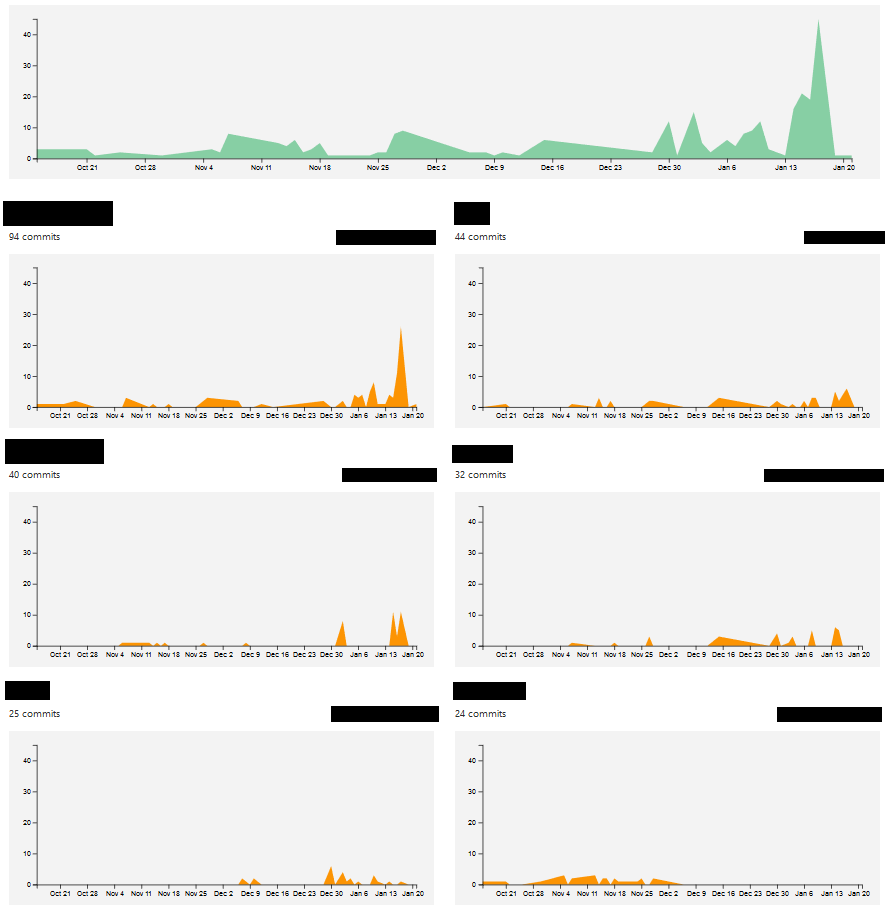
\includegraphics[scale=0.4]{slike/aktivnost.PNG} %veličina slike u odnosu na originalnu datoteku i pozicija slike
			\centering
			\caption{Primjer slike s potpisom}
			\label{fig:promjene}
		\end{figure}
		
		\begin{figure}[H]
			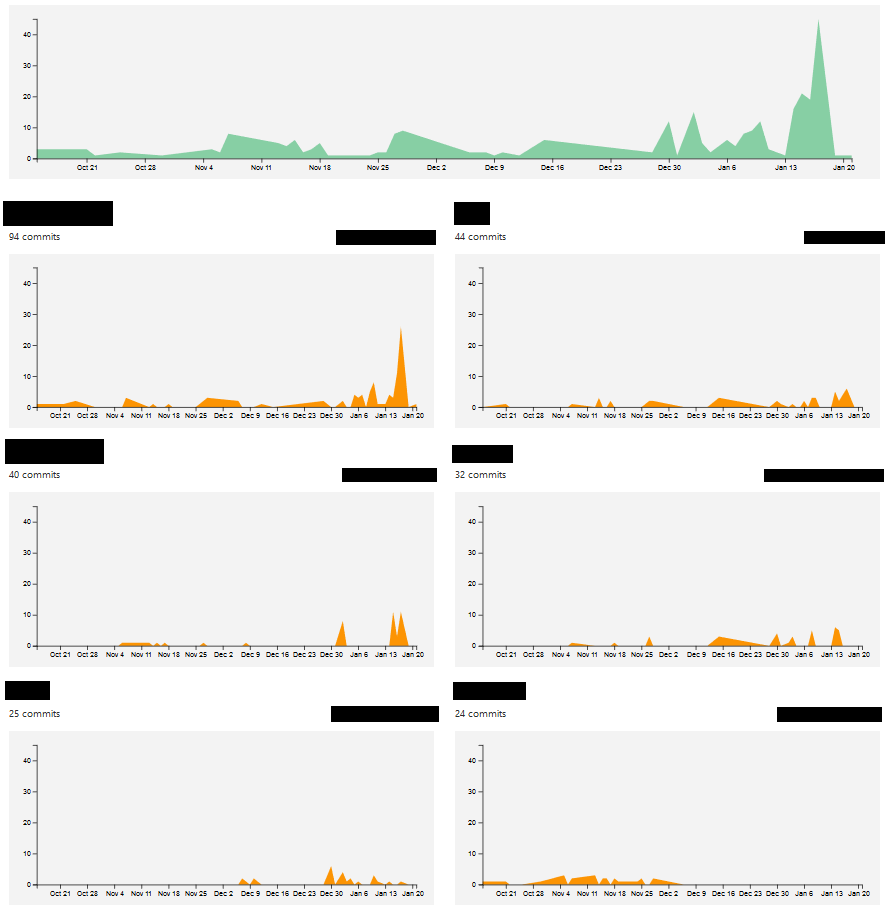
\includegraphics[width=\textwidth]{slike/aktivnost.PNG} %veličina u odnosu na širinu linije
			\caption{Primjer slike s potpisom 2}
			\label{fig:promjene2} %label mora biti drugaciji za svaku sliku
		\end{figure}
		
		Referenciranje slike \ref{fig:promjene2} u tekstu.
		
		\eject
		
	
	\chapter{Specifikacija programske potpore}
		
	\section{Funkcionalni zahtjevi}
			

			

				

			
			
			\noindent \textbf{Dionici:}
			
			\begin{packed_enum}
				
				\item Administrator
				\item Moderator			
				\item Korisnici aplikacije
					\begin{packed_enum}
						
						\item  Pregledavač
						\item  Običan korisnik
						\item  Premium korisnik
					
					\end{packed_enum}
				\item Razvojni tim	
				
			\end{packed_enum}
			
			\noindent \textbf{Aktori i njihovi funkcionalni zahtjevi:}
			
			
			\begin{packed_enum}
				\item  \underbar{Pregledavač/neprijavljen korisnik (inicijator) može:}
				
				\begin{packed_enum}
					
					\item 	Otvoriti stranicu za prijavu
					\item   Izvršiti prijavu
					\item 	Otvoriti stranicu za registraciju
					\item   Izvršiti registraciju
					
					
				\end{packed_enum}
			
				\item  \underbar{Običan korisnik (inicijator) može:}
				
				\begin{packed_enum}
					
					\item Dodati obveze, javne i privatne događaje
					\item Ocjenjivati posjećene događaje
					\item Prijavljivati se na događaje
					\item Preko nadimka ili QR koda dodati prijatelje
					\item Ukloniti prijatelje
					\item Blokirati korisnike
					\item Promijeniti nadimak profila
					\item Pretplatiti se na premium račun
					
				\end{packed_enum}
			
				\item  \underbar{Premium korisnik (inicijator) može:}
				
				\begin{packed_enum}
					
					\item Promovirati vlastiti događaj
			
					
				\end{packed_enum}
			
				\item  \underbar{Moderator (inicijator) može:}
				
				\begin{packed_enum}
					
					\item Suspendirati korisnika
					\item Uređivati oznake javnih događaja
					\item Brisati događaje
					
				\end{packed_enum}
			
				\item  \underbar{Administrator (inicijator) može:}
				
				\begin{packed_enum}
					
					\item Promovirati korisnika u moderatora
					\item Brisati korisničke račune
					
				\end{packed_enum}
			
				\item  \underbar{Baza podataka (sudionik):}
				
				\begin{packed_enum}
					
					\item Pohranjuje sve podatke o korisnicima i njihovim ovlastima
					\item Pohranjuje sve podatke o događajima i njihovim karakteristikama
					
				\end{packed_enum}
			
			
			\end{packed_enum}
			
			\eject 
			
			
				
			\subsection{Obrasci uporabe}
				
				
				
				\subsubsection{Opis obrazaca uporabe}
					
					

					\noindent \underbar{\textbf{UC1 - Registracija}}
					\begin{packed_item}
						
						\item \textbf{Glavni sudionik: }Pregledavač
						\item  \textbf{Cilj:} registracija
						\item  \textbf{Sudionici:}
						Baza podataka
						\item  \textbf{Preduvjet:} korisnik nije prijavljen u aplikaciji
						\item  \textbf{Opis osnovnog tijeka:}
						
						\item[] \begin{packed_enum}
							
							\item	Otvaranjem aplikacije otvara se stranica za prijavu
							\item	Pritisne se gumb \textit{Izradi račun}
							\item	Unesu se potrebni podaci i pritisne gumb \textit{Izradi}
							
						\end{packed_enum}
						
						\item  \textbf{Opis mogućih odstupanja:}
						
						\item[] \begin{packed_item}
							
							\item[3.a] Korisnik ne unese pravilno potrebne podatke
							
						\end{packed_item}
					\end{packed_item}
					
					\noindent \underbar{\textbf{UC2 - Prijava}}
					\begin{packed_item}
						
						\item \textbf{Glavni sudionik: }Pregledavač
						\item  \textbf{Cilj:} prijava
						\item  \textbf{Sudionici:}
						Baza podataka
						\item  \textbf{Preduvjet:} korisnik nije prijavljen u aplikaciji, ali je registriran
						\item  \textbf{Opis osnovnog tijeka:}
						
						\item[] \begin{packed_enum}
							
							\item	Otvaranjem aplikacije otvara se stranica za prijavu
							\item	Upišu se potrebni podaci
							\item	Pritisne se gumb \textit{Prijava}
							
						\end{packed_enum}
						
						\item  \textbf{Opis mogućih odstupanja:}
						
						\item[] \begin{packed_item}
							
							\item[2.a] Korisnik ne unese pravilno potrebne podatke 
							
						\end{packed_item}
					\end{packed_item}
					
					\noindent \underbar{\textbf{UC3 - Promocija vlastitih događaja}}
					\begin{packed_item}
						
						\item \textbf{Glavni sudionik: }Premium korisnik
						\item  \textbf{Cilj:} isticanje svojih događaja drugim korisnicima
						\item  \textbf{Sudionici:}
						Baza podataka
						\item  \textbf{Preduvjet:} korisnik prijavljen i kupljen je premium profil
						\item  \textbf{Opis osnovnog tijeka:}
						
						\item[] \begin{packed_enum}
							
							\item	Na Početnoj stranici pritisne se gumb \textit{Dodaj u kalendar}
							\item	Stvori se novi događaj i klikne se gumb \textit{Promoviraj događaj}
							
						\end{packed_enum}
					\end{packed_item}
					
					\noindent \underbar{\textbf{UC4 - Blokiranje korisnika}}
					\begin{packed_item}
						
						\item \textbf{Glavni sudionik: }Korisnik
						\item  \textbf{Cilj:} blokiranje korisničkog računa
						\item  \textbf{Sudionici:}
						Baza podataka
						\item  \textbf{Preduvjet:} korisnik prijavljen
						\item  \textbf{Opis osnovnog tijeka:}
						
						\item[] \begin{packed_enum}
							
							\item	Pritiskom na karticu \textit{Moji prijatelji} na alatnoj traci otvara se stranica za dodavanje prijatelja
							\item	Na sekciji \textit{Pretraži korisnike} unosi se željeno korisničko ime
							\item	Pritiskom na opciju \textit{Blokiraj korisnika} željeni korisnik je blokiran.
							
						\end{packed_enum}
						
						\item  \textbf{Opis mogućih odstupanja:}
						
						\item[] \begin{packed_item}
							
							\item[2.a] Uneseno nepostojeće korisničko ime
							
						\end{packed_item}
					\end{packed_item}
					
					\noindent \underbar{\textbf{UC5 - Pretplata za premium}}
					\begin{packed_item}
						
						\item \textbf{Glavni sudionik: }Korisnik
						\item  \textbf{Cilj:} Pretplata na premium profil
						\item  \textbf{Sudionici:}
						Baza podataka
						\item  \textbf{Preduvjet:} korisnik prijavljen kao običan korisnik
						\item  \textbf{Opis osnovnog tijeka:}
						
						\item[] \begin{packed_enum}
							
							\item	Pritiskom na karticu \textit{Korisnik} na alatnoj traci otvara se profil korisnika
							\item Pritiskom na gumb \textit{Pretplati se na Premium} dobiva se premium profil
							
						\end{packed_enum}
					\end{packed_item}
					
					\noindent \underbar{\textbf{UC6 - Izmjena nadimka}}
					\begin{packed_item}
						
						\item \textbf{Glavni sudionik: }Korisnik
						\item  \textbf{Cilj:} izmijeniti korisnički nadimak
						\item  \textbf{Sudionici:}
						Baza podataka
						\item  \textbf{Preduvjet:} korisnik prijavljen
						\item  \textbf{Opis osnovnog tijeka:}
						
						\item[] \begin{packed_enum}
							
							\item	Klikom na vlastito korisničko ime na alatnoj traci korisnik je prebačen na stranicu svog profila
							\item	Odabire \textit{Promjeni nadimak} i upisuje novi željeni nadimak koji ne mora biti jedinstven
							
						\end{packed_enum}
					\end{packed_item}
					
					\noindent \underbar{\textbf{UC7 - Dodavanje prijatelja korisničkim imenom}}
					\begin{packed_item}
						
						\item \textbf{Glavni sudionik: }Korisnik
						\item  \textbf{Cilj:} dodavanje prijatelja
						\item  \textbf{Sudionici:}
						Baza podataka
						\item  \textbf{Preduvjet:} korisnik prijavljen
						\item  \textbf{Opis osnovnog tijeka:}
						
						\item[] \begin{packed_enum}
							
							\item	Pritiskom na karticu \textit{Moji prijatelji} na alatnoj traci otvara se stranica za dodavanje prijatelja
							\item	Prijatelja se može dodati upisivanjem korisničkog imena korisnika
							
						\end{packed_enum}
						
						\item  \textbf{Opis mogućih odstupanja:}
						
						\item[] \begin{packed_item}
							
							\item[2.a] Unesen nepostojeći korisnik
							
						\end{packed_item}
					\end{packed_item}
					
					\noindent \underbar{\textbf{UC8 - Dodavanje prijatelja QR kodom}}
					\begin{packed_item}
						
						\item \textbf{Glavni sudionik: }Korisnik
						\item  \textbf{Cilj:} lakši i brži način dodavanja prijatelja QR kodom
						\item  \textbf{Sudionici:}
						Baza podataka
						\item  \textbf{Preduvjet:} korisnik prijavljen
						\item  \textbf{Opis osnovnog tijeka:}
						
						\item[] \begin{packed_enum}
							
							\item	Pritiskom na karticu \textit{Moji prijatelji} na alatnoj traci na početnoj stranici otvara se stranica
							\item	Prikazan je vlastiti QR kod preko API-a
							\item	Prijatelj preko svog mobitela skenira QR kod i dodaje prijatelja
							
						\end{packed_enum}
						
					\end{packed_item}
					
					\noindent \underbar{\textbf{UC9 - Uklanjanje prijatelja}}
					\begin{packed_item}
						
						\item \textbf{Glavni sudionik: }Korisnik
						\item  \textbf{Cilj:} uklanjanje prijatelja
						\item  \textbf{Sudionici:}
						Baza podataka
						\item  \textbf{Preduvjet:} korisnik prijavljen
						\item  \textbf{Opis osnovnog tijeka:}
						
						\item[] \begin{packed_enum}
							
							\item	Pritiskom na karticu \textit{Moji prijatelji} na alatnoj traci otvara se stranica za dodavanje prijatelja
							\item	Prijatelja se može ukloniti s liste izborom \textit{Ukloni prijatelja}
							
						\end{packed_enum}
					\end{packed_item}
					
					\noindent \underbar{\textbf{UC10 - Stvaranje događaja}}
					\begin{packed_item}
						
						\item \textbf{Glavni sudionik: }Korisnik
						\item  \textbf{Cilj:} stvaranje događaja u kalendaru
						\item  \textbf{Sudionici:}
						Baza podataka
						\item  \textbf{Preduvjet:} korisnik prijavljen
						\item  \textbf{Opis osnovnog tijeka:}
						
						\item[] \begin{packed_enum}
							
							\item	Sa lijeve strane Početne stranice prikazan je gumb \textit{Dodaj u kalendar}
							\item 	Otvara se prozor u koji se unose potrebni podaci i oznake
							\item[] \begin{packed_enum}
								\item Ukoliko je odabran privatan događaj poziva se željene prijatelje
							\end{packed_enum}
							
						\end{packed_enum}
						
						\item  \textbf{Opis mogućih odstupanja:}
						
						\item[] \begin{packed_item}
							
							\item[2.a] Pogrešno uneseni podaci
							
						\end{packed_item}
					\end{packed_item}
					
					\noindent \underbar{\textbf{UC11 - Prijava na događaj}}
					\begin{packed_item}
						
						\item \textbf{Glavni sudionik: }Korisnik
						\item  \textbf{Cilj:} prijavljivanje na događaj
						\item  \textbf{Sudionici:}
						Baza podataka
						\item  \textbf{Preduvjet:} korisnik prijavljen
						\item  \textbf{Opis osnovnog tijeka:}
						
						\item[] \begin{packed_enum}
							
							\item	Na Početnoj stranici odabire se gumb \textit{Izbornik} 
							\item	Otvara se padajući izbornik sa svim javnim događajima
							\item	Pritiskom na događaj on se privremeno prikazuje u kalendaru
							\item	Klikom na događaj u kalendaru otvara se prozor za prijavu na njega
							\item	Klikom na gumb \textit{Prijavi se} moguća je prijava na događaj
							
						\end{packed_enum}
					\end{packed_item}
					
					\noindent \underbar{\textbf{UC12 - Ocjenjivanje pohađanih javnih događaja}}
					\begin{packed_item}
						
						\item \textbf{Glavni sudionik: }Korisnik
						\item  \textbf{Cilj:} ocjenjivanje pohađanog događaja
						\item  \textbf{Sudionici:}
						Baza podataka
						\item  \textbf{Preduvjet:} : korisnik prijavljen i događaj dodan u kalendar
						\item  \textbf{Opis osnovnog tijeka:}
						
						\item[] \begin{packed_enum}
							
							\item	Na Početnoj stranici stisne se kartica \textit{Pohađani događaji}
							\item	Otvara se stranica sa svim pohađanim događajima i mogućnosti da se uz svaki odabere tipka \textit{Sviđa mi se} ili \textit{Ne sviđa mi se}
							
						\end{packed_enum}
					\end{packed_item}
					
					\noindent \underbar{\textbf{UC13 - Brisanje događaja}}
					\begin{packed_item}
						
						\item \textbf{Glavni sudionik: }Moderator
						\item  \textbf{Cilj:} brisanje događaja koji nisu u skladu sa pravilima aplikacije
						\item  \textbf{Sudionici:}
						Baza podataka
						\item  \textbf{Preduvjet:} korisnik prijavljen i ima ovlasti moderatora
						\item  \textbf{Opis osnovnog tijeka:}
						
						\item[] \begin{packed_enum}
							
							\item	Na početnoj stranici moderator željeni događaj na kalendaru
							\item	Otvara se prozorčić s informacijama o događaju uz opciju \textit{Obriši događaj}
							
						\end{packed_enum}
					\end{packed_item}
					
					\noindent \underbar{\textbf{UC14 - Uređivanje oznaka javnih događaja}}
					\begin{packed_item}
						
						\item \textbf{Glavni sudionik: }Moderator
						\item  \textbf{Cilj:} mijenjanje oznaka javnih događaja koje nisu adekvatno postavljene
						\item  \textbf{Sudionici:}
						Baza podataka
						\item  \textbf{Preduvjet:} korisnik prijavljen i ima ovlasti moderatora
						\item  \textbf{Opis osnovnog tijeka:}
						
						\item[] \begin{packed_enum}
							
							\item	Na početnoj stranici moderator bira \textit{Izbornik} i klikće željeni događaj
							\item	U kalendaru odabere događaj
							\item	Pritisne gumb \textit{Izmijeni oznake} te ih proizvoljno dodaje i miče
							
						\end{packed_enum}
					\end{packed_item}
					
					\noindent \underbar{\textbf{UC15 - Suspendiranje korisnika}}
					\begin{packed_item}
						
						\item \textbf{Glavni sudionik: }Moderator i korisnik
						\item  \textbf{Cilj:} suspendiranje korisnika koji se nedolično ponašaju
						\item  \textbf{Sudionici:}
						Baza podataka
						\item  \textbf{Preduvjet:} korisnik prijavljen i ima ovlasti moderatora
						\item  \textbf{Opis osnovnog tijeka:}
						
						\item[] \begin{packed_enum}
							
							\item	Na početnoj stranici moderator bira karticu \textit{Upravljanje korisnicima} na alatnoj traci
							\item	Otvara se stranica s pretragom korisnika po korisničkom imenu
							\item	Moderator bira opciju \textit{Suspendiraj korisnika} desno od korisničkog imena što ga blokira od korištenja profila na tjedan dana
							
						\end{packed_enum}
						
						\item  \textbf{Opis mogućih odstupanja:}
						
						\item[] \begin{packed_item}
							
							\item[2.a] Pogrešan unos korisničkog imena
							
						\end{packed_item}
					\end{packed_item}
					
					\noindent \underbar{\textbf{UC16 - Promocija korisnika u moderatora}}
					\begin{packed_item}
						
						\item \textbf{Glavni sudionik: }Administrator i običan korisnik/premium korisnik
						\item  \textbf{Cilj:} promidžba korisnika u moderatora
						\item  \textbf{Sudionici:}
						Baza podataka
						\item  \textbf{Preduvjet:} korisnik prijavljen i ima ovlasti administratora
						\item  \textbf{Opis osnovnog tijeka:}
						
						\item[] \begin{packed_enum}
							
							\item	Na početnoj stranici moderator bira karticu \textit{Upravljanje korisnicima} na alatnoj traci
							\item	Otvara se stranica s pretragom korisnika po korisničkom imenu
							\item	Administrator bira opciju \textit{Promoviraj korisnika} desno od korisničkog imena što mu dodaje ulogu i sposobnosti moderatora
							
						\end{packed_enum}
						
						\item  \textbf{Opis mogućih odstupanja:}
						
						\item[] \begin{packed_item}
							
							\item[2.a] Pogrešan unos korisničkog imena
							\item[3.a] Korisnik je već moderator
							
						\end{packed_item}
					\end{packed_item}
					
					\noindent \underbar{\textbf{UC17 - Brisanje korisničkih računa}}
					\begin{packed_item}
						
						\item \textbf{Glavni sudionik: }Administrator
						\item  \textbf{Cilj:} Brisanje korisničkih računa osoba koje se neadekvatno ponašaju na aplikaciji
						\item  \textbf{Sudionici:}
						Baza podataka
						\item  \textbf{Preduvjet:} korisnik prijavljen i ima ovlasti administratora
						\item  \textbf{Opis osnovnog tijeka:}
						
						\item[] \begin{packed_enum}
							
							\item	Na početnoj stranici moderator bira karticu \textit{Upravljanje korisnicima} na alatnoj traci
							\item	Otvara se stranica s pretragom korisnika po korisničkom imenu
							\item	Administrator bira opciju \textit{Obriši korisnika} desno od korisničkog imena što briše račun iz baze podataka
							
						\end{packed_enum}
						
						\item  \textbf{Opis mogućih odstupanja:}
						
						\item[] \begin{packed_item}
							
							\item[2.a] Pogrešan unos korisničkog imena
							
						\end{packed_item}
					\end{packed_item}
				
					
				\subsubsection{Dijagrami obrazaca uporabe}
					
					\textit{Prikazati odnos aktora i obrazaca uporabe odgovarajućim UML dijagramom. Nije nužno nacrtati sve na jednom dijagramu. Modelirati po razinama apstrakcije i skupovima srodnih funkcionalnosti.}
					
					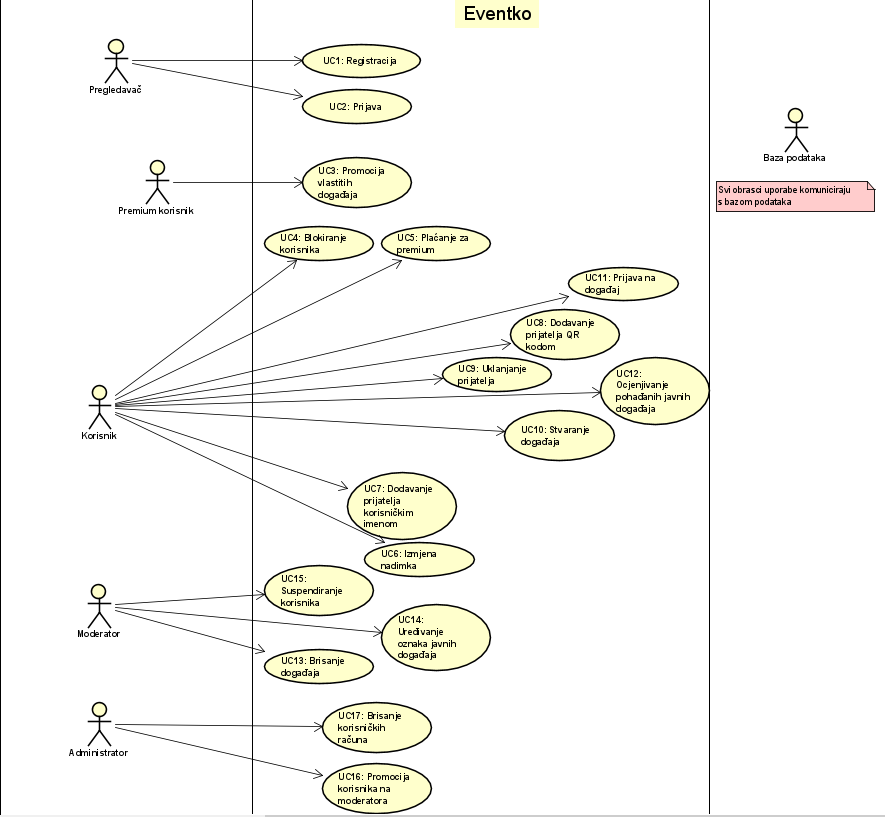
\includegraphics{slike/UseCase.jpg}
					
					
				\eject		
				
			\subsection{Sekvencijski dijagrami}
				
				\textbf{\textit{dio 1. revizije}}\\
				
			
				
				\noindent \textbf {Obrazac uporabe UC1 -Registracija}\\
				\noindent {Korisnik šalje zahtjev za prikaz Prijava stranice da bi mogao odabrati gumb za registraciju. Korisnik onda šalje zahtjev za prikaz Registracija stranice. Upisuje podatke potrebne za izradu računa koje Web aplikacija šalje bazi podataka koja radi profil. Baza vraća potvrdu nakon izrađenog profila i korisnik je vraćen na prikaz Prijava stranice.}
				
				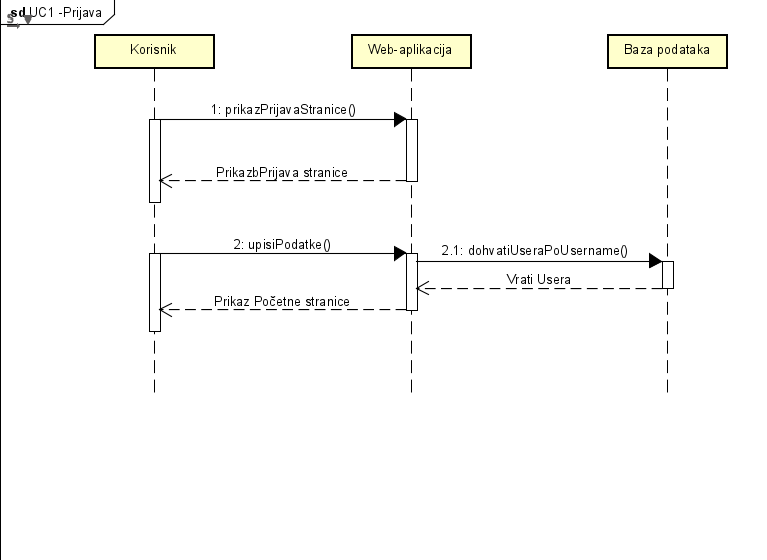
\includegraphics{slike/UC1 -Prijava}
				\eject
				
				\noindent \textbf {Obrazac uporabe UC1 -Registracija}\\
				\noindent {Korisnik šalje zahtjev za prikaz Prijava stranice nakon kojeg upisuje potrebne podatke za prijavu. Web aplikacija šalje podatke bazi podataka koja dohvaća korisnike i traži zadanog korisnika prema imenu profila. Baza podataka vraća profil korisnika nakon kojeg je korisniku prikazana Početna stranica }
				
				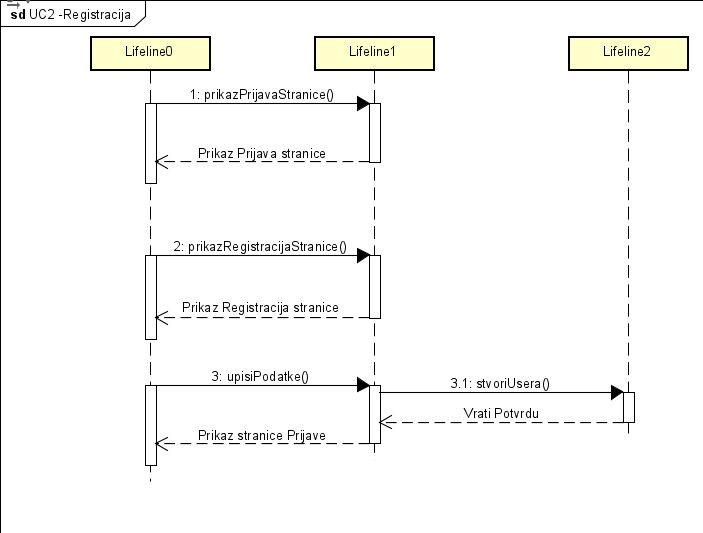
\includegraphics{slike/UC2 -Registracija.png}
				
				\eject
	
		\section{Ostali zahtjevi}
		
			\textbf{\textit{dio 1. revizije}}\\
		 
			 \textit{Nefunkcionalni zahtjevi i zahtjevi domene primjene dopunjuju funkcionalne zahtjeve. Oni opisuju \textbf{kako se sustav treba ponašati} i koja \textbf{ograničenja} treba poštivati (performanse, korisničko iskustvo, pouzdanost, standardi kvalitete, sigurnost...). Primjeri takvih zahtjeva u Vašem projektu mogu biti: podržani jezici korisničkog sučelja, vrijeme odziva, najveći mogući podržani broj korisnika, podržane web/mobilne platforme, razina zaštite (protokoli komunikacije, kriptiranje...)... Svaki takav zahtjev potrebno je navesti u jednoj ili dvije rečenice.}
			 \begin{packed_item}
			 \item  Sustav treba omogućiti rad više korisnika u stvarnom vremenu
			 \item Izvršavanje dijela programa u kojem se pristupa bazi podataka ne smije trajati duže od nekoliko sekundi
			 \item Sustav treba biti implementiran kao web aplikacija koristeći objektno-orijentirane jezike
			 \item Neispravno korištenje korisničkog sučelja ne smije narušiti funkcionalnost i rad sustava
			 \item Sustav treba biti jednostavan za korištenje, korisnici se moraju znati koristit sučeljem bez opširnih uputa
			 \item Nadogradnja sustava ne smije narušavati postojeće funkcionalnosti sustava
			 \item Veza s bazom podataka mora biti kvalitetno zaštićena, brza i otporna na vanjske greške
			 \end{packed_item}
	
	\chapter{Arhitektura i dizajn sustava}
		
	\vspace{-1cm}
	\begin{figure}[h]
		\begin{center}
			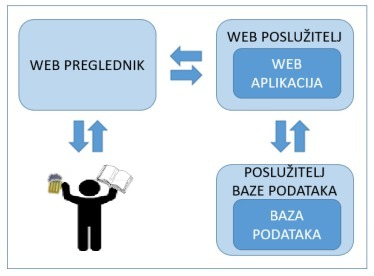
\includegraphics{slike/arhitektura_skica.png}
			\caption{Arhitektura sustava}
		\end{center}	
	\end{figure}
	
	\indent Arhitekturu tvore tri podsustava: web poslužitelj, web aplikacija te baza podataka. \textit{Web preglednik} je program za pregledavanje i navigaciju web-stranicama. Kada korisnik pošalje zahtjev za web-stranicom, preglednik dohvaća potrebne datoteke s \textit{web poslužitelja} i prikazuje stranicu na korisnikovom ekranu u namijenjenom obliku. Poslužitelj omogućuje komunikaciju klijenta s \textit{web aplikacijom} koja je na njemu pokrenuta, a prosljeđuje joj zahtjeve HTTP-om (engl. \textit{Hyper Text Transfer Protocol}). Web aplikacija odgovara na zahtjeve klijenta pristupajući po potrebi bazi podataka i vraćajući HTML dokument čitljiv u web pregledniku. \\
	
	\indent Za izradu ovog projekta koristili smo se Spring Boot frameworkom u Javi kroz razvojno okruženje IntelliJ Community Edition, Javascriptom uz React u Visual Studio Code-u te nizom drugih programa za dizajn slika i grafova (GIMP, AstahUML itd.). \\
	
	\indent Arhitektura sustava prati MVC obrazac, odnosno Model-Pogled-Nadglednik (engl. \textit{Model View Controller}), stilističku varijaciju arhitekture zasnovane na događajima. Takve arhitekture odlikuje to što se komponente međusobno ne pozivaju eksplicitno, već neke od njih generiraju signale (događaje) ne znajući koja druga "osluškuje" tj. očekuje takav signal i na njega reagira. Kod MVC-a pogodno je što smanjuje međuovisnost korisničkog sučelja i ostatka sustava, a omogućuje i nezavisan razvoj, nadogradnje i dodavanje različitih dijelova aplikacije. Sadrži različite gotove predloške za klase koji nam olakšavaju proces izrade.\\
	
	\indent MVC model sastoji se od komponenti:
	\begin{packed_item}
		\item 	\textbf{Model} - Središnja komponenta sustava, sadrži razrede čiji se objekti obrađuju. Rukuje s podatkovnom logikom i bazom podataka. Prima podatke od nadglednika.
		\item 	\textbf{Pogled} - Predstavlja model korisniku na čitljiv način. Sadrži razrede čiji objekti služe za prikaz podataka. Dinamički se osvježava.
		\item	\textbf{Nadglednik} - Razumije naputke korisnika i pretvara ih u upute ka modelu. Sadrži razrede koji upravljaju i rukuju korisničkom interakcijom s pogledom i modelom, poput poslovne logike i odgovora na događaje.
	\end{packed_item}

	\eject
		

		

				
		\section{Baza podataka}
			

		
		Za potrebe našeg sustava koristit ćemo relacijsku bazu podataka koja svojom strukturom olakšava modeliranje stvarnog svijeta. Gradivna jedinka baze je relacija, odnosno tablica koja je definirana svojim imenom i skupom atributa. Zadaća baze podataka je brza i jednostavna pohrana, izmjena i dohvat podataka za daljnju obradu. Baza podataka ove aplikacije sastoji se od sljedećih entiteta:
		
		\begin{itemize}
			\item Korisnik
			\item Uloga
			\item Vrsta
			\item Oznaka
			\item ImaUlogu
			\item JePrijatelj
			\item JeBlokiranOd
			\item Dogadjaj
			\item Pohadja
			\item ImaOznaku
			
		\end{itemize}
		
		
			\subsection{Opis tablica}
			

				
				
				\noindent\textbf{Korisnik} Ovaj entitet sadržava sve važne informacije o korisniku aplikacije. Sadrži atribute: id korisnika, nadimak, korisničko ime, email, salt, lozinka i suspendiran. Ovaj entitet u vezi je Many-to-Many s Uloga preko veze imaUlogu, u vezi Many-to-Many s Korisnik preko veze jePrijatelj, u vezi Many-to-Many s Korisnik preko veze JeBlokiranOd, te u vezi  One-to-Many s entitetom Događaj preko i u vezi Many-to-Many s entitetom Dogadjaj preko veze Pohadja.
				
				\begin{longtblr}[
					label=none,
					entry=none
					]{
						width = \textwidth,
						colspec={|X[6,l]|X[6, l]|X[20, l]|}, 
						rowhead = 1,
					} %definicija širine tablice, širine stupaca, poravnanje i broja redaka naslova tablice
					\hline \multicolumn{3}{|c|}{\textbf{Korisnik}} & tip podataka & opis varijable	 \\ \hline[3pt]
					\SetCell{LightGreen}id korisnik & BIGINT NOT NULL	&  	jedinstveni brojčani identifikator korisnika	\\ \hline
					nadimak	& VARCHAR(25) NOT NULL &   nadimak korisnika	\\ \hline
					korisnicko ime & VARCHAR(25) NOT NULL & ime korisnika  \\ \hline  
					email & VARCHAR(255) NOT NULL & email korisnika  \\ \hline 
					salt & BYTEA NOT NULL	&  salt za hashiranje lozinke		\\ \hline 
					lozinka & BYTEA NOT NULL	&  	hash lozinke	\\ \hline 
					suspendiran & BOOLEAN NOT NULL	& oznaka je li korisnik suspendiran 		\\ \hline 
					
				\end{longtblr}
			
			
				\noindent\textbf{Uloga} Ovaj entitet sadržava sve važne informacije o ulogama korisnika. Sadrži atribute: id uloga, naziv uloga i opis uloga. Ovaj entitet u vezi je Many-to-Many s Korisnik preko veze imaUlogu.
				
				\begin{longtblr}[
					label=none,
					entry=none
					]{
						width = \textwidth,
						colspec={|X[6,l]|X[6, l]|X[20, l]|}, 
						rowhead = 1,
					} %definicija širine tablice, širine stupaca, poravnanje i broja redaka naslova tablice
					\hline \multicolumn{3}{|c|}{\textbf{Uloga}}& tip podataka & opis varijable	 \\ \hline[3pt]
					\SetCell{LightGreen}id uloga & BIGINT NOT NULL	&  	jedinstveni brojčani identifikator uloge korisnika	\\ \hline
					naziv uloga	& VARCHAR(255) NOT NULL &  naziv uloge korisnika	\\ \hline 
					opis uloga & VARCHAR(255) NOT NULL & opis uloge korisnika  \\ \hline 
					
				\end{longtblr}
			
				\noindent\textbf{Vrsta} Ovaj entitet sadržava sve važne informacije o vrstama događaja. Sadrži atribute: id vrsta, naziv vrsta i opis vrsta. Ovaj entitet u vezi je Many-to-On s entitetom Dogadjaj preko identifikatora vrste u entitetu Dogadjaj.
				
				\begin{longtblr}[
					label=none,
					entry=none
					]{
						width = \textwidth,
						colspec={|X[6,l]|X[6, l]|X[20, l]|}, 
						rowhead = 1,
					} %definicija širine tablice, širine stupaca, poravnanje i broja redaka naslova tablice
					\hline \multicolumn{3}{|c|}{\textbf{Vrsta}}& tip podataka & opis varijable	 \\ \hline[3pt]
					\SetCell{LightGreen}id vrsta & INT NOT NULL	&  jedinstveni brojčani identifikator vrste događaja	\\ \hline
					naziv vrsta	& VARCHAR(255) NOT NULL &  naziv vrste događaja	\\ \hline 
					opis vrsta & VARCHAR(255) NOT NULL &  opis vrste događaja \\ \hline 
					 
				\end{longtblr}
				
				\noindent\textbf{Oznaka} Ovaj entitet sadržava sve važne informacije o oznakama događaja. Sadrži atribute: id oznaka, naziv oznaka i boja hex. Ovaj entitet u vezi je Many-to-Many s Oznaka preko veze imaOznaku.
				
				\begin{longtblr}[
					label=none,
					entry=none
					]{
						width = \textwidth,
						colspec={|X[6,l]|X[6, l]|X[20, l]|}, 
						rowhead = 1,
					} %definicija širine tablice, širine stupaca, poravnanje i broja redaka naslova tablice
					\hline \multicolumn{3}{|c|}{\textbf{Oznaka}}& tip podataka & opis varijable	 \\ \hline[3pt]
					\SetCell{LightGreen}id oznaka & INT NOT NULL	& jedinstveni brojčani identifikator oznake događaja	\\ \hline
					naziv oznaka	& VARCHAR(255) NOT NULL &  naziv oznake događaja  	\\ \hline 
					boja hex & CHAR(7) NOT NULL & boja oznake  \\ \hline 
					
				\end{longtblr}
				
				
				\noindent\textbf{ImaUlogu} Ova veza sadržava sve važne informacije po kojima saznajemo koji korisnik ima koju ulogu. Sadrži atribute: id korisnik i id uloga. Povezuje entitete Korisnik i Uloga. 
				
				\begin{longtblr}[
					label=none,
					entry=none
					]{
						width = \textwidth,
						colspec={|X[6,l]|X[6, l]|X[20, l]|}, 
						rowhead = 1,
					} %definicija širine tablice, širine stupaca, poravnanje i broja redaka naslova tablice
					\hline \multicolumn{3}{|c|}{\textbf{ImaUlogu}}& tip podataka & opis varijable	 \\ \hline[3pt]
					\SetCell{LightGreen}id korisnik & BIGINT NOT NULL	&  	jedinstveni brojčani identifikator korisnika (korisnik.id korisnik)	\\ \hline
					\SetCell{LightGreen}id uloga	& BIGINT NOT NULL &   jedinstveni brojčani identifikator uloga korisnika (uloga.id uloga)	\\ \hline 
					 
				\end{longtblr}
				
				\noindent\textbf{JePrijatelj} Ova veza sadržava sve važne informacije o tome koji je korisnik nekom drugom korisniku prijatelj. Sadrži atribute: id korisnik i id prijatelj. Povezuje entitet Korisnik sa samim sobom.
				
				\begin{longtblr}[
					label=none,
					entry=none
					]{
						width = \textwidth,
						colspec={|X[6,l]|X[6, l]|X[20, l]|}, 
						rowhead = 1,
					} %definicija širine tablice, širine stupaca, poravnanje i broja redaka naslova tablice
					\hline \multicolumn{3}{|c|}{\textbf{JePrijatelj}}	& tip podataka & opis varijable \\ \hline[3pt]
					\SetCell{LightGreen}id korisnik & BIGINT NOT NULL	&  	jedinstveni brojčani identifikator korisnika (korisnik.id korisnik)	\\ \hline
					\SetCell{LightGreen}id prijatelj	& BIGINT NOT NULL	& jedinstveni brojčani identifikator drugog korisnika prijatelja (korisnik.id korisnik)	\\ \hline 
				\end{longtblr}
			
			
				\noindent\textbf{JeBlokiranOd} Ova veza sadržava sve važne informacije o tome koji je korisnik blokiran i od kojeg je korisnika blokiran. Sadrži atribute: id blokiran i id blokiran od. Povezuje entitet Korisnik sa samim sobom.
				
				\begin{longtblr}[
					label=none,
					entry=none
					]{
						width = \textwidth,
						colspec={|X[6,l]|X[6, l]|X[20, l]|}, 
						rowhead = 1,
					} %definicija širine tablice, širine stupaca, poravnanje i broja redaka naslova tablice
					\hline \multicolumn{3}{|c|}{\textbf{JeBlokiranOd}}	& tip podataka & opis varijable \\ \hline[3pt]
					\SetCell{LightGreen}id blokiran & BIGINT NOT NULL	&  	jedinstveni brojčani identifikator korisnika koji je blokiran (korisnik.id korisnik)	\\ \hline
					\SetCell{LightGreen}id blokiran od	& BIGINT NOT NULL &   jedinstveni brojčani identifikator korisnika koji blokira (korisnik.id korisnik)	\\ \hline 
				 
				\end{longtblr}
				
				
				\noindent\textbf{Dogadjaj} Ovaj entitet sadržava sve važne informacije o događaju. Sadrži atribute: id događaj, naziv, mjesto, vrijeme početka, vrijeme kraja, opis, promoviran, koordinate, id organizator i id vrsta. Ovaj entitet u vezi je Many-to-One s entitetom Vrsta preko identifikatora vrste, u vezi Many-to-One s entitetom Korisnik preko identifikatora korisnika, u vezi Many-to-Many s entitetom Korisnik preko veze Pohadja i u vezi Many-to-Many s Oznaka preko veze imaOznaku.
				
				\begin{longtblr}[
					label=none,
					entry=none
					]{
						width = \textwidth,
						colspec={|X[6,l]|X[6, l]|X[20, l]|}, 
						rowhead = 1,
					} %definicija širine tablice, širine stupaca, poravnanje i broja redaka naslova tablice
					\hline \multicolumn{3}{|c|}{\textbf{Dogadjaj}}	& tip podataka & opis varijable \\ \hline[3pt]
					\SetCell{LightGreen}id dogadjaj & BIGINT NOT NULL	&  	jedinstveni brojčani identifikator događaja  	\\ \hline
					naziv	& VARCHAR(255) NOT NULL & naziv događaja  	\\ \hline 
					mjesto & VARCHAR(255) NOT NULL & mjesto zbivanja događaja  \\ \hline 
					vrijeme poc & TIMESTAMP NOT NULL	& vrijeme počinjanja događaja 		\\ \hline 
					vrijeme kraj & TIMESTAMP NOT NULL	&  	vrijeme završetka događaja	\\ \hline
					opis & VARCHAR(255) NOT NULL & opis događaja \\ \hline
					promoviran & BOOLEAN NOT NULL &  oznaka je li događaj promoviran \\ \hline 
					koordinate & VARCHAR(255) NOT NULL & koordinate događaja \\ \hline
					\SetCell{LightBlue}id organizator & BIGINT NOT NULL &   jedinstveni brojčani identifikator organizatora događaja (korisnik.id korisnik) \\ \hline 
					\SetCell{LightBlue}id vrsta & INT NOT NULL & jedinstveni brojčani identifikator vrste događaja (vrsta.id vrsta)
					\\ \hline
				\end{longtblr}
				
				
				\noindent\textbf{Pohadja} Ova veza sadržava sve važne informacije o tome tko je pohađao koji događaj i kako ga je ocijenio. Sadrži atribute: recenzija, id polaznika i id događaja. Povezuje entitete Korisnik i Dogadjaj.
				
				\begin{longtblr}[
					label=none,
					entry=none
					]{
						width = \textwidth,
						colspec={|X[6,l]|X[6, l]|X[20, l]|}, 
						rowhead = 1,
					} %definicija širine tablice, širine stupaca, poravnanje i broja redaka naslova tablice
					\hline \multicolumn{3}{|c|}{\textbf{Pohadja}}	& tip podataka & opis varijable \\ \hline[3pt]
					recenzija & SMALLINT NOT NULL	&  recenzija korisnika za događaj	\\ \hline
				    \SetCell{LightGreen} id pohadjatelja	& BIGINT NOT NULL &  jedinstveni brojčani identifikator pohađatelja (korisnik.id korisnik)	\\ \hline 
					\SetCell{LightGreen} id dogadjaja & BIGINT NOT NULL &  jedinstveni brojčani identifikator događaja (dogadjaj.id dogadjaj) \\ \hline 
					 
				\end{longtblr}
			
				
				\noindent\textbf{ImaOznaku} Ovaa veza sadržava sve važne informacije o oznakama određenih događaja. Sadrži atribute: id događaj i id oznaka. Povezuje entitete Oznaka i Dogadajaj.
				
				\begin{longtblr}[
					label=none,
					entry=none
					]{
						width = \textwidth,
						colspec={|X[6,l]|X[6, l]|X[20, l]|}, 
						rowhead = 1,
					} %definicija širine tablice, širine stupaca, poravnanje i broja redaka naslova tablice
					\hline \multicolumn{3}{|c|}{\textbf{ImaOznaku}}	& tip podataka & opis varijable \\ \hline[3pt]
					\SetCell{LightGreen}id dogadjaj & BIGINT NOT NULL	&  	jedinstveni brojčani identifikator događaja (dogadjaj.id dogadjaj)	\\ \hline
					\SetCell{LightGreen}id oznaka	& INT NOT NULL &   jedinstveni brojčani identifikator oznake (oznaka.id oznaka)	\\ \hline 
				
				\end{longtblr}
			
				
			
			
				
				
			
			\subsection{Dijagrami baze podataka}
				
			\begin{figure}[h]
				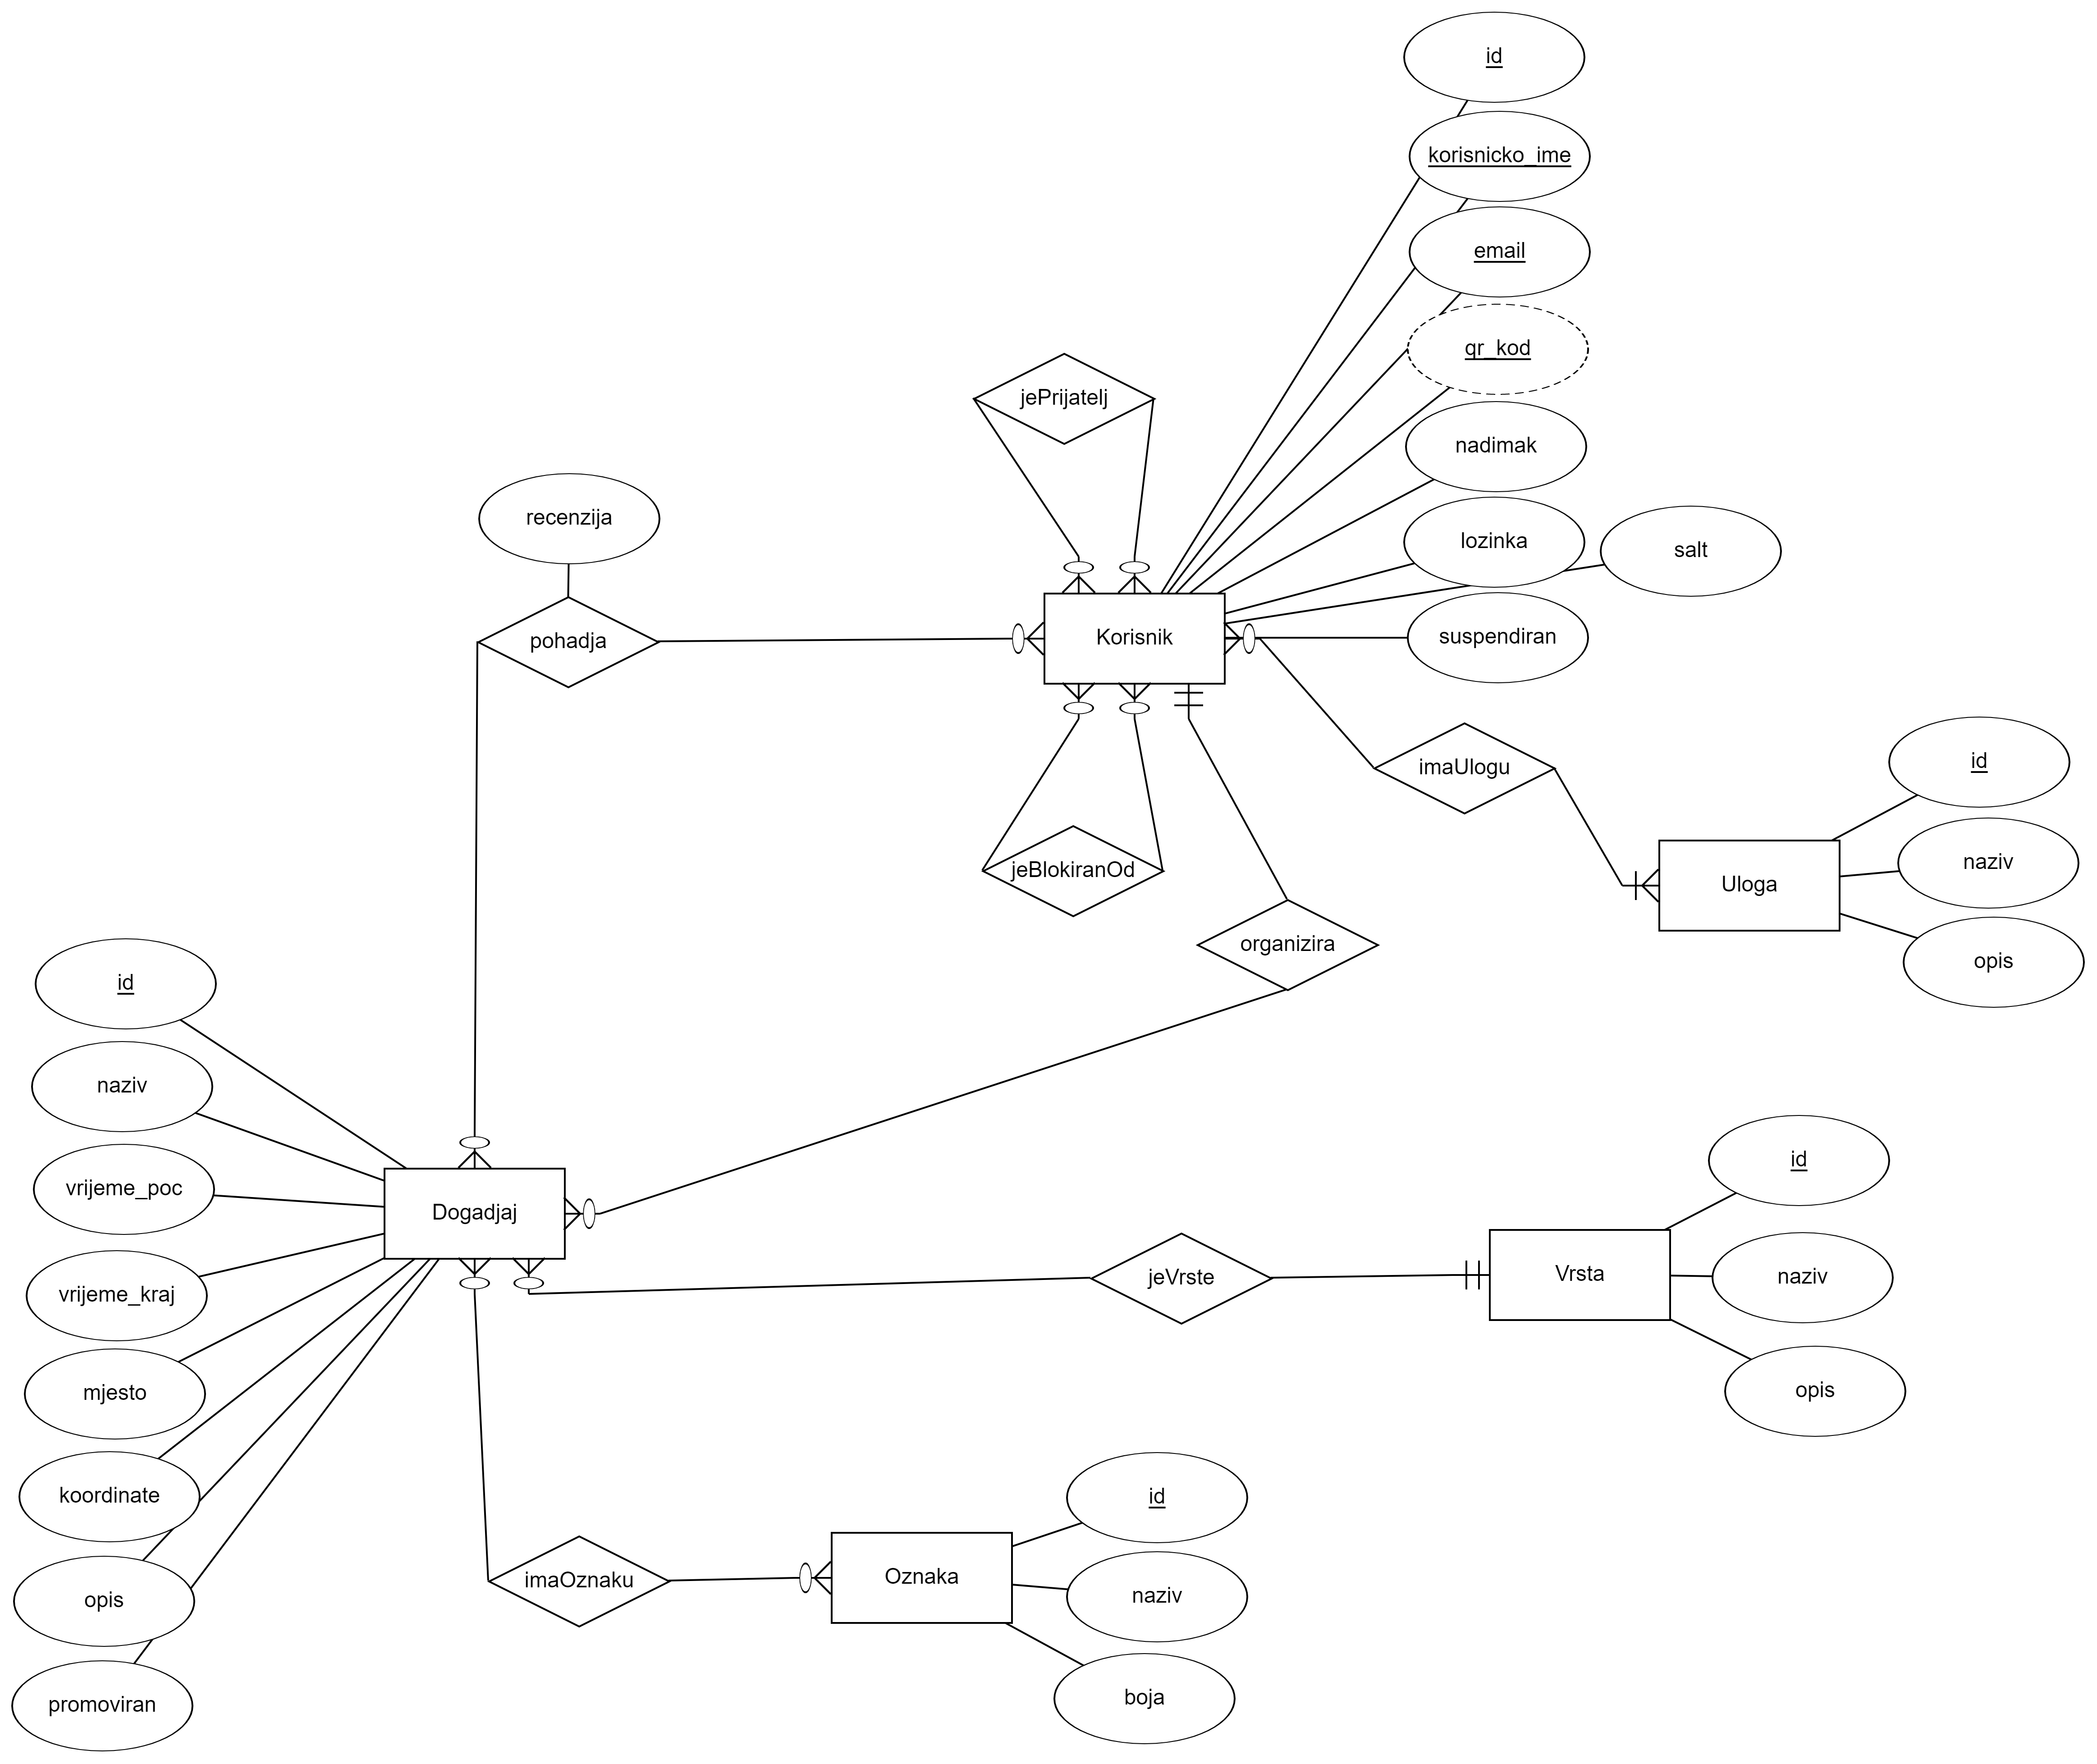
\includegraphics[width=\textwidth]{dijagrami/Baza podataka/ER model.png}
				\caption{ER dijagram baze podataka}
			\end{figure}
				
			\newpage
			\vfill	
			
			\begin{figure}[h]
				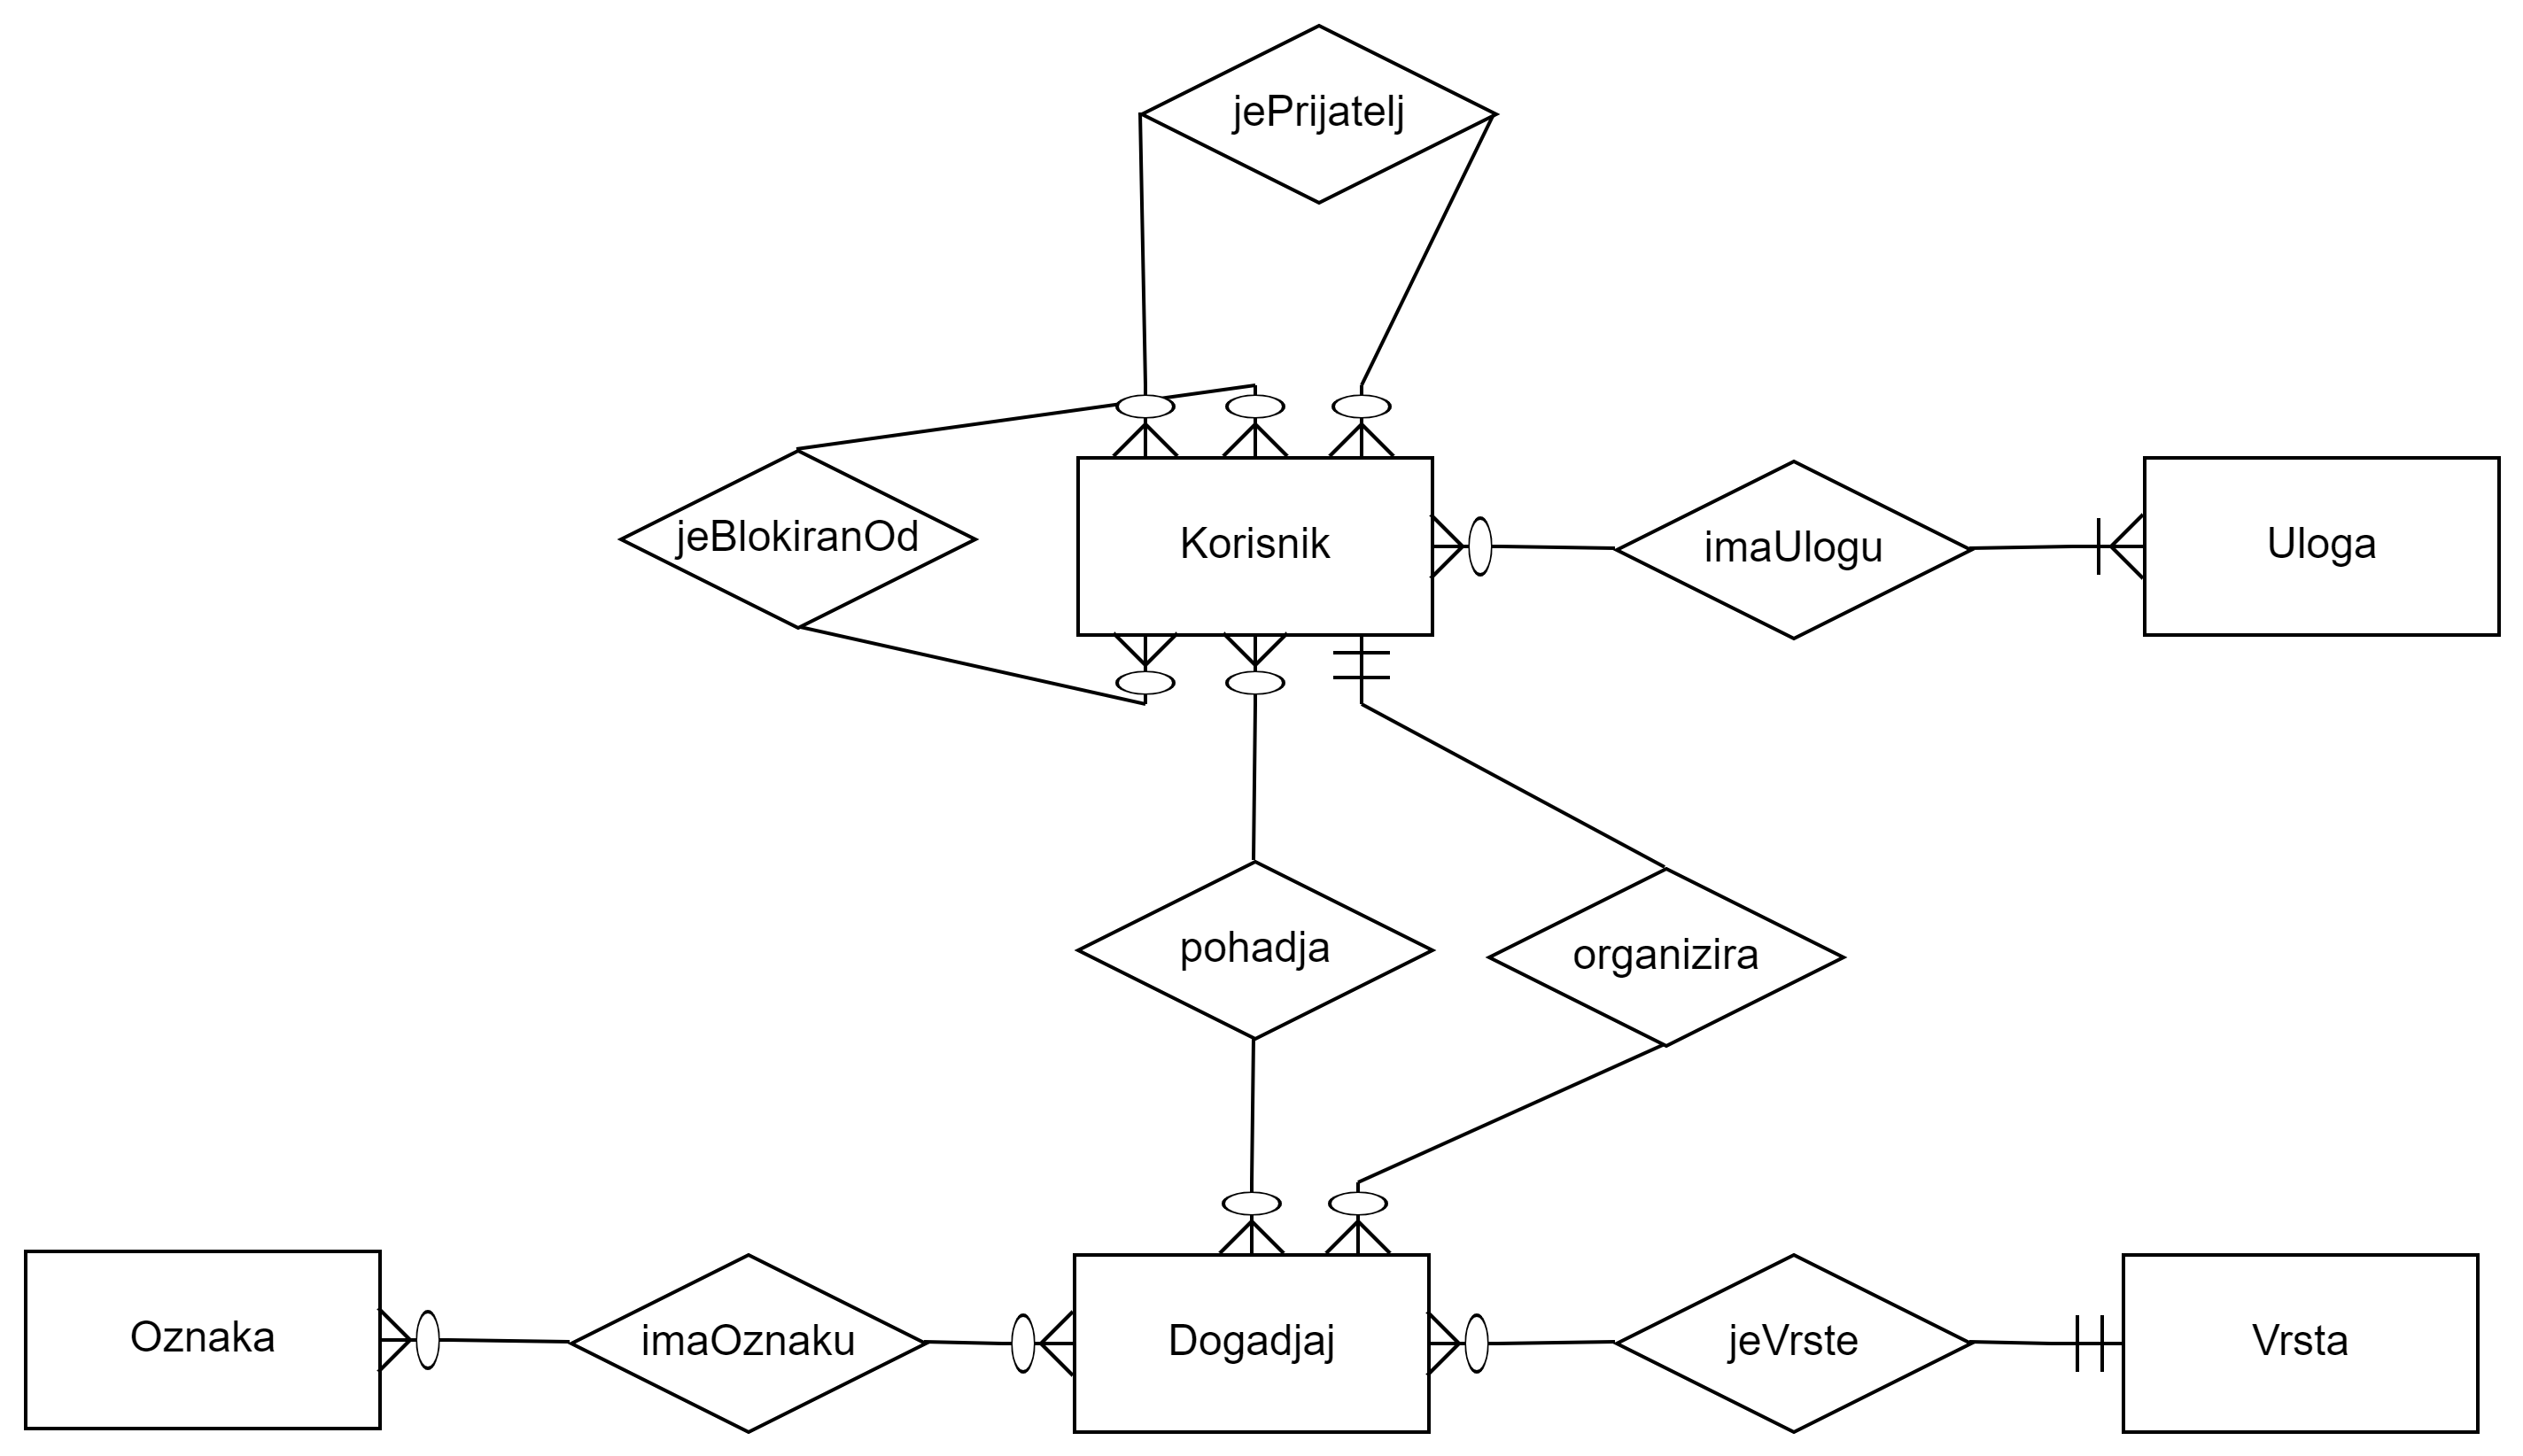
\includegraphics[width=\textwidth]{dijagrami/Baza podataka/ER model (bez atributa).png}
				\caption{ER dijagram baze podataka bez atributa}
			\end{figure}
				
			\begin{figure}[H]
				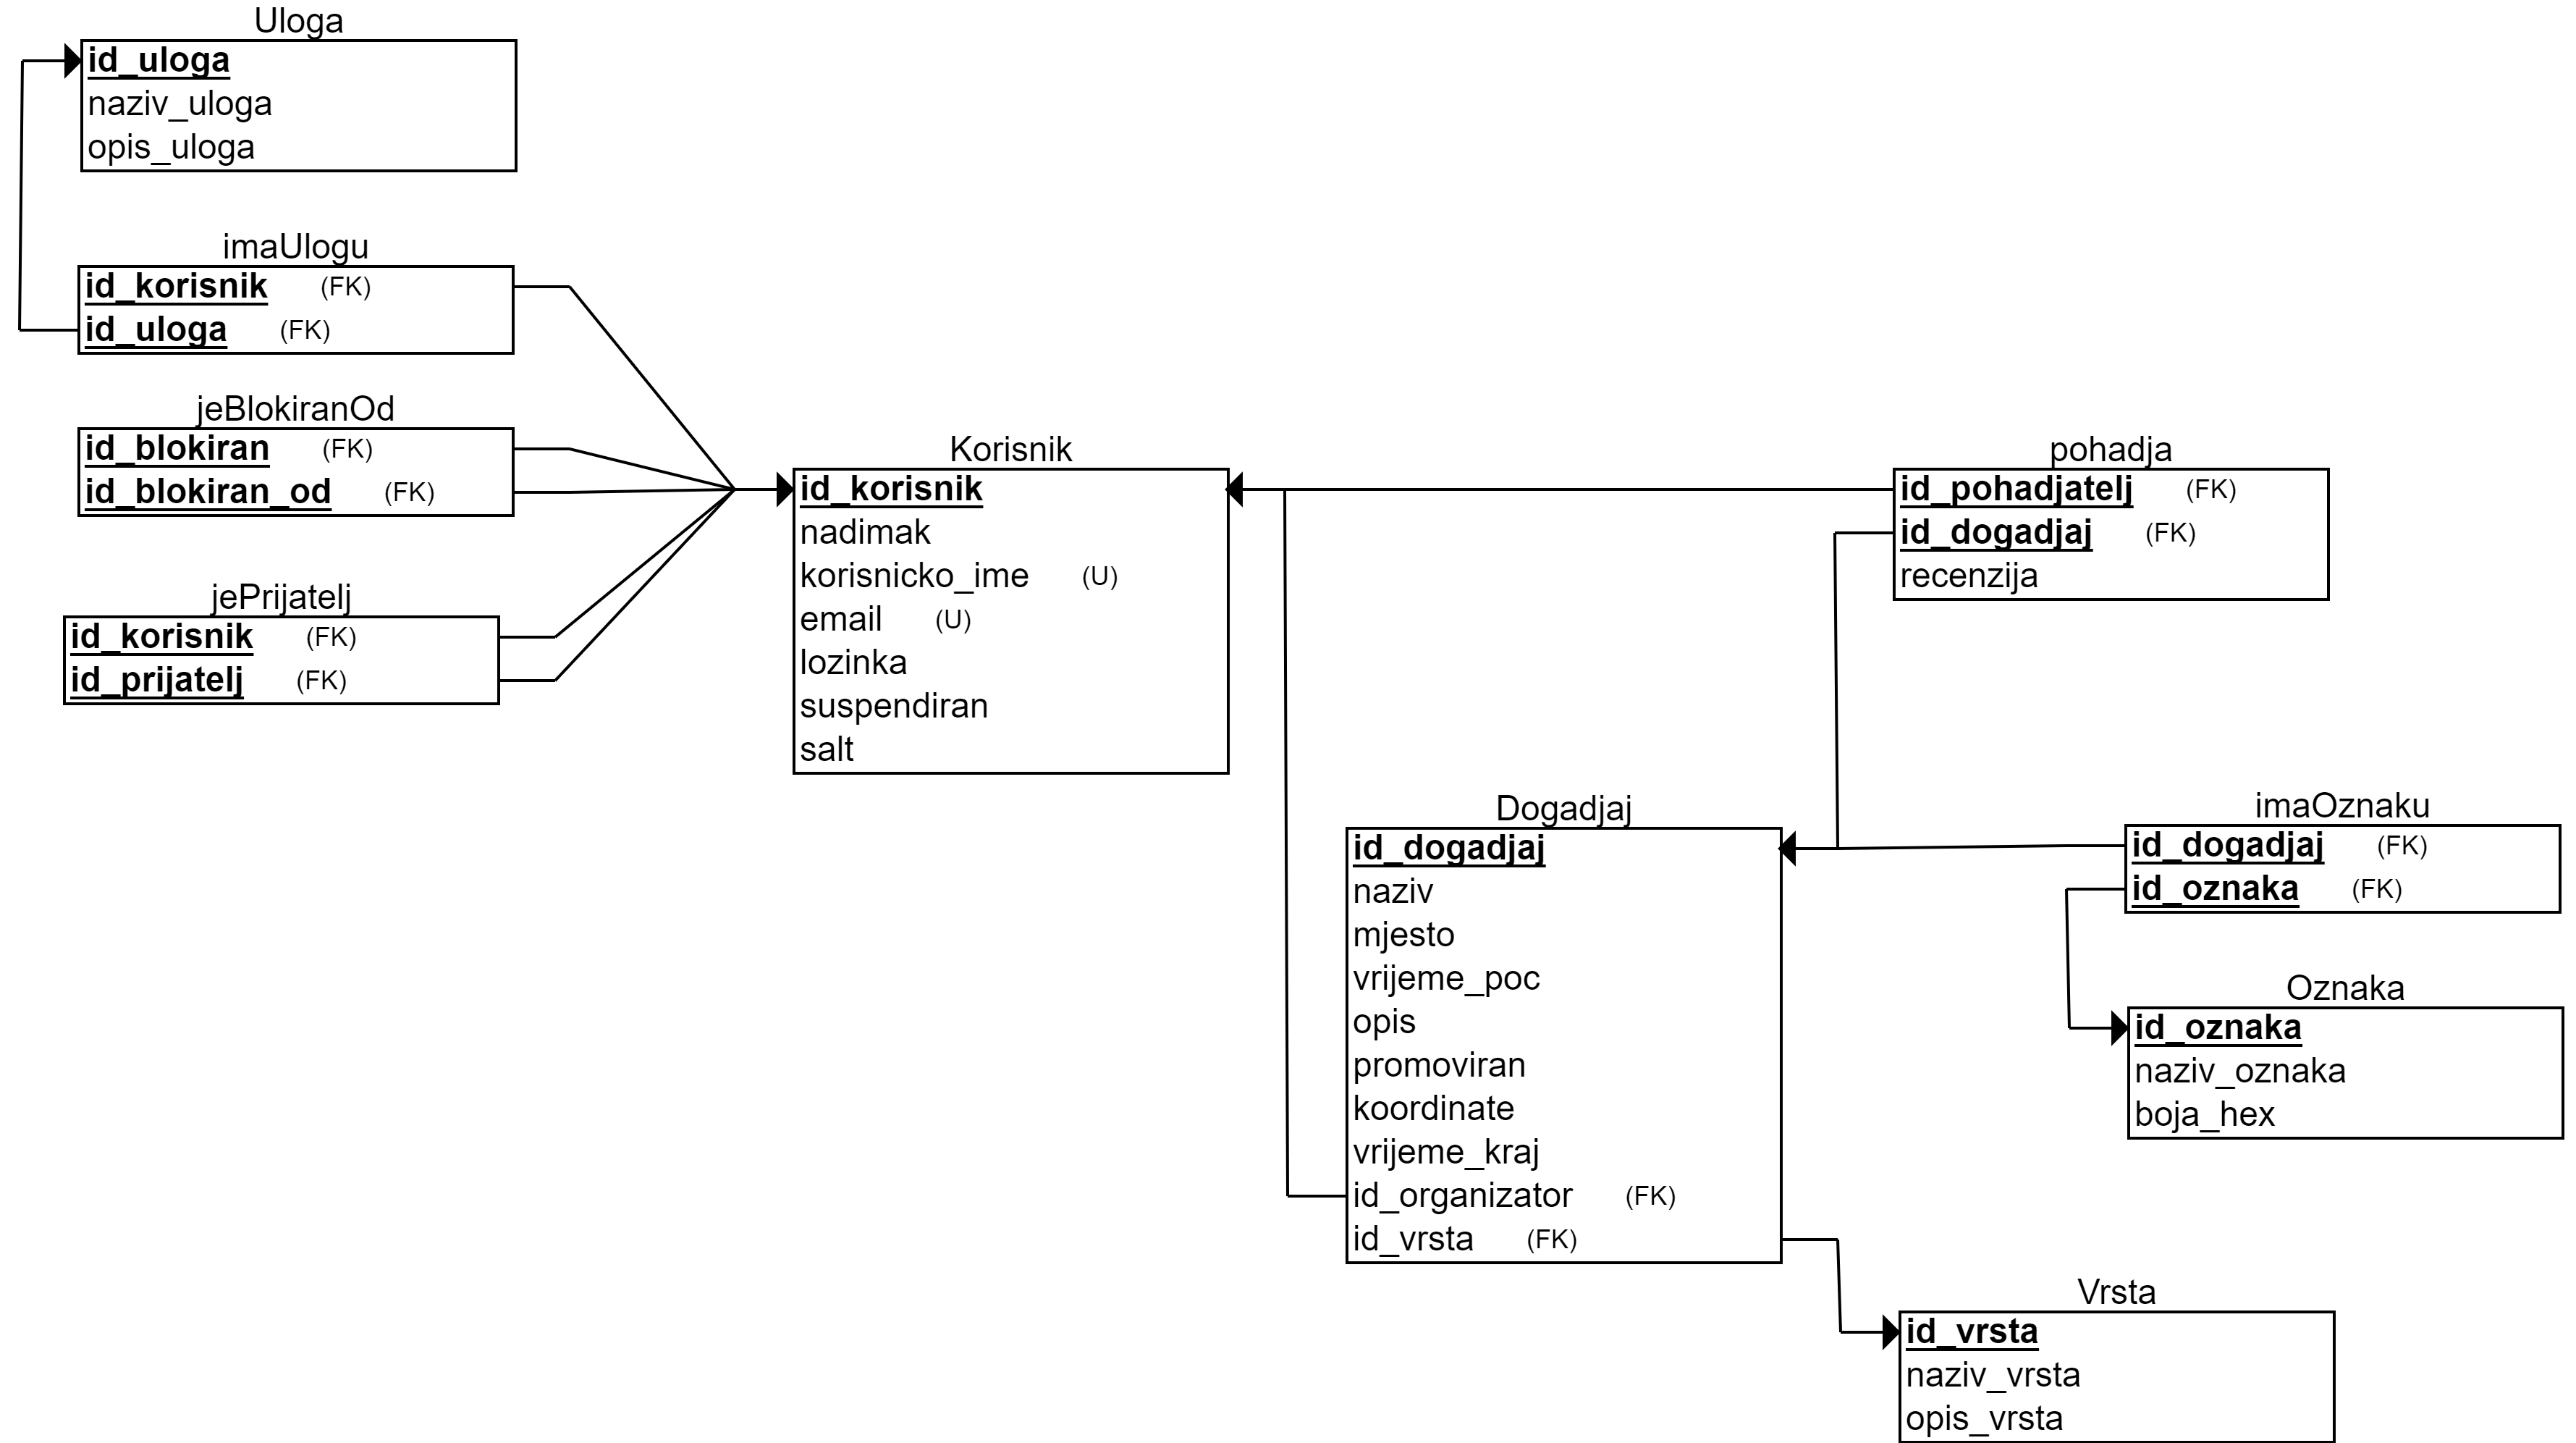
\includegraphics[width=\textwidth]{dijagrami/Baza podataka/REL shema.png}
				\caption{Relacijski dijagram baze podataka}
			\end{figure}
				
			\vfill
			\clearpage
			
			\eject
			
			
		\section{Dijagram razreda}
			
			\indent Na naredne tri slike nalaze se dijagrami razreda podijeljeni logički po srodnosti. Neki razredi povezani su i s onima na odvojenim slikama što se da zaključiti po nazivima njihovih metoda. \\
			
			\indent Razredi na slici 4.6 u gornjem redu su kontroleri. Njihove metode služe za primanje i slanje DTO-ova (\textit{Data Transfer Objects}) prema frontendu u obliku JSON datoteka s html statusnim kodom. Pozivaju funkcije servisa. Razlikuju se kontroleri za korisnike, događaje te postupke prijave i registracije. Sami DTO razredi nalaze se na slici 4.5, a to su zahtjevi i odgovori za prijavu i registraciju. \\
			
			\indent Razredi na slici 4.6 u sredini su servisi. Služe za komunikaciju između repozitorija i kontrolera. \\
			
			\indent Razredi na slici 4.6 u donjem redu su repozitoriji. Služe za pozivanje SQL upita nad bazom podataka. \\
			
			\indent Razredi na slici 4.7 su modeli. Modeliraju potrebne razrede iz baze podataka. Razred \textit{User} predstavlja korisnika aplikacije, \textit{Role} predstavlja različite uloge, \textit{Event} događaje, \textit{EventType} vrste događaja i \textit{Tag} oznake za događaje.
			
			
			\begin{figure}[h]
				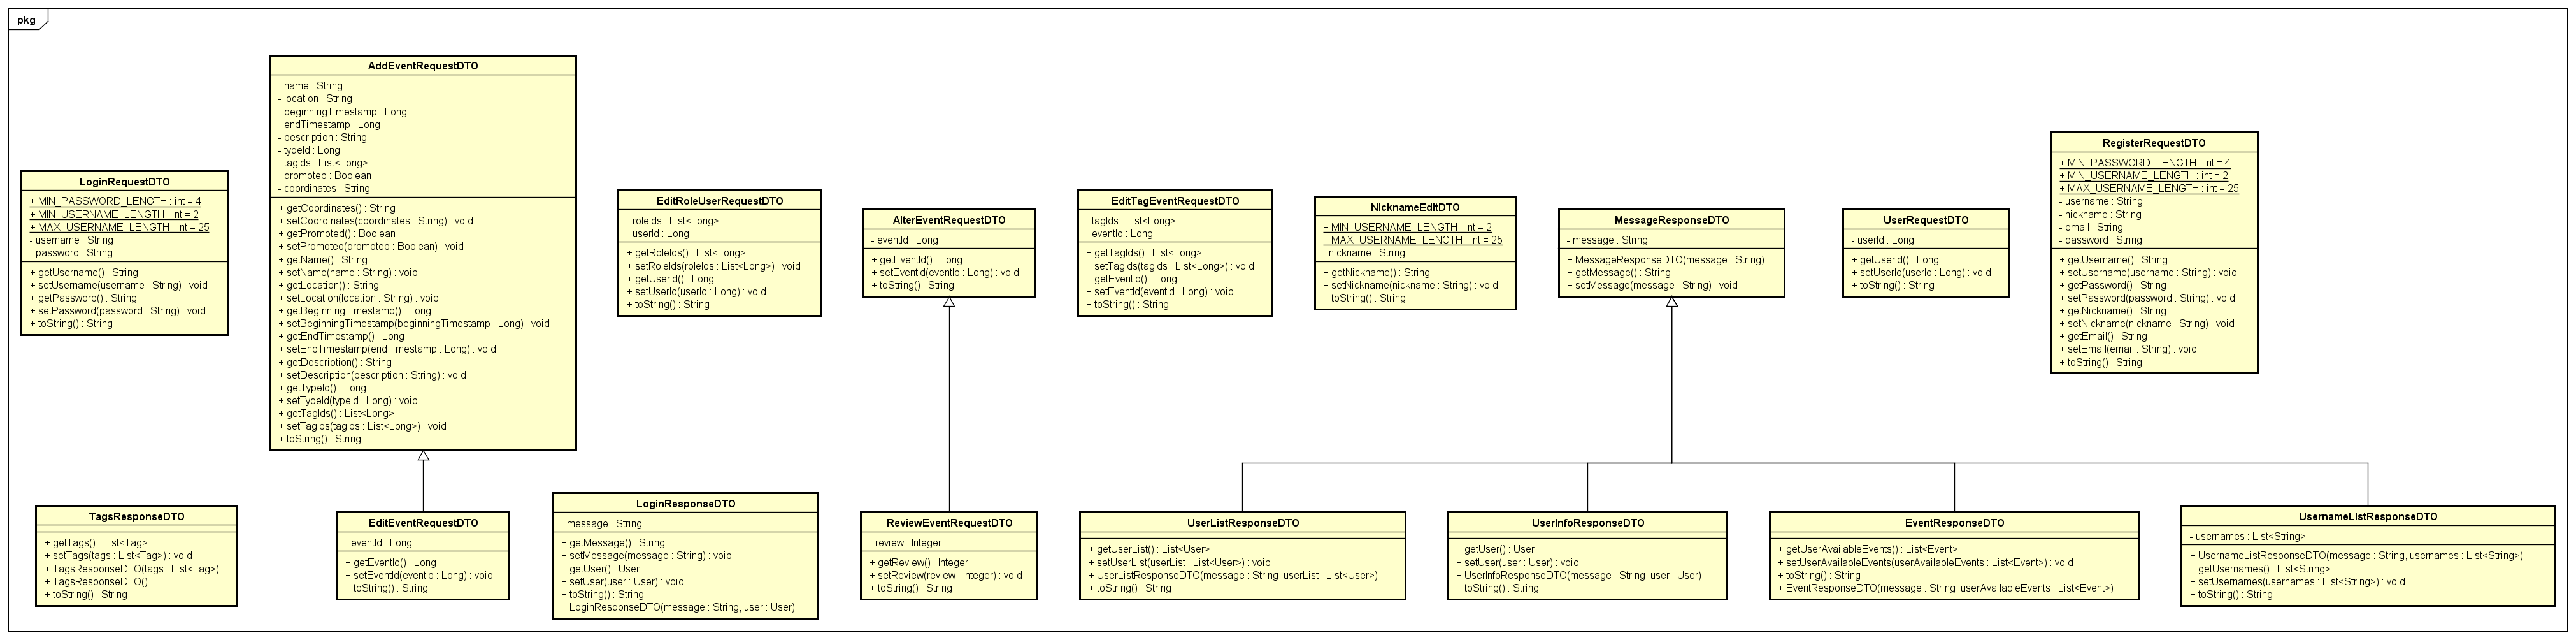
\includegraphics[width=\textwidth]{dijagrami/RAZREDNI - DTO dijagram.png}
				\caption{Dijagram razreda - DTO-ovi}
			\end{figure}
		
		    \begin{figure}[H]
		    	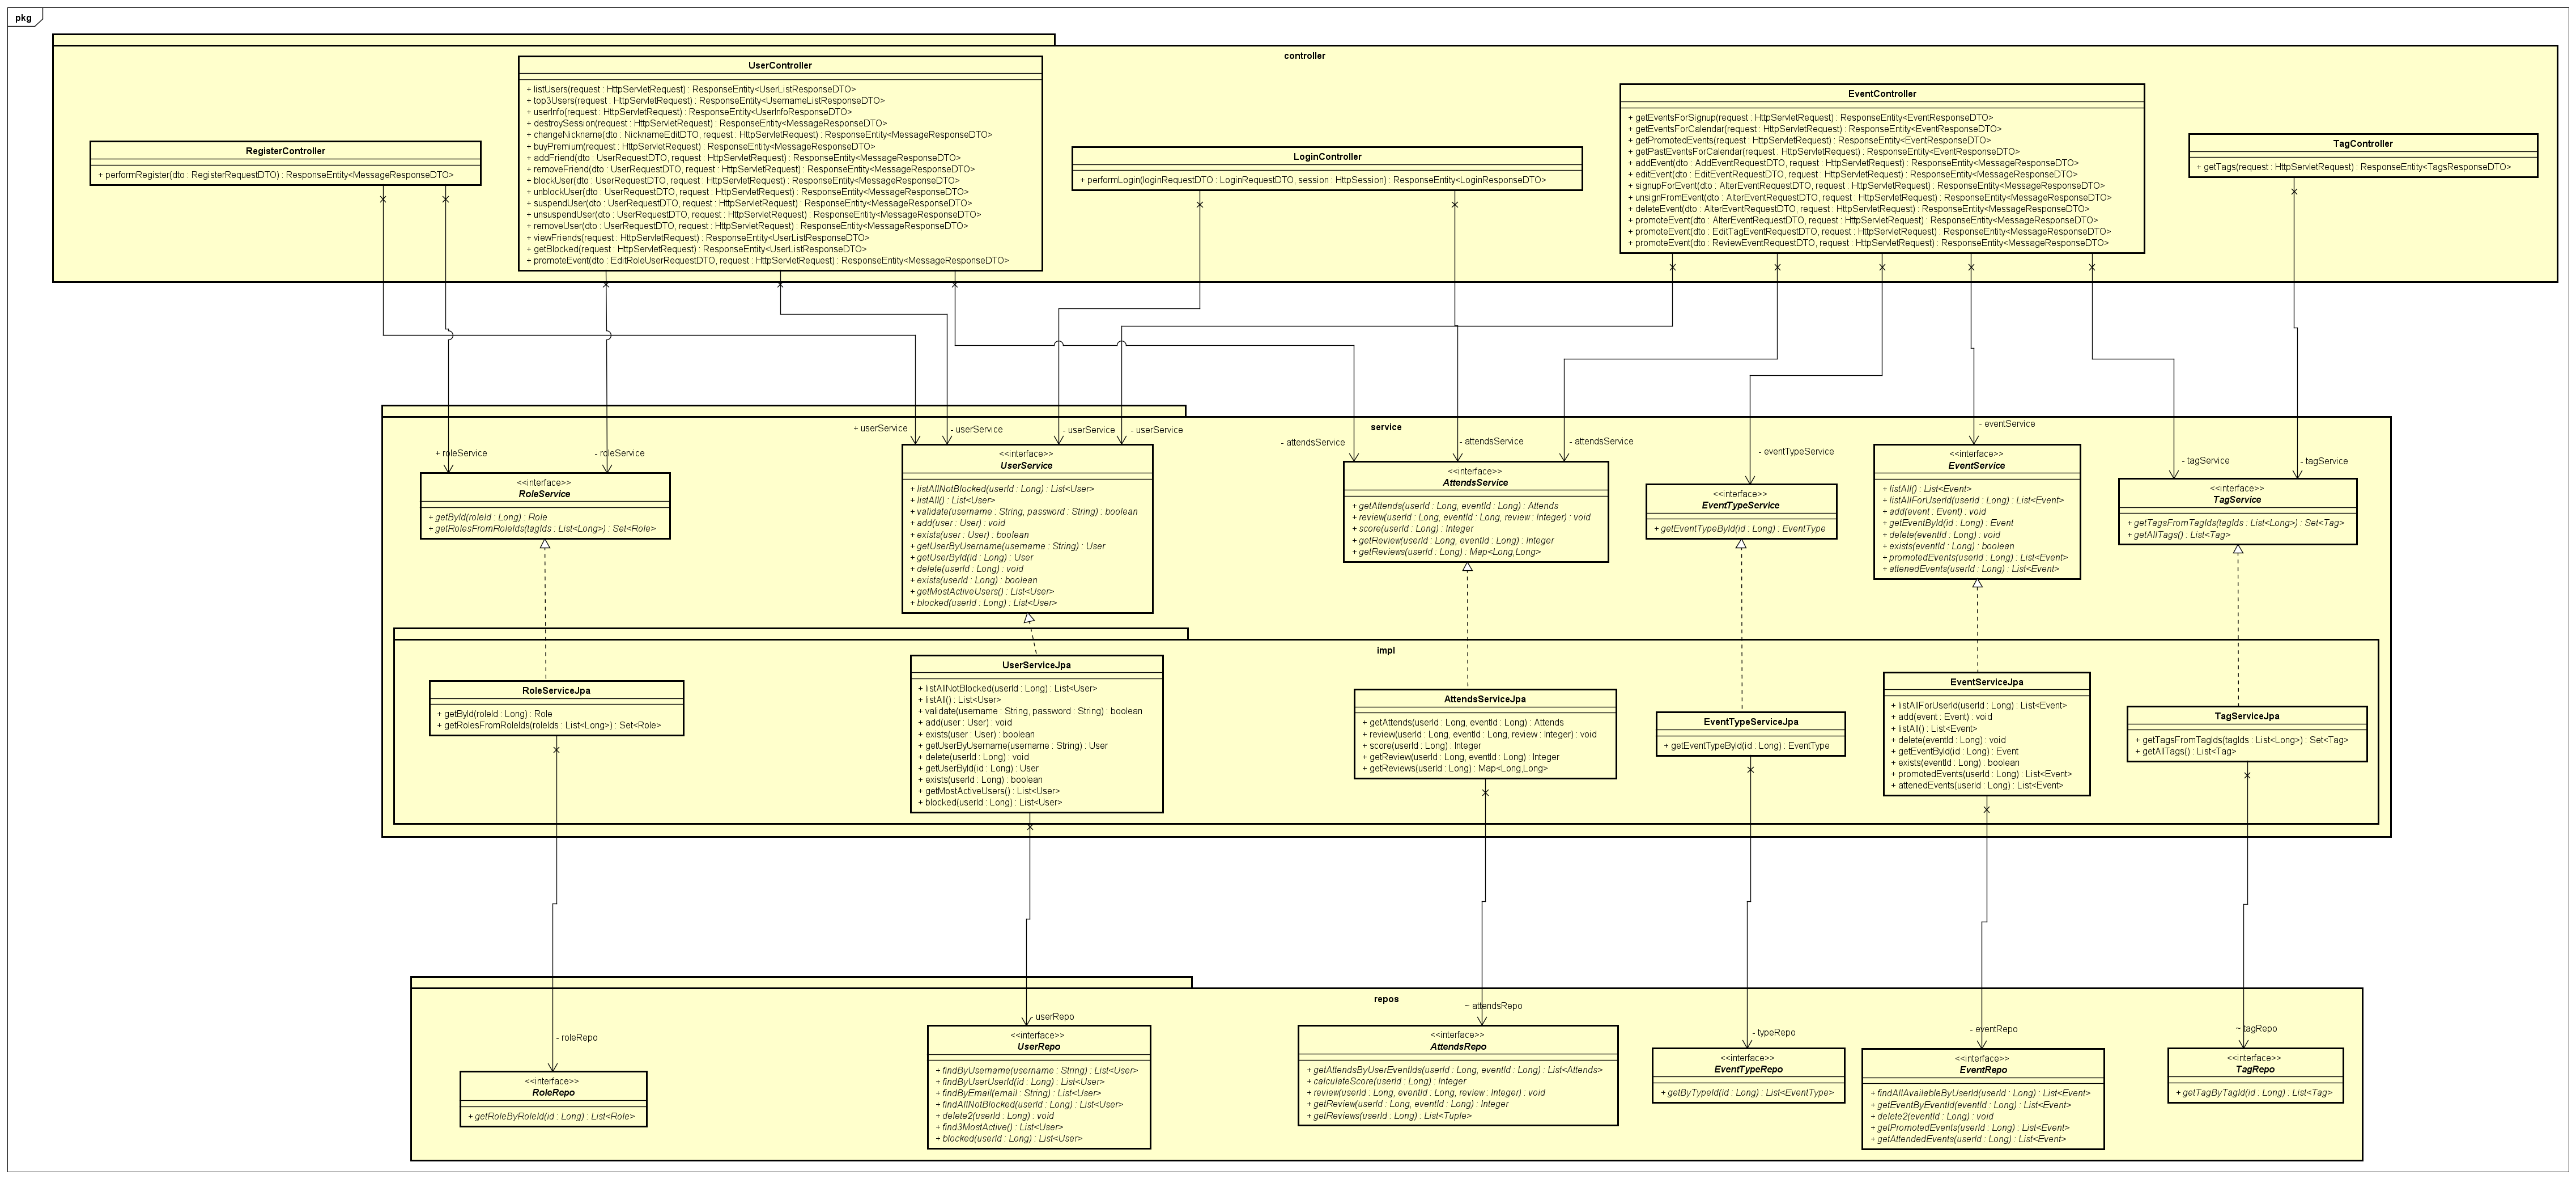
\includegraphics[width=\textwidth]{dijagrami/RAZREDNI - Controller - Service - Repo.png}
		    	\caption{Dijagram razreda - kontroleri, servisi i repozitoriji}
		    \end{figure}
			
			\begin{figure}[H]
				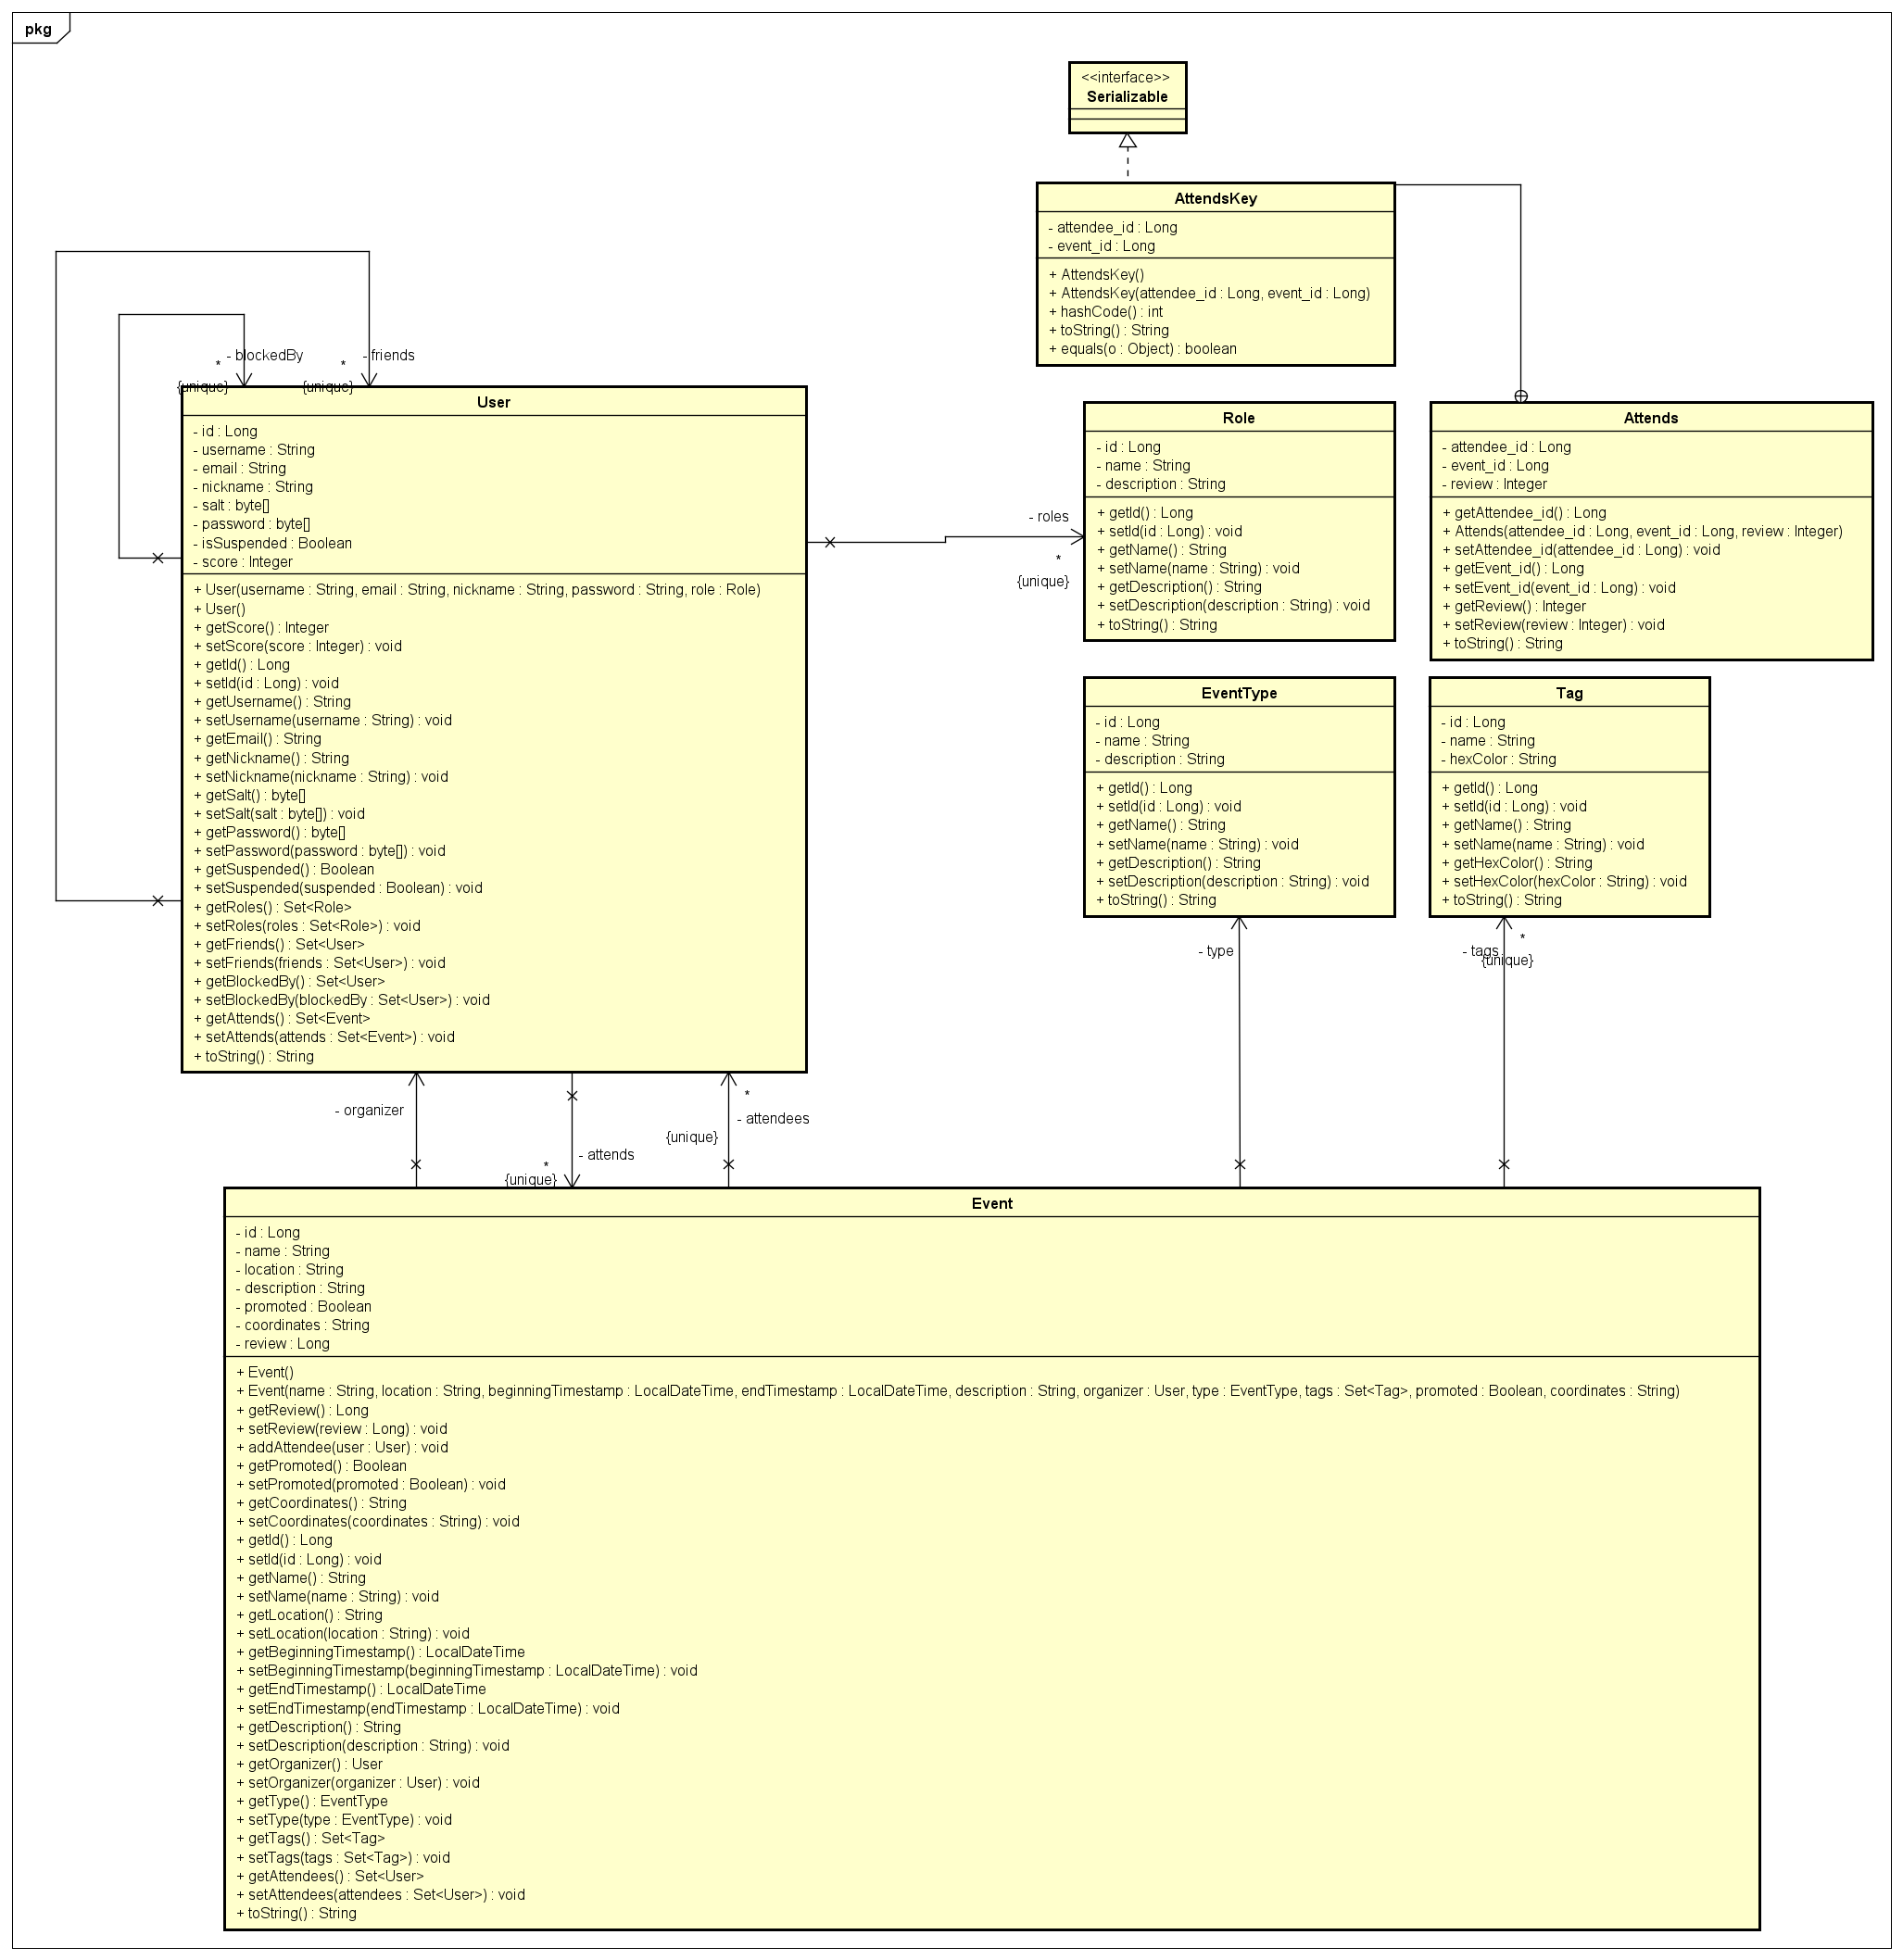
\includegraphics[width=\textwidth]{dijagrami/RAZREDNI - Dijagram modela.png}
				\caption{Dijagram razreda - modeli}
			\end{figure}
		
			\eject

		
			\section{Dijagram stanja}
			
				\begin{figure}[H]
					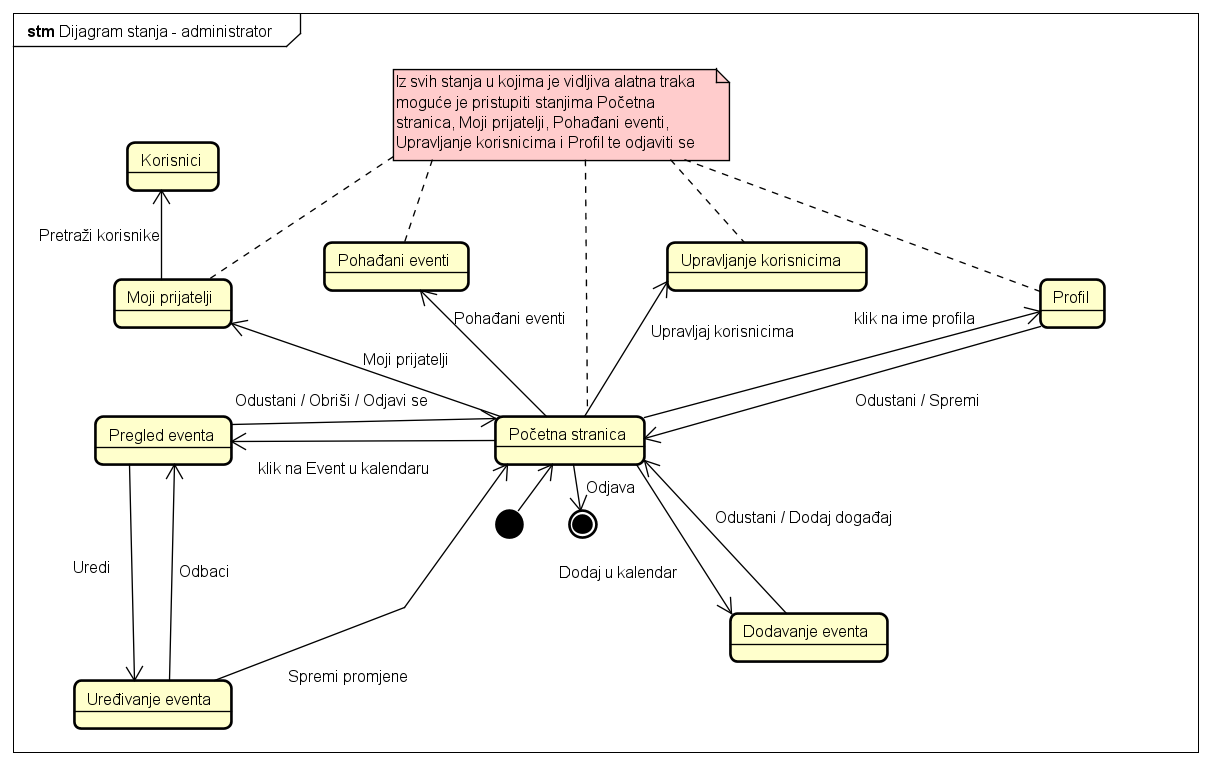
\includegraphics[width=\textwidth]{dijagrami/Dijagram stanja - administrator.png}
					\caption{Dijagram stanja}
				\end{figure}

				\indent Dijagram stanja opisuje dinamičko ponašanje sustava uslijed raznih mogućih događaja. Uspješnom prijavom prikazana je početna stranica s kalendarom s koje preko alatne trake možemo pristupiti stranicama Moji prijatelji, Pohađani eventi, Upravljanje korisnicima (samo moderator i administrator) te vlastitom korisničkom profilu. Klik na \textit{eventko} logotip uvijek vraća na početnu stranicu. Opcija \textit{Dodaj u kalendar} otvara izbornik za stvaranje novog eventa, a postojeće evente moguće je klikom na njih u kalendaru pregledavati i uređivati.
			
				\eject 
		
			\section{Dijagram aktivnosti}
			
				\begin{figure}[H]
					\includegraphics[height=0.85\textheight]{dijagrami/Dijagram aktivnosti - stvaranje događaja.png}
					\caption{Dijagram aktivnosti za stvaranje novog događaja}
				\end{figure}
			
				\indent Dijagramom aktivnosti modeliran je tijek zadataka i poslova pri korisnikovom stvaranju novog događaja. Format podataka koji se provjerava na frontendu mora sadržavati stavke \textit{name, location, beginningTimestamp, endTimeStamp, description, typeId, tagIds}, svi podaci moraju biti predviđenog tipa, a \textit{typeId} mora biti 1, 2 ili 3. Ukoliko je korisnik trenutno suspendiran, a pokušava stvoriti javni događaj, to će mu biti onemogućeno. Vremenska ograničenja provjeravaju se na backendu i automatski na bazi podataka kako ne bi bilo moguće stvoriti događaj u prošlosti niti postaviti datum i vrijeme početka nakon datuma i vremena završetka. Ukoliko su sve provjere uspješne događaj se stvara u bazi podataka, a korisniku se pokazuje ažurirana početna stranica s njegovim novim događajem upisanim u kalendar.
			
				\eject
				
			\section{Dijagram komponenti}
		
				\textbf{\textit{dio 2. revizije}}\\
		
			 	\textit{Potrebno je priložiti dijagram komponenti s pripadajućim opisom. Dijagram komponenti treba prikazivati strukturu cijele aplikacije.}
	\chapter{Implementacija i korisničko sučelje}
		
		
		\section{Korištene tehnologije i alati}
		
			\indent U izradi projekta većina digitalne komunikacije ostvarena je preko platformi WhatsApp (https://web.whatsapp.com/) i Discord (https://discord.com/). Korištene su sljedeće tehnologije i alati:
			
			\begin{itemize}
				\item \textbf{Springboot}
				\begin{itemize}
					\item open source radni okvir za kreaciju mikro-servisa, savršen za naše potrebe
					\item u njemu je izrađen backend dio projekta
					\item https://spring.io/projects/spring-boot
				\end{itemize}
				
				\item \textbf{React}
				\begin{itemize}
					\item JavaScript biblioteka za izgradnju korisničkih sučelja
					\item korišten za izradu čitavog frontenda dijela aplikacije s kojim korisnik dolazi u interakciju
					\item provjerava ispravnost podataka unesenih u obrasce
					\item https://www.reactjs.org/
				\end{itemize}
				
				\item \textbf{PostgreSQL}
				\begin{itemize}
					\item jezik u kojem je napravljena baza podataka
					\item besplatan i open source sustav za upravljanje relacijskim bazama podataka s naglaskom na mogućnosti proširivanja
					\item https://www.postgresql.org/
				\end{itemize}
			
				\item \textbf{pgAdmin}
				\begin{itemize}
					\item za upravljanje bazom podataka neovisno o backendu
					\item https://www.pgadmin.org/
				\end{itemize}
			
				\item \textbf{IntelliJ}
				\begin{itemize}
					\item IDE za javu u kojem je kodiran backend dio projekta
					\item https://www.jetbrains.com/idea/
				\end{itemize}
			
				\item \textbf{Postman}
				\begin{itemize}
					\item platforma pomoću koje su testirane backend API poveznice
					\item https://www.postman.com/
				\end{itemize}
			
				\item \textbf{Render}
				\begin{itemize}
					\item cloud platforma za izradu i besplatno hostanje web-aplikacija i stranica
					\item korišten za puštanje backenda u pogon i hostanje baze podataka
					\item https://www.render.com/
				\end{itemize}
				
				\item \textbf{Vercel}
				\begin{itemize}
					\item cloud platforma za besplatno hostanje web-stranica i servisa
					\item korišten za puštanje frontenda u pogon
					\item https://www.vercel.com/
				\end{itemize}
			
				\item \textbf{GIMP 2.10}
				\begin{itemize}
					\item uređivač slika u kojem je dizajniran logotip aplikacije i pojedini grafički prikazi u dokumentaciji
					\item https://www.gimp.org/
				\end{itemize}	
			
				\item \textbf{TeXstudio}
				\begin{itemize}
					\item integrirani uređivač za LaTeX
					\item u njemu je napisana čitava projektna dokumentacija
					\item https://www.texstudio.org/
				\end{itemize}
			
				\item \textbf{TeX Live}
				\begin{itemize}
					\item softverska distribucija za TeX s mnogobrojnim paketima i fontovima
					\item https://www.tug.org/texlive/
				\end{itemize}
			
				\item \textbf{Astah UML}
				\begin{itemize}
					\item program za uređivanje svih vrsta UML dijagrama
					\item svi dijagrami u ovom dokumentu načinjeni su u Astahu
					\item https://astah.net/products/astah-uml/
				\end{itemize}
			
				\item \textbf{GitLab}
				\begin{itemize}
					\item stranica za funkcionalno zajedničko stvaranje i uređivanje grupnog projekta
					\item https://about.gitlab.com
				\end{itemize}
			
				\item \textbf{Selenium}
				\begin{itemize}
					\item program za automatizaciju web aplikacija u svrhe testiranja
					\item korištena za testove u sljedećem poglavlju (5.2)
					\item https://www.selenium.dev
				\end{itemize}
			
				\item \textbf{Visual Studio Code}
				\begin{itemize}
					\item uređivač izvornog koda za razne programske jezike
					\item https://code.visualstudio.com/
				\end{itemize}
			\end{itemize}
			
			\eject 
		
	
		\section{Ispitivanje programskog rješenja}
			
			\textbf{\textit{dio 2. revizije}}\\
			
			 \textit{U ovom poglavlju je potrebno opisati provedbu ispitivanja implementiranih funkcionalnosti na razini komponenti i na razini cijelog sustava s prikazom odabranih ispitnih slučajeva. Studenti trebaju ispitati temeljnu funkcionalnost i rubne uvjete.}
	
			
			\subsection{Ispitivanje komponenti}
			\textit{Potrebno je provesti ispitivanje jedinica (engl. unit testing) nad razredima koji implementiraju temeljne funkcionalnosti. Razraditi \textbf{minimalno 6 ispitnih slučajeva} u kojima će se ispitati redovni slučajevi, rubni uvjeti te izazivanje pogreške (engl. exception throwing). Poželjno je stvoriti i ispitni slučaj koji koristi funkcionalnosti koje nisu implementirane. Potrebno je priložiti izvorni kôd svih ispitnih slučajeva te prikaz rezultata izvođenja ispita u razvojnom okruženju (prolaz/pad ispita). }
			
			
			
			
			
			\subsection{Ispitivanje sustava}
			
			 
			 
		 	
		 	\indent U nastavku su priloženi testovi za ispitivanje sustava u radnom okviru Selenium. Testni slučajevi su napravljeni uz pomoć dodatka za preglednik Selenium IDE. Provedeni su testovi za točnu registraciju, krivu prijavu, odjavu sa profila, dodavanje događaja, te adminove mogućnosti suspendiranja i odsuspendiranja korisnika.
		 	
		 	\indent Za test točne registracije koriste se ulazni podaci "registracija1" za korisničko ime, "registracija1" za nadimak, "registracija1@gmail.com" za e-mail, te "registracija1" za lozinku i ponovljenu lozinku(prije registracije ne postoji korisnik sa istim podacima). Nakon toga se stisne gumb registriraj nakon kojeg su podaci spremljeni i moramo se vratiti na stranicu prijava. Tamo upišemo "registracija1" u polja korisničko ime i zaporka i onda uspješno ulazimo na početnu stranicu.
		 	\begin{figure}[H]
		 		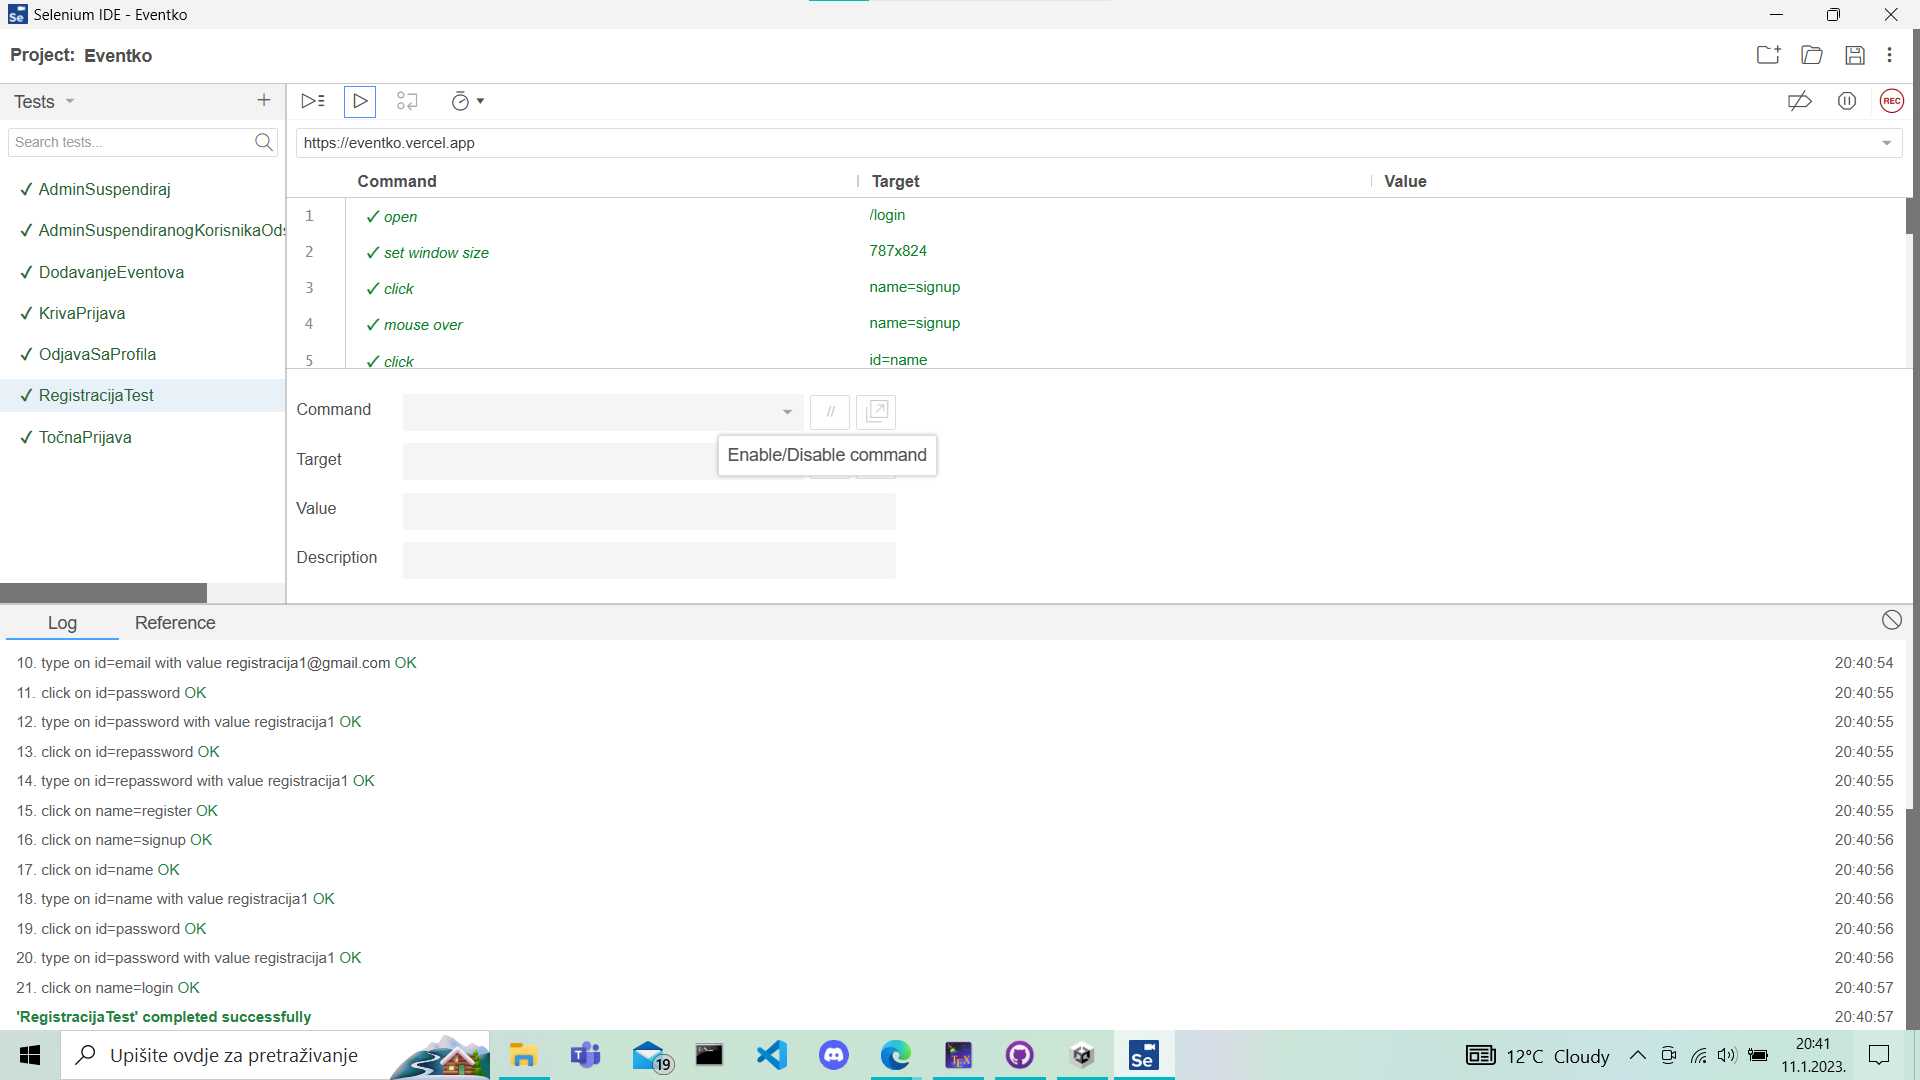
\includegraphics[width=\textwidth]{Slike/RegistracijaTest.png}
		 		\caption{Točna registracija}
		 	\end{figure}
	 	
	 		\indent Za test krive prijave koriste se ulazni podaci "VIDOJE" za korisničko ime i "VIDOJE" za zaporku(za vrijeme prijave ne postoji korisnik sa istim podacima). Pritiskom na gumb prijavi pojavljuje se poruka "Neuspješna prijava" koja se može vidjeti na drugoj slici.
	 		
	 		\begin{figure}[H]
	 			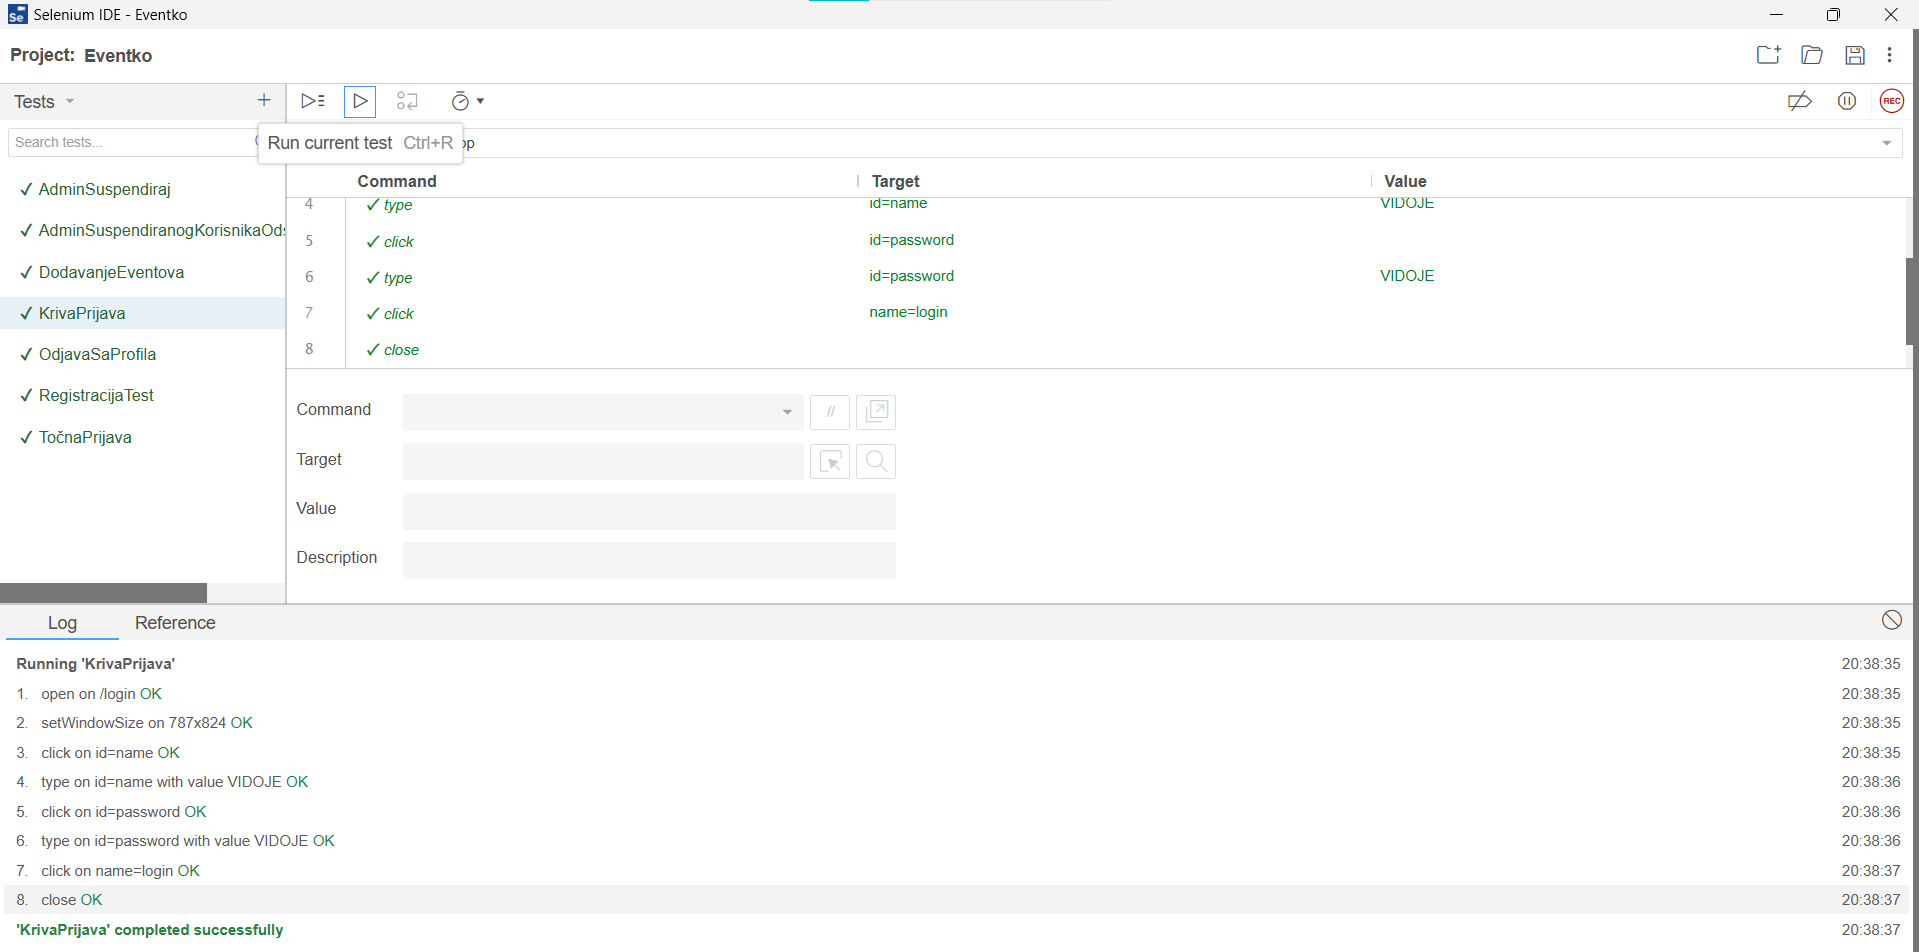
\includegraphics[width=\textwidth]{Slike/KrivaPrijava.png}
	 			\caption{Krivi podaci za prijavu}
	 		\end{figure}
 		
 			\begin{figure}[H]
 				\includegraphics[width=\textwidth]{Slike/Neuspješna prijava.png}
 				\caption{Neuspješna prijava}
 			\end{figure}
 		
 			\indent Za test odjave sa profila koriste se ulazni podaci "admin" za korisničko ime i "1234" za zaporku(postoji korisnik sa upisanim ulaznim podacima). Nakon toga se nalazimo na početnoj stranici te stisnemo tekst "Odjava" u desnom gornjem kutu i vraćeni smo na stranicu za prijavu.
 			
 			\begin{figure}[H]
 				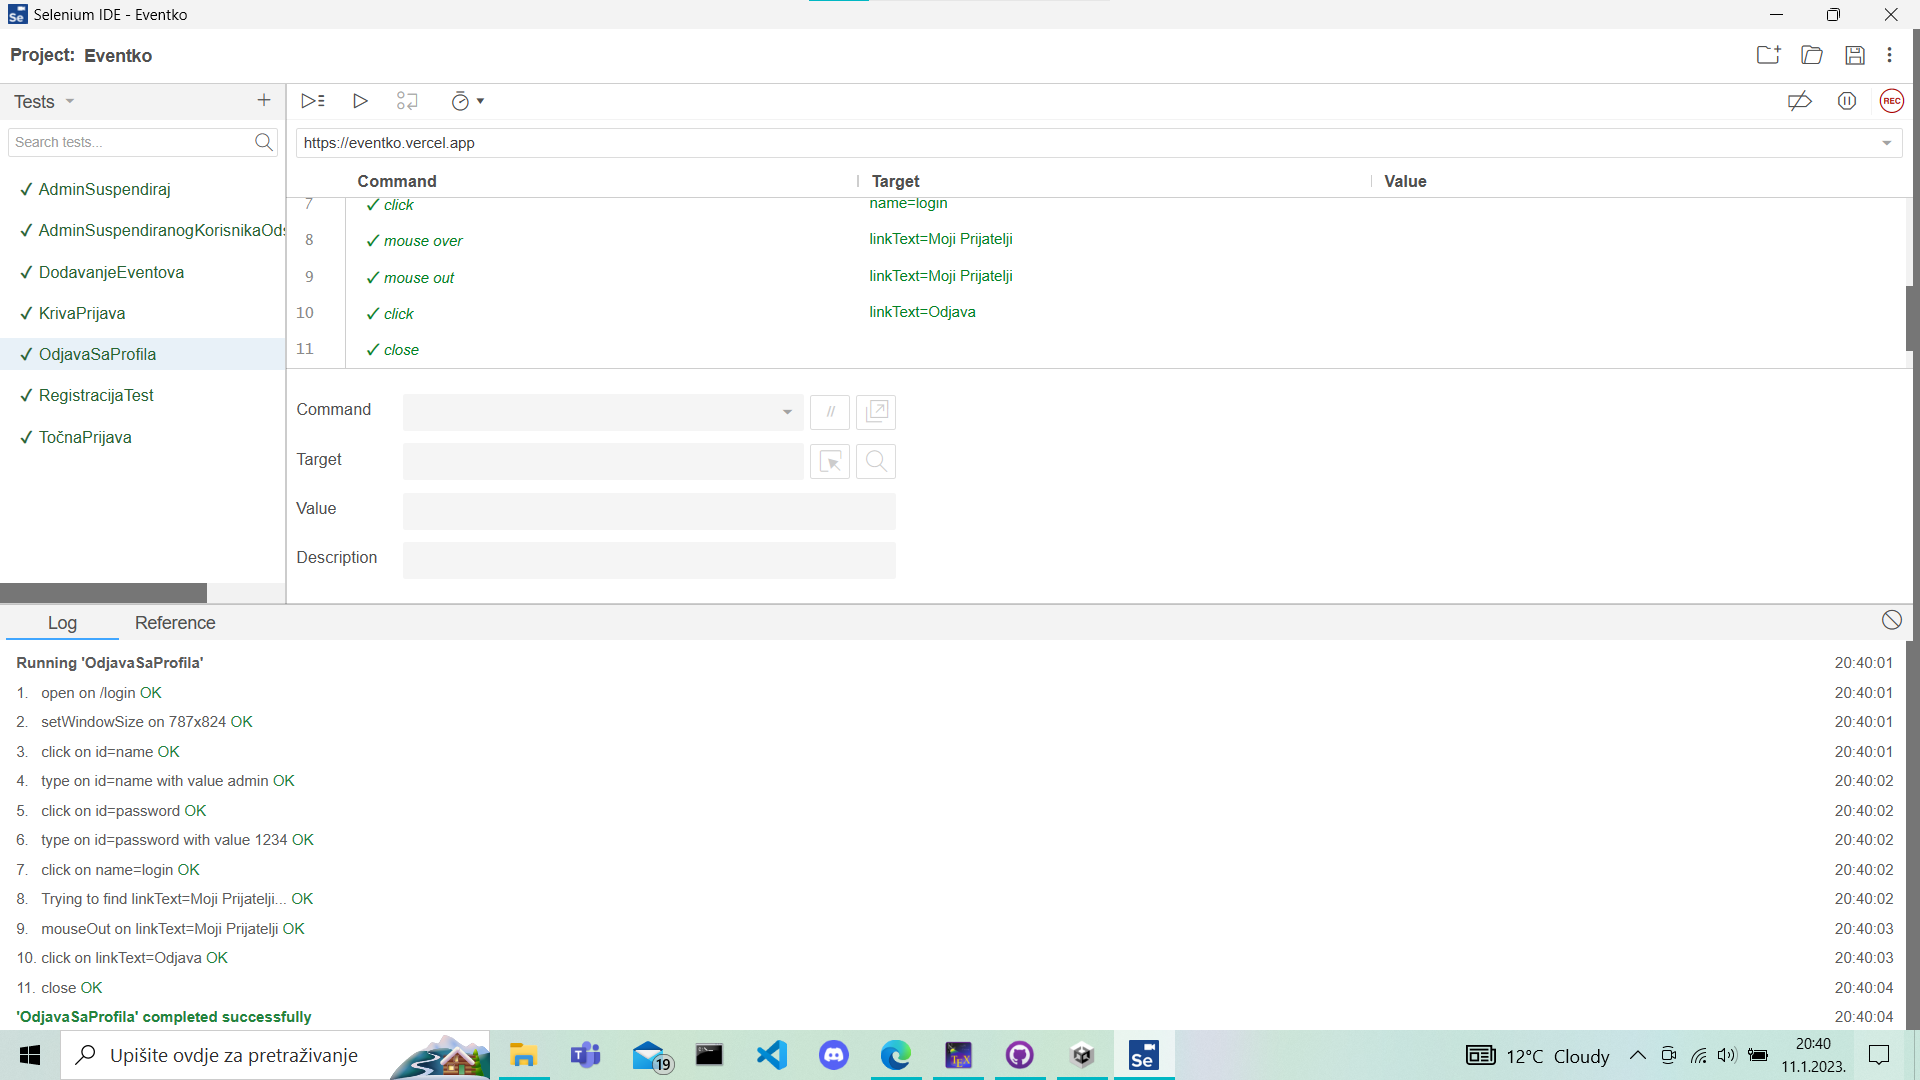
\includegraphics[width=\textwidth]{Slike/OdjavaSaProfila.png}
 				\caption{Odjava sa profila}
 			\end{figure}
 		
 			\indent Za test dodavanja događaja koriste se ulazni podaci "admin" za korisničko ime i "1234" za zaporku(postoji korisnik sa upisanim ulaznim podacima). Nakon toga se nalazimo na početnoj stranici te stisnemo "Dodaj u kalendar" u lijevom gornjem kutu. Nakon toga se otvara prozor za koji se koriste ulazni podaci "Event" za naziv događaja, "Zagreb" za mjesto događaja, "1.2.2023 i 20:21" se odabire za početak događaja i "2.2.2023 i 20:21" se odabire za kraj događaja, te "Javni događaj" se odabire za vrstu događaja, "Kava" se odabire za oznaku događaja i "Ucenje" za opis događaja. Stvoren je novi događaj i vidljiv je u kalendaru kao na drugoj slici.
 			\begin{figure}[H]
 				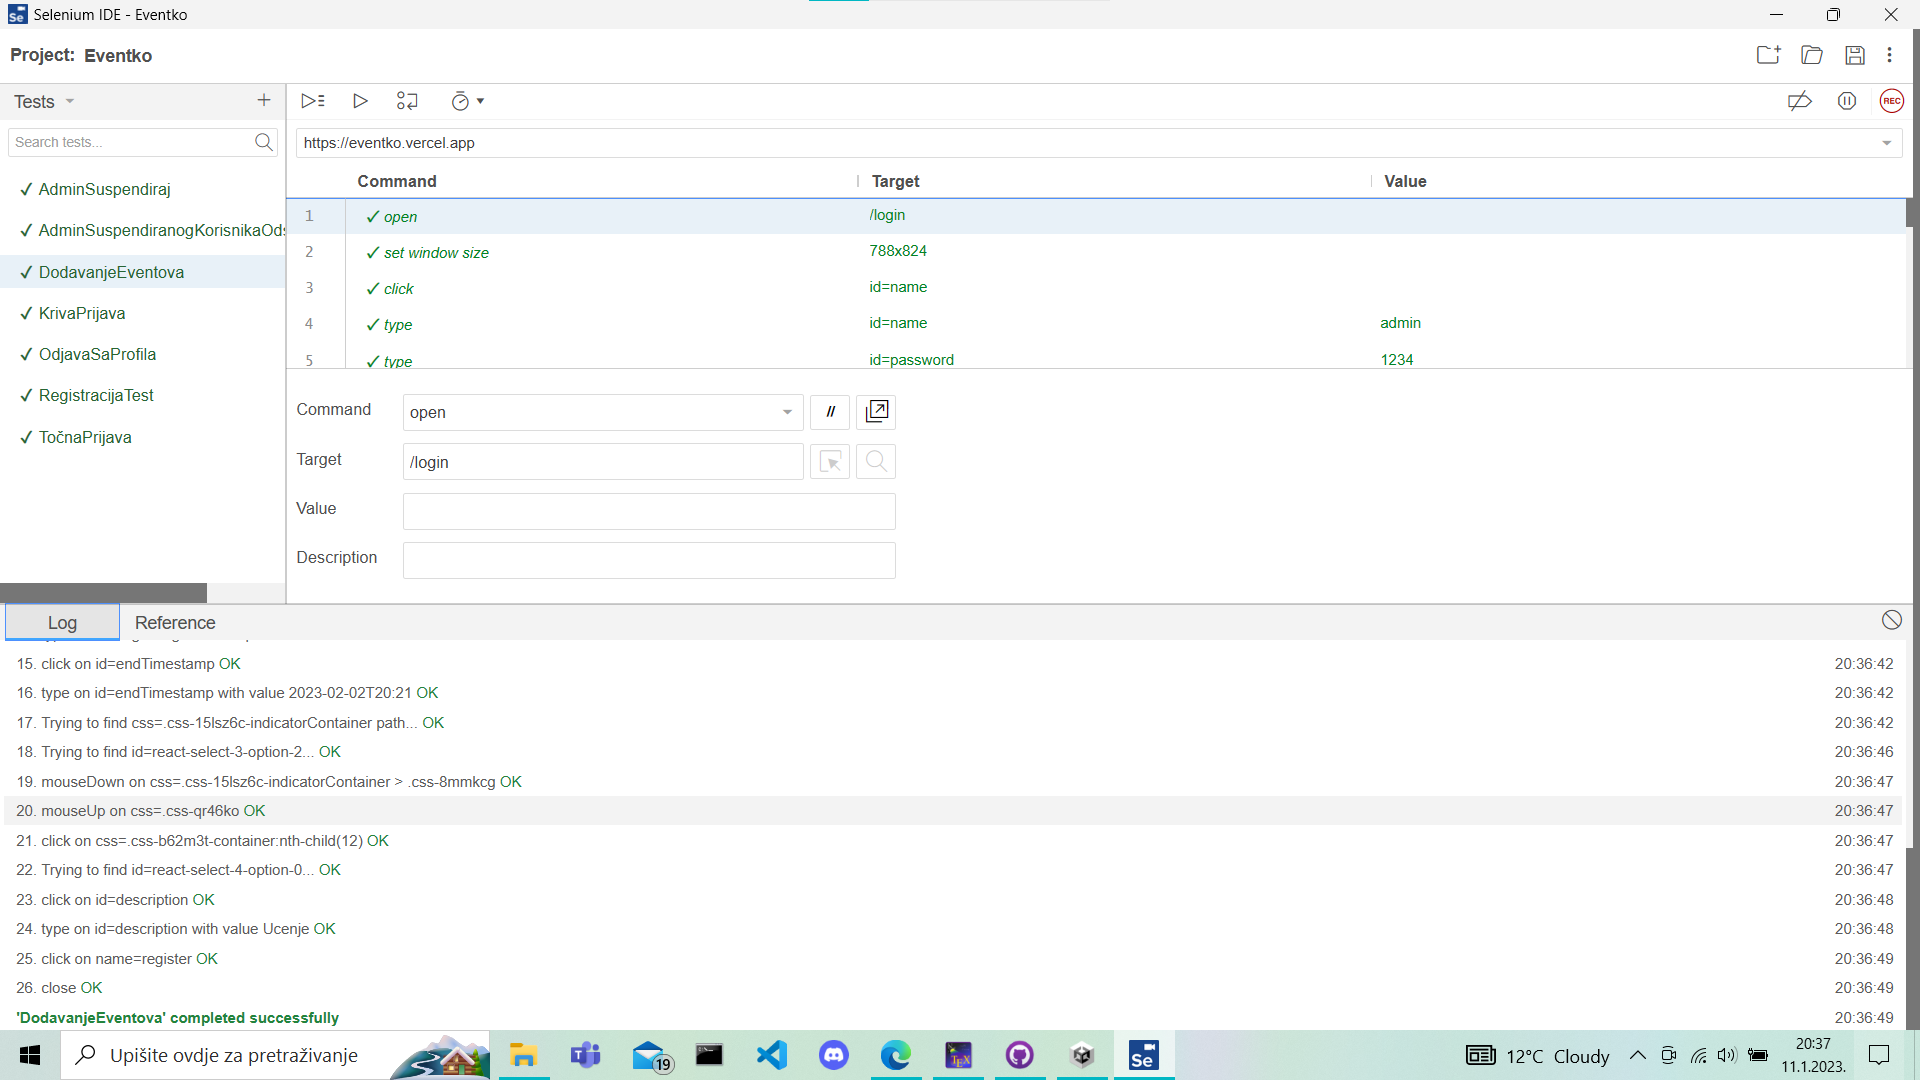
\includegraphics[width=\textwidth]{Slike/DodavanjeEventova.png}
 				\caption{Dodavanje novog događaja}
 			\end{figure}
 		
 			\begin{figure}[H]
 				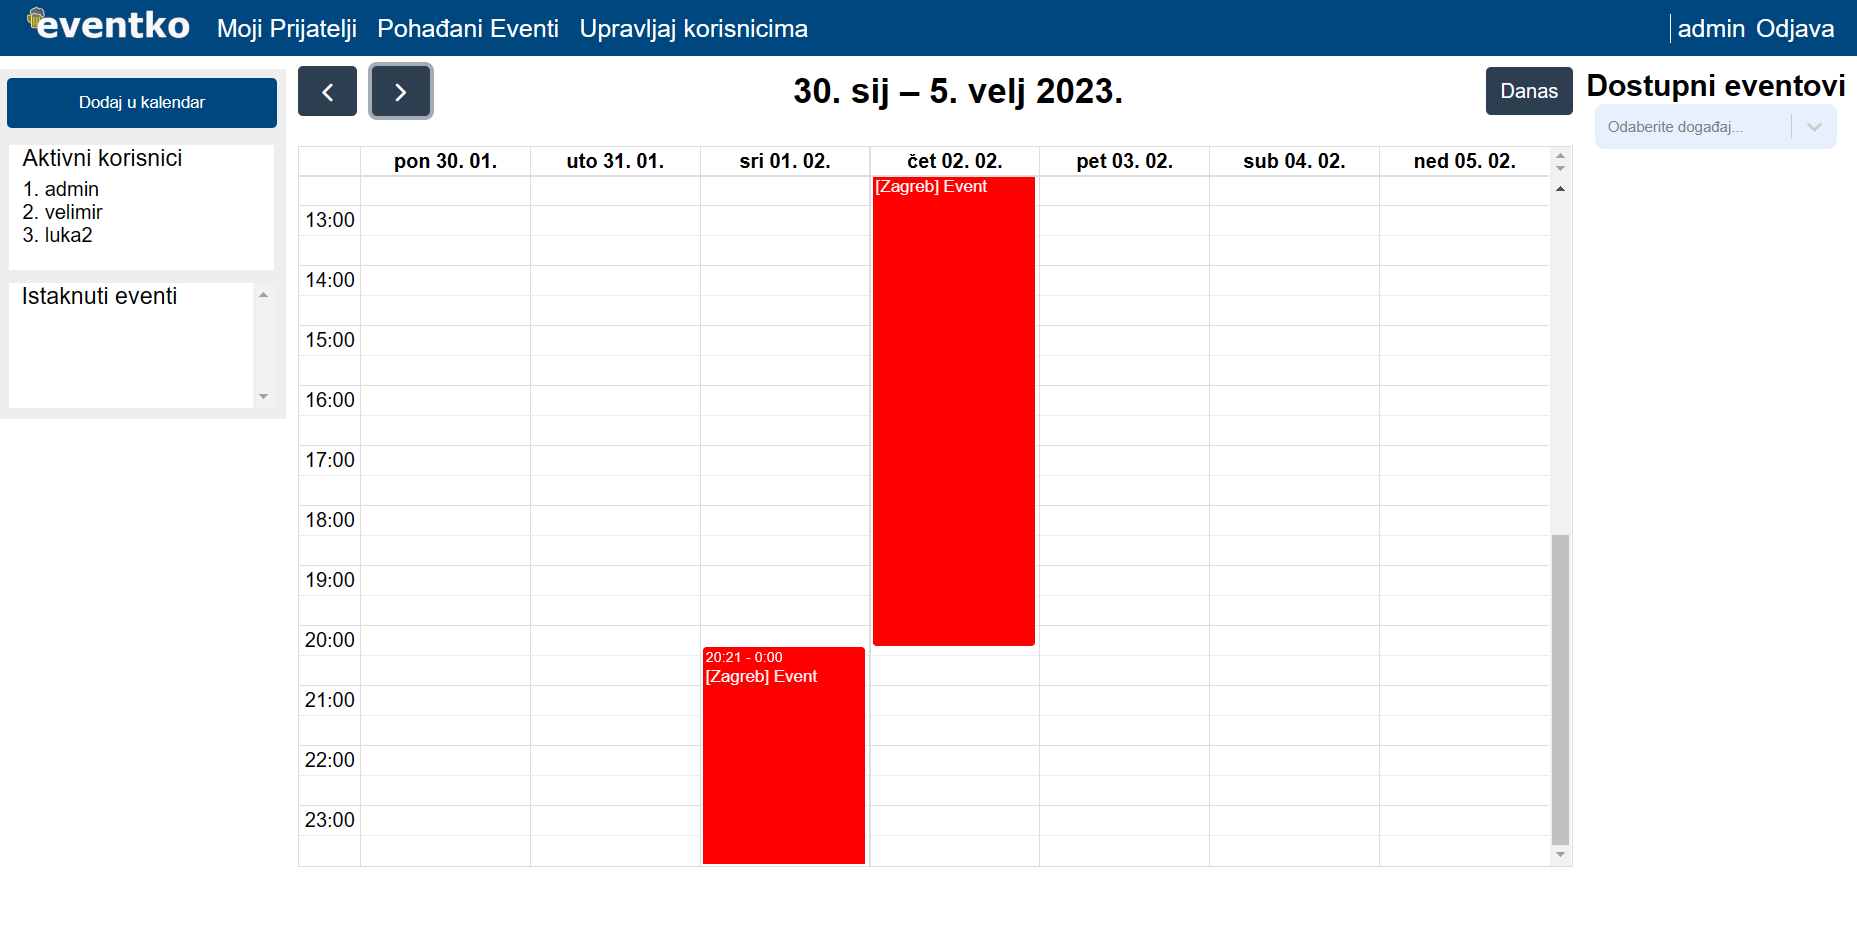
\includegraphics[width=\textwidth]{Slike/Kalendar.png}
 				\caption{Stvoren novi događaj u kalendaru}
 			\end{figure}
 			
 			\indent Za test suspendiranje korisnika koriste se ulazni podaci "admin" za korisničko ime i "1234" za zaporku(postoji korisnik sa upisanim ulaznim podacima te ima i ovlasti admina). Nakon toga se nalazimo na početnoj stranici te stisnemo "Upravljaj korisnicima". Stisnemo gumb suspendiraj i željeni korisnik je suspendiran.
 			
 			\begin{figure}[H]
 				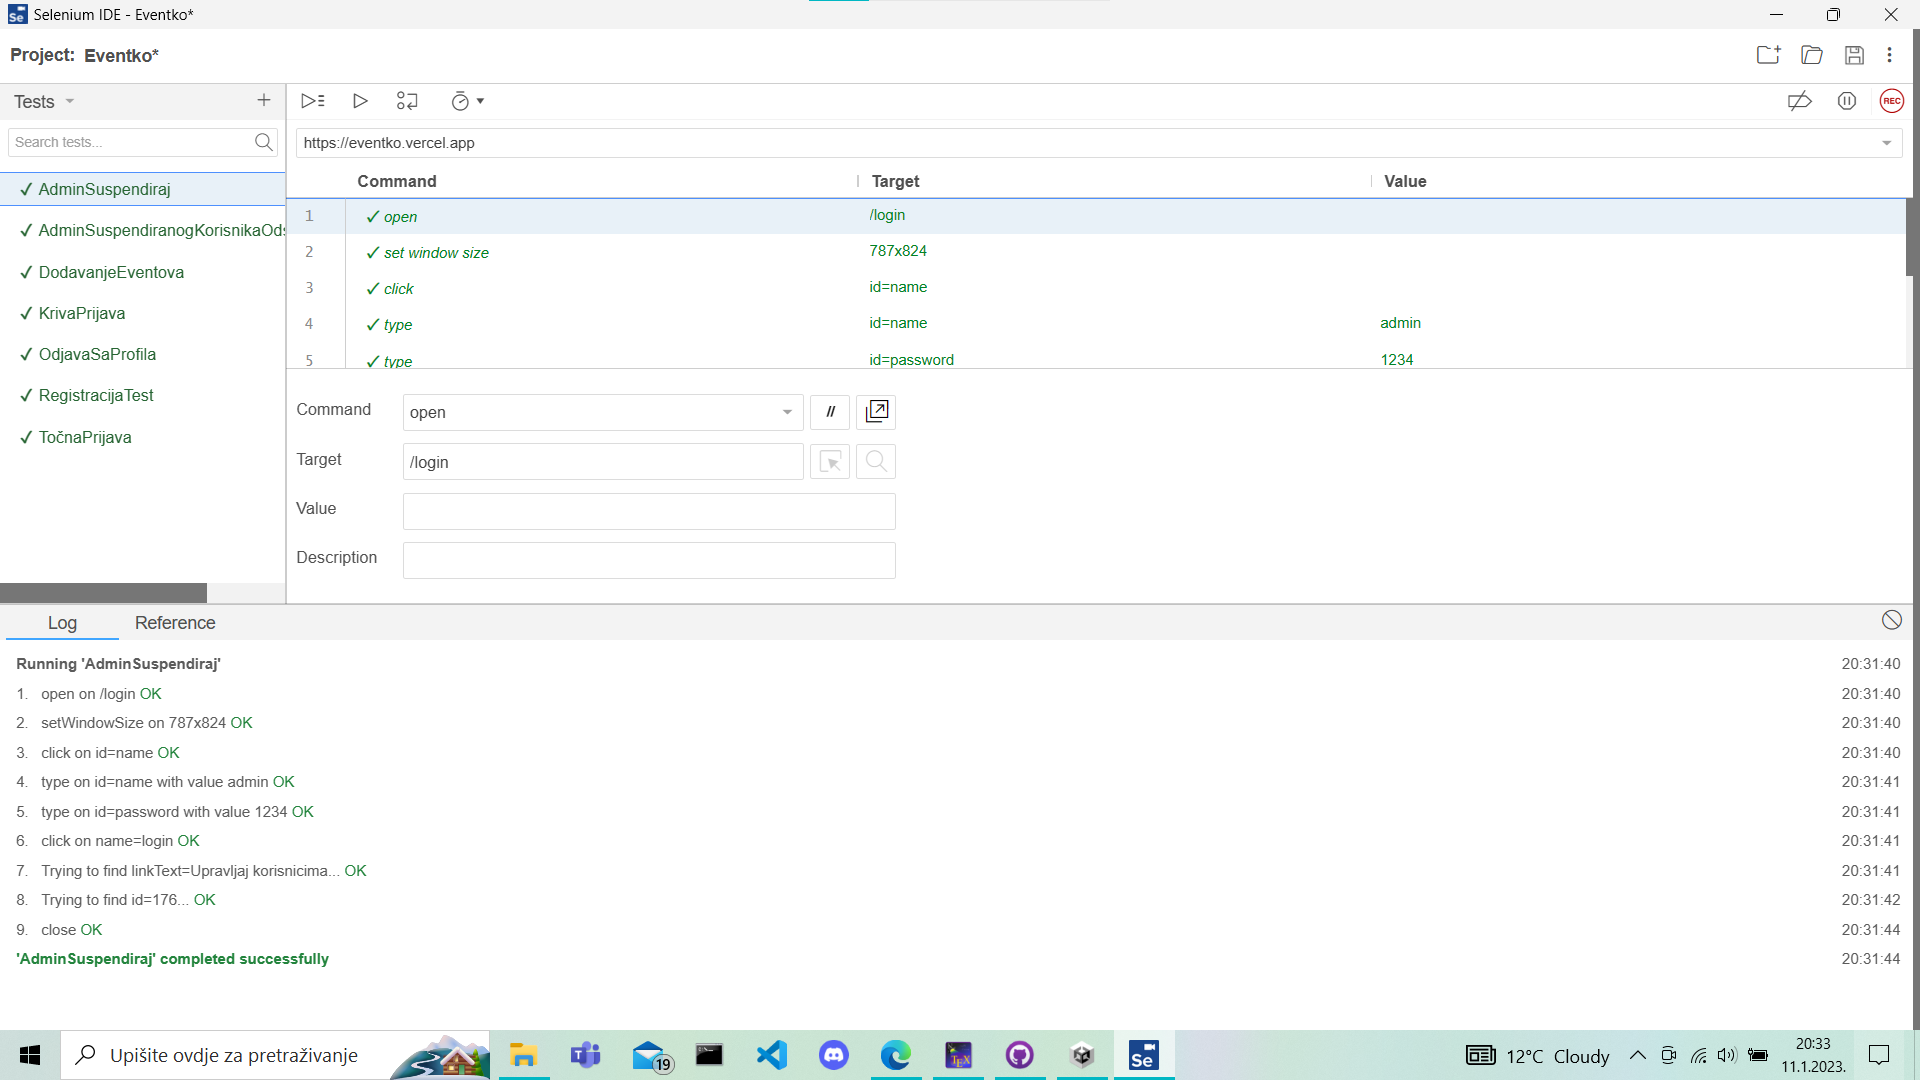
\includegraphics[width=\textwidth]{Slike/AdminSuspendirajSelenium.png}
 				\caption{Admin suspendiranje}
 			\end{figure}
 		
 		
 			\indent Za test odsuspendiranja korisnika koriste se ulazni podaci "admin" za korisničko ime i "1234" za zaporku(postoji korisnik sa upisanim ulaznim podacima te ima i ovlasti admina). Nakon toga se nalazimo na početnoj stranici te stisnemo "Upravljaj korisnicima". Stisnemo gumb odsuspendiraj i željeni korisnik je odsuspendiran.
 			
 			\begin{figure}[H]
 				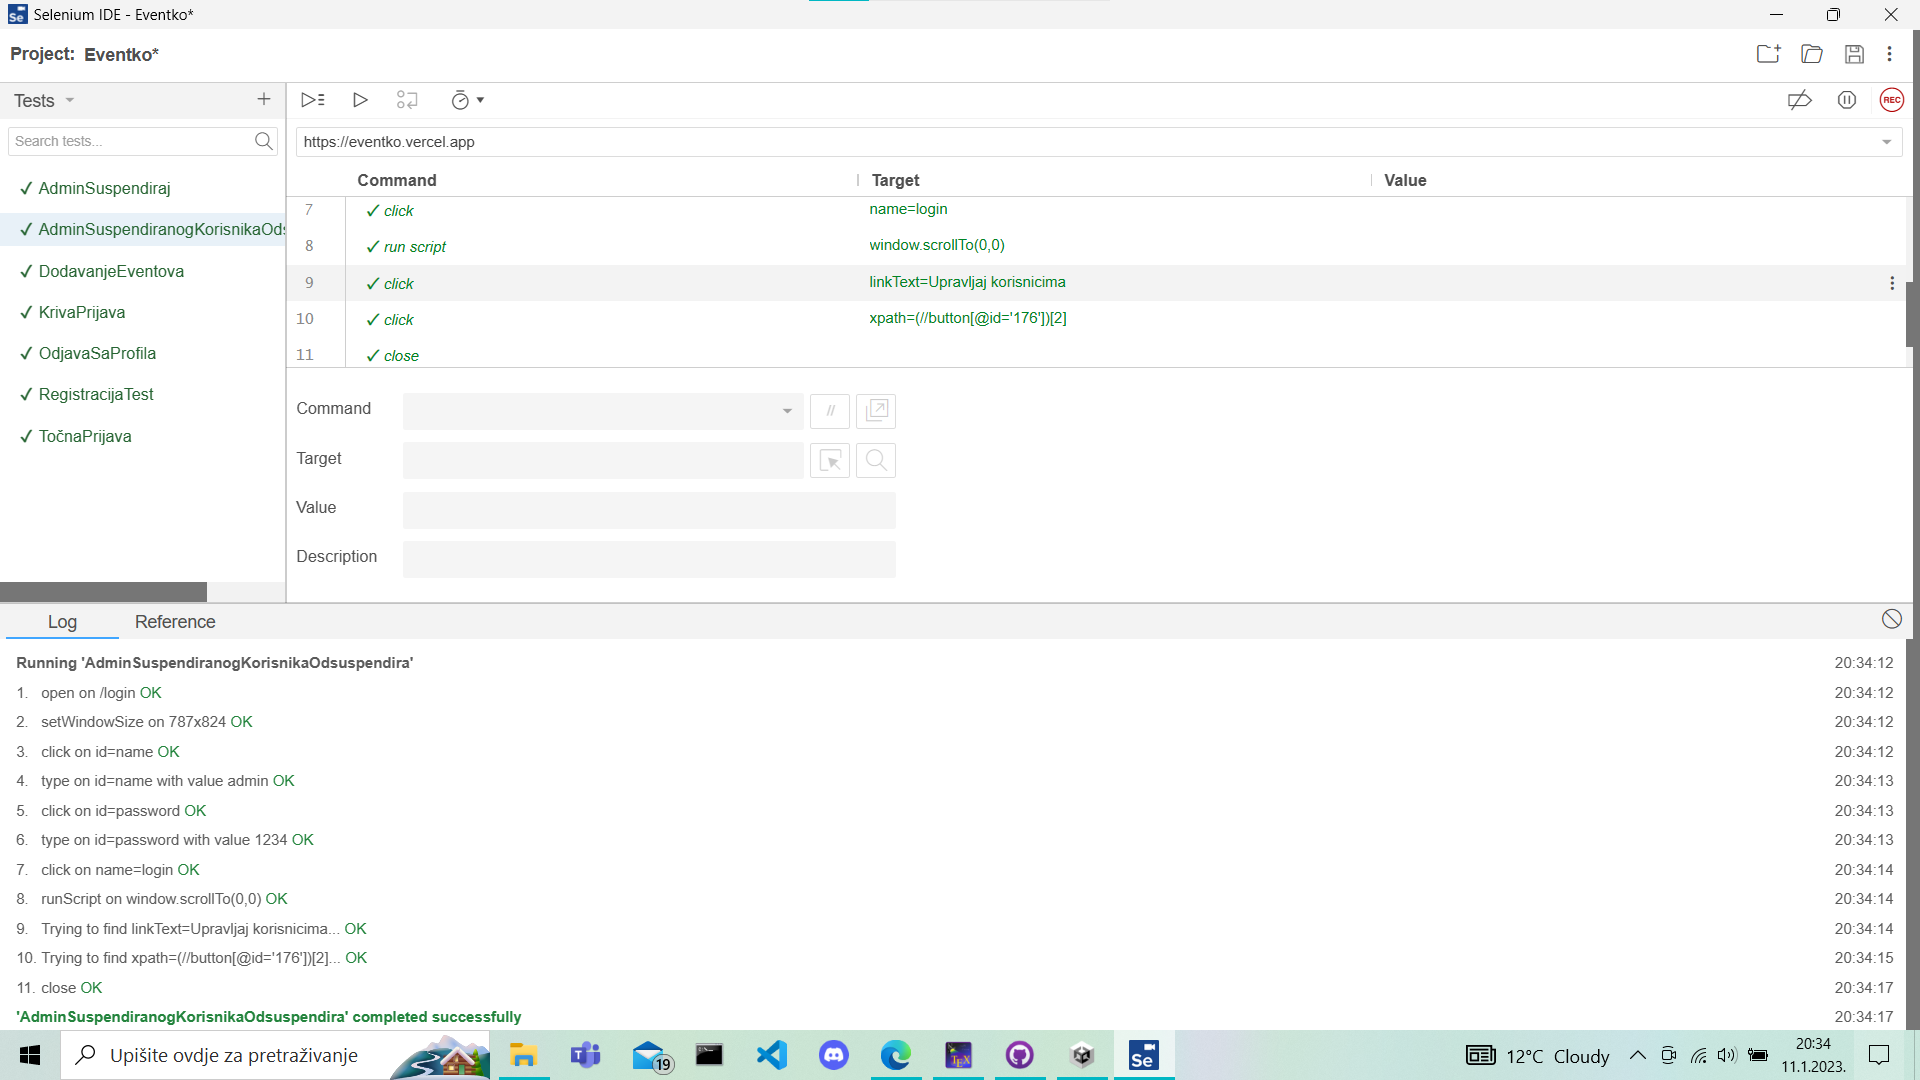
\includegraphics[width=\textwidth]{Slike/AdminSuspendiranogKorisnikaOdsuspendiraj.png}
 				\caption{Admin odsuspendiranje}
 			\end{figure}
 		
		 	
			
			\eject 
		
			
		\section{Dijagram razmještaja}
			
			 \indent Dijagram razmještaja opisuje topologiju sklopovlja i programsku potporu koja se koristi u implementaciji sustava u njegovom radnom okruženju. Na poslužiteljskom računalu se nalaze web poslužitelj na renderu i poslužitelj baze podataka na vercelu. Sustav je baziran na arhitekturi "klijent - poslužitelj", a komunikacija između računala korisnika (običan korisnik, premium korisnik, pregledavač, moderator, administrator) i poslužitelja odvija se preko HTTP veze.
			 
			 \begin{figure}[H]
			 	\includegraphics[width=\textwidth]{Dijagrami/Dijagram Razmještaja.png}
			 	\caption{Dijagram razmještaja}
			 \end{figure}
			
			\eject 
		
		\section{Upute za puštanje u pogon}
		
			\indent Puštanje web aplikacije u pogon sastoji se od tri segmenta:
			\begin{itemize}
				\item Stvaranje baze podataka
				\item Puštanje backenda u pogon
				\item Puštanje frontenda u pogon
			\end{itemize}
		
			\noindent \textbf{Stvaranje baze podataka}\\
			
			\indent Baza podataka besplatno je spremljena na web-oblaku render.com. Ona se postavlja i osposobljava sljedećim koracima:
			
			\begin{packed_enum}
				\item Stvaranje nove baze
				\begin{itemize}
					\item Za početak je potrebno (nakon registracije na render.com) odabrati opciju \textit{New} te na padajućem izborniku \textit{PostgreSQL}
					\item Pojavljuje se izbornik koji ispunjavamo kao na slici ispod
					\item Biramo \textit{Create Database}
				\end{itemize}
				\begin{figure}[H]
					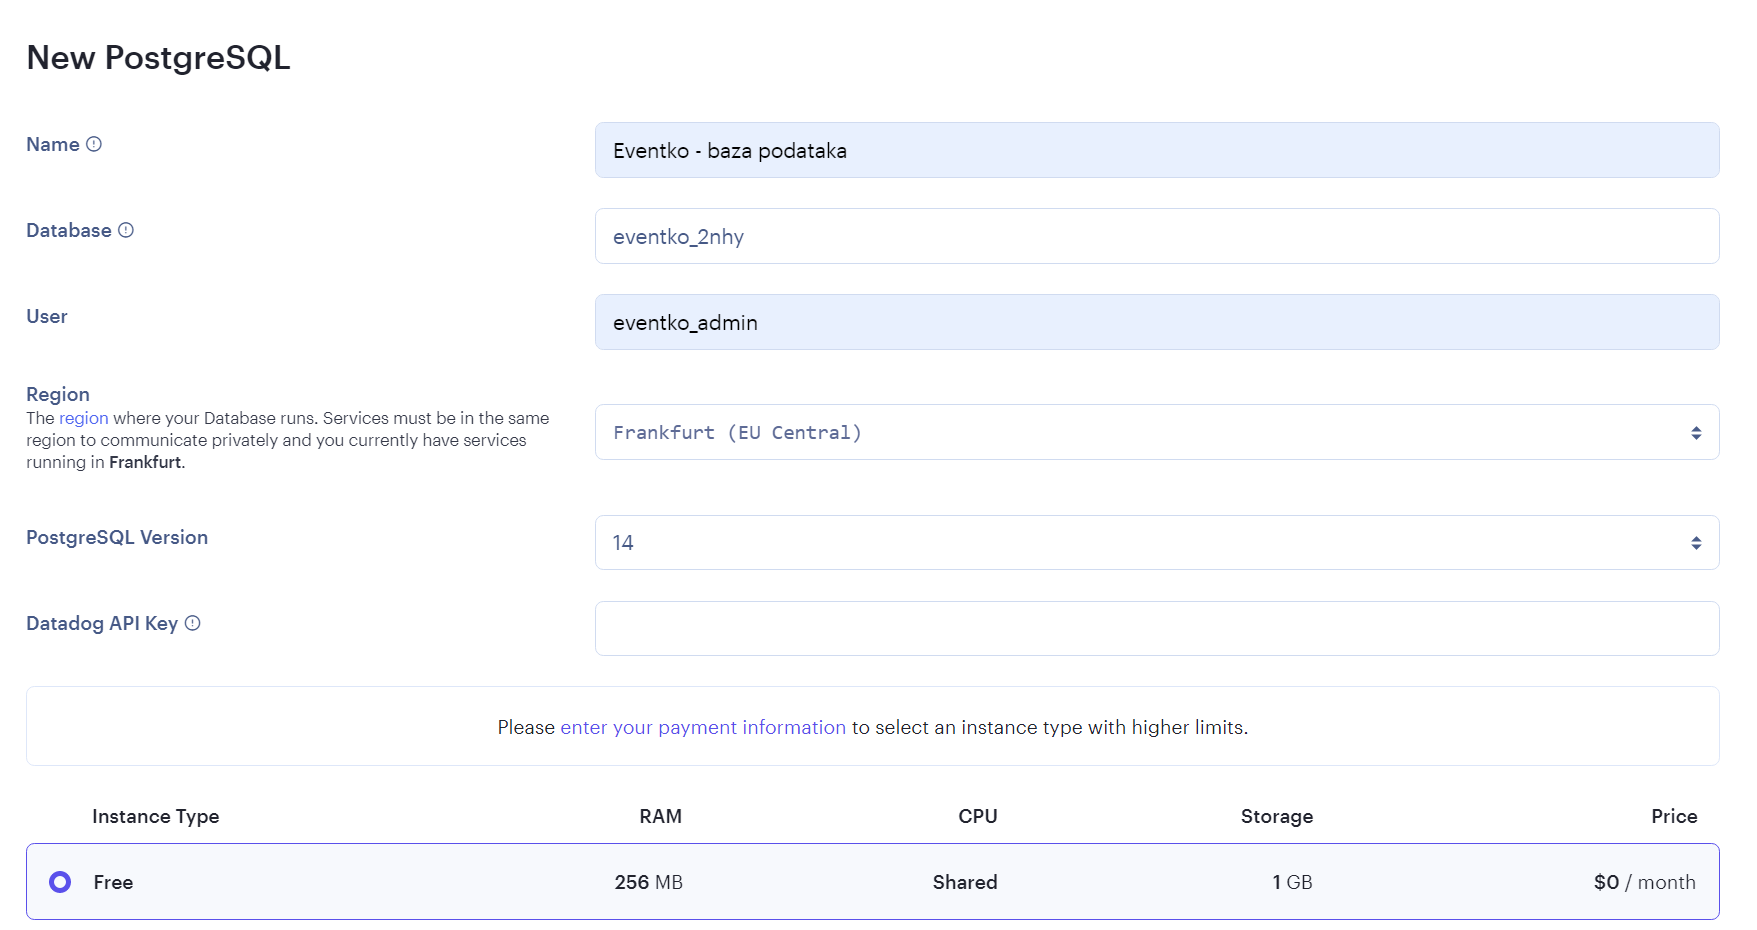
\includegraphics[width=\textwidth]{Opis deploymenta/Slika1.png}
					\caption{Stvaranje nove PostgreSQL baze}
				\end{figure}
				\eject
			
				\item Dohvat podataka za spajanje
				\begin{itemize}
					\item Redom biramo \textit{Dashboard} -> \textit{Eventko - baza podataka} -> \textit{Info}
					\item Skrolamo do izbora \textit{Connections} gdje vidimo informacije potrebne za spajanje na bazu (slika ispod).
				\end{itemize}
				\begin{figure}[H]
					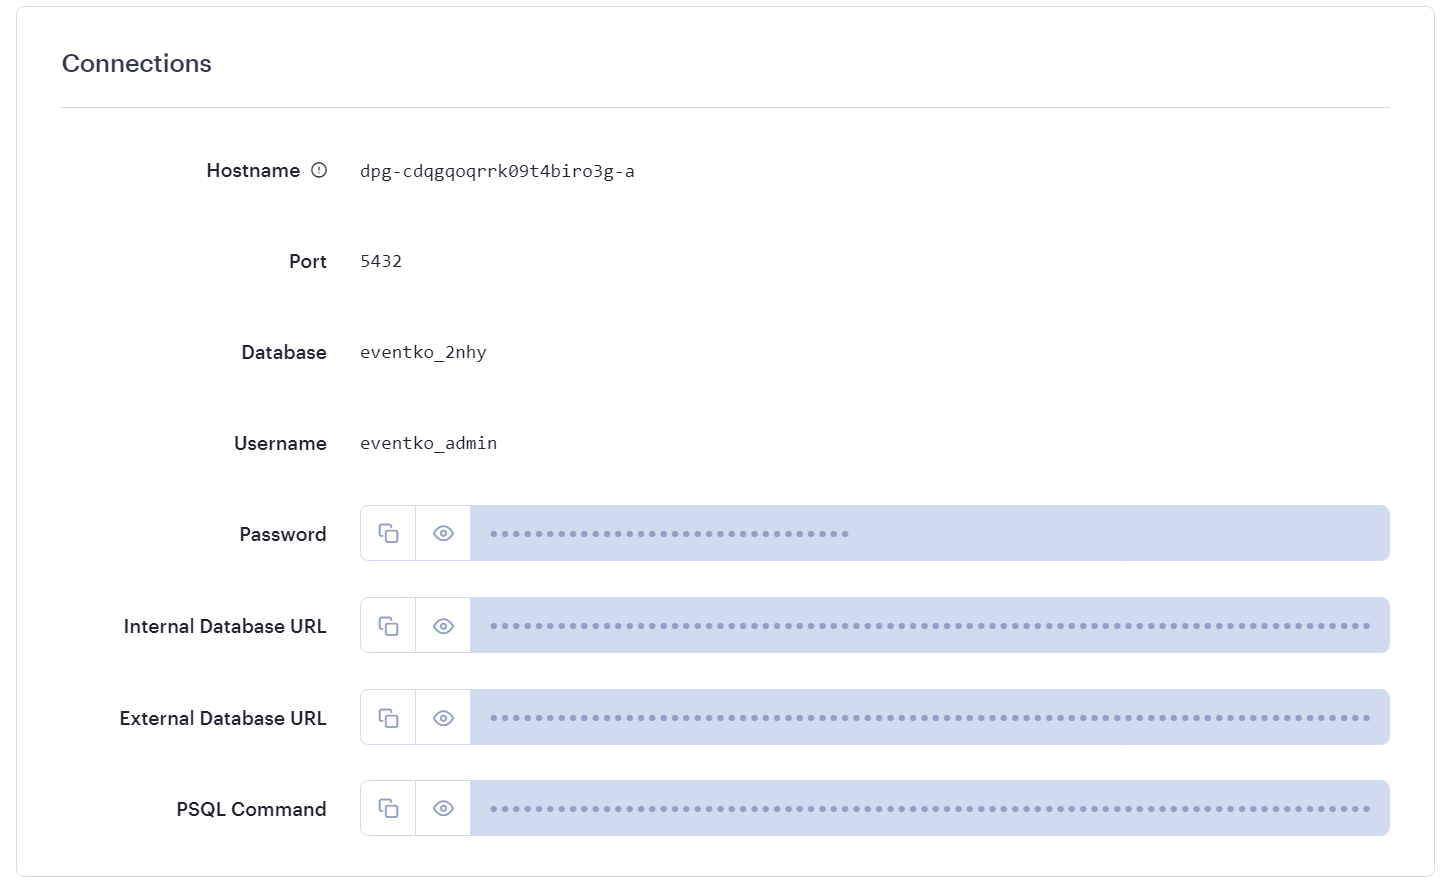
\includegraphics[width=\textwidth]{Opis deploymenta/Slika2.png}
					\caption{Dohvat podataka za spajanje baze}
				\end{figure}
			
				\item Spajanje putem pgAdmina
				\begin{itemize}
					\item Izabiremo \textit{Object} -> \textit{Create} -> \textit{Server}
					\item Na kartici \textit{General} unosimo ime servera kojeg otvaramo u pgAdminu
					\item Na kartici \textit{Connection} unosimo podatke kao na slici i spremamo ih sa \textit{Save}
				\end{itemize}
				\begin{figure}[H]
					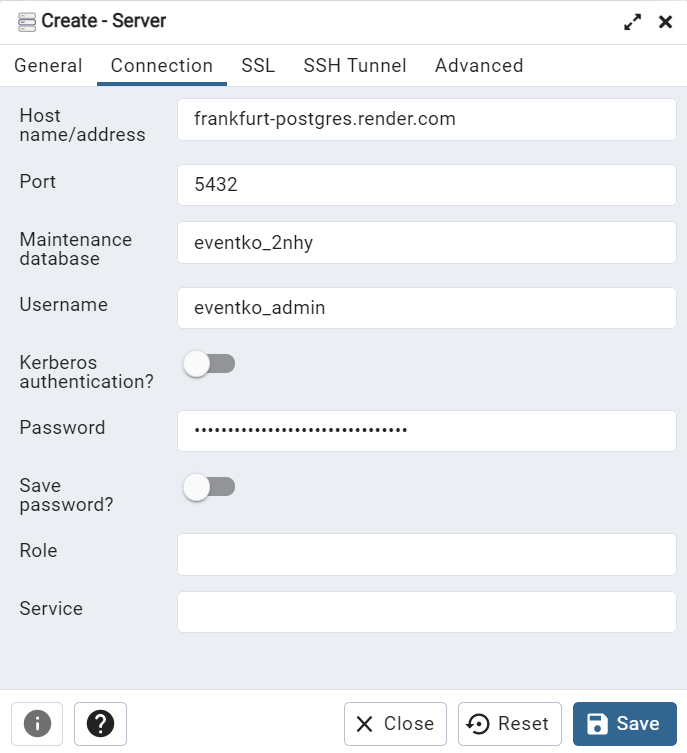
\includegraphics[width=\textwidth]{Opis deploymenta/Slika3.png}
					\caption{Unos podataka za spajanje baze}
				\end{figure}
			
				\item Spajanje iz backenda
				\begin{itemize}
					\item U src/main/resources/application.properties upisujemo naredbe sa slike
				\end{itemize}
				\begin{figure}[H]
					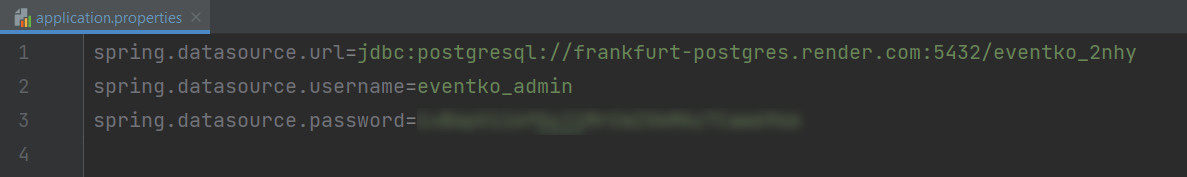
\includegraphics[width=\textwidth]{Opis deploymenta/Slika4.png}
					\caption{Spajanje baze iz backenda}
				\end{figure}
			\end{packed_enum}
			\eject
			
			\noindent \textbf{Puštanje backenda u pogon}\\
			
			\indent Backend dio projekta također koristi render.com za puštanje u pogon. Preduvjeti za to su:		\begin{itemize}
				\item Dodavanje Dockerfilea prikazanog na slici ispod
				\item Povezivanje s GitLabom na renderu
			\end{itemize}
			\begin{figure}[H]
				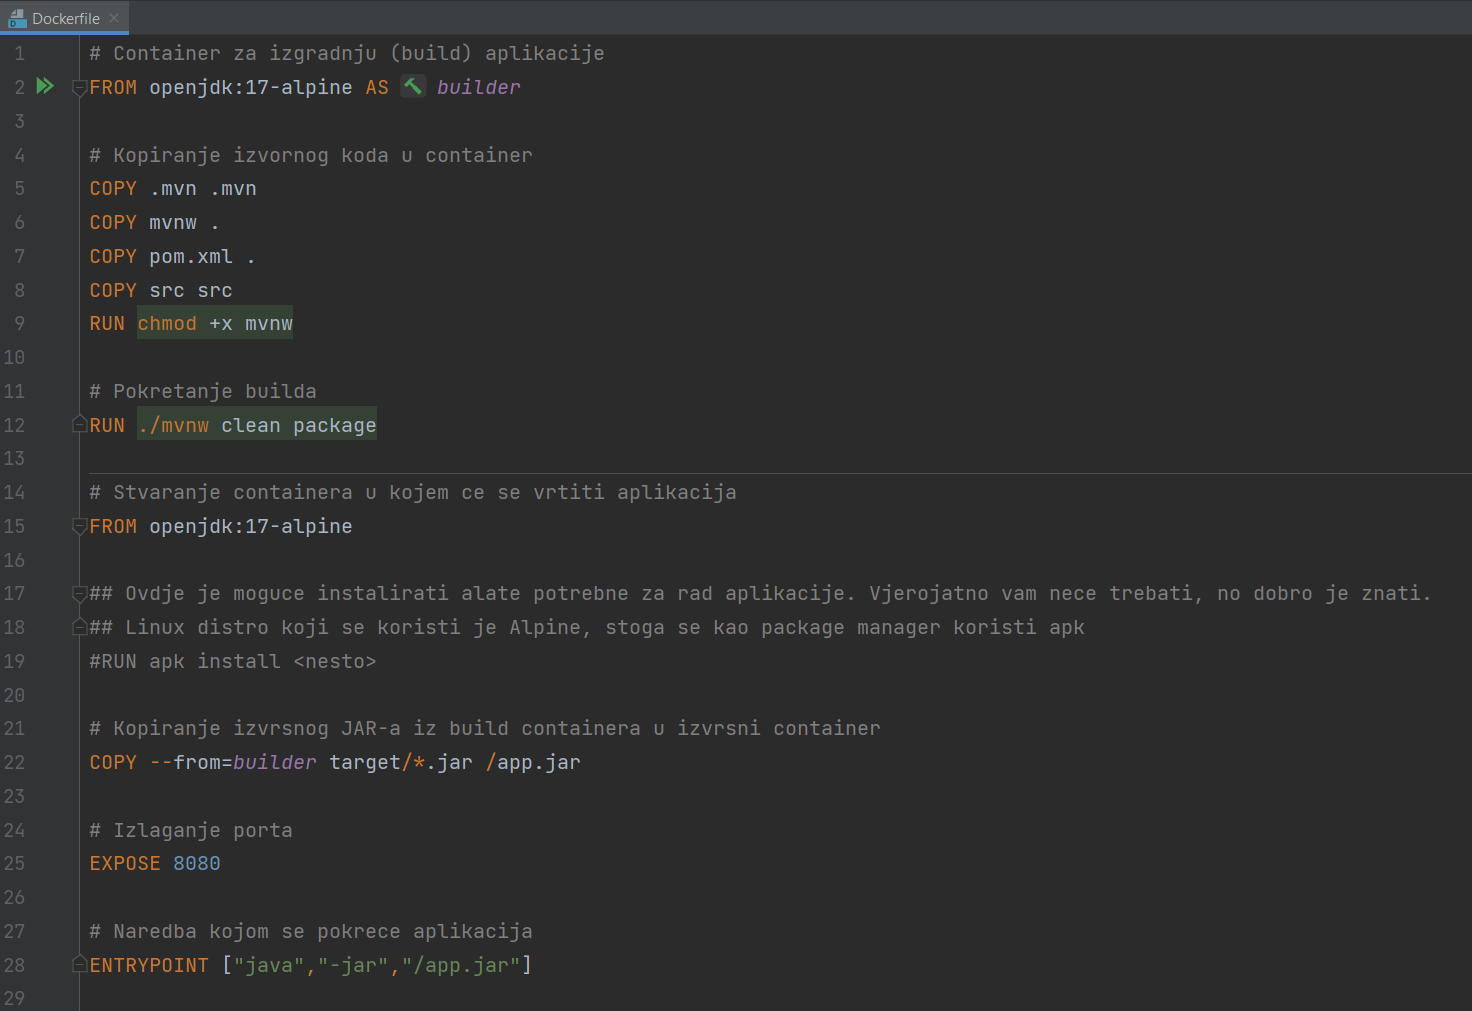
\includegraphics[width=\textwidth]{Opis deploymenta/Slika5.png}
				\caption{Potrebni Dockerfile}
			\end{figure}
		
			\indent Stvaranje backenda postižemo na sljedeći način:
			\begin{itemize}
				\item Odabiremo na render.com \textit{New} -> \textit{Web Service}
				\item Odabiremo željeni GitLab repozitorij
				\item Dalje unosimo podatke kao na slici ispod i potvrđujemo s \textit{Create Web Service}
			\end{itemize}
			\begin{figure}[H]
				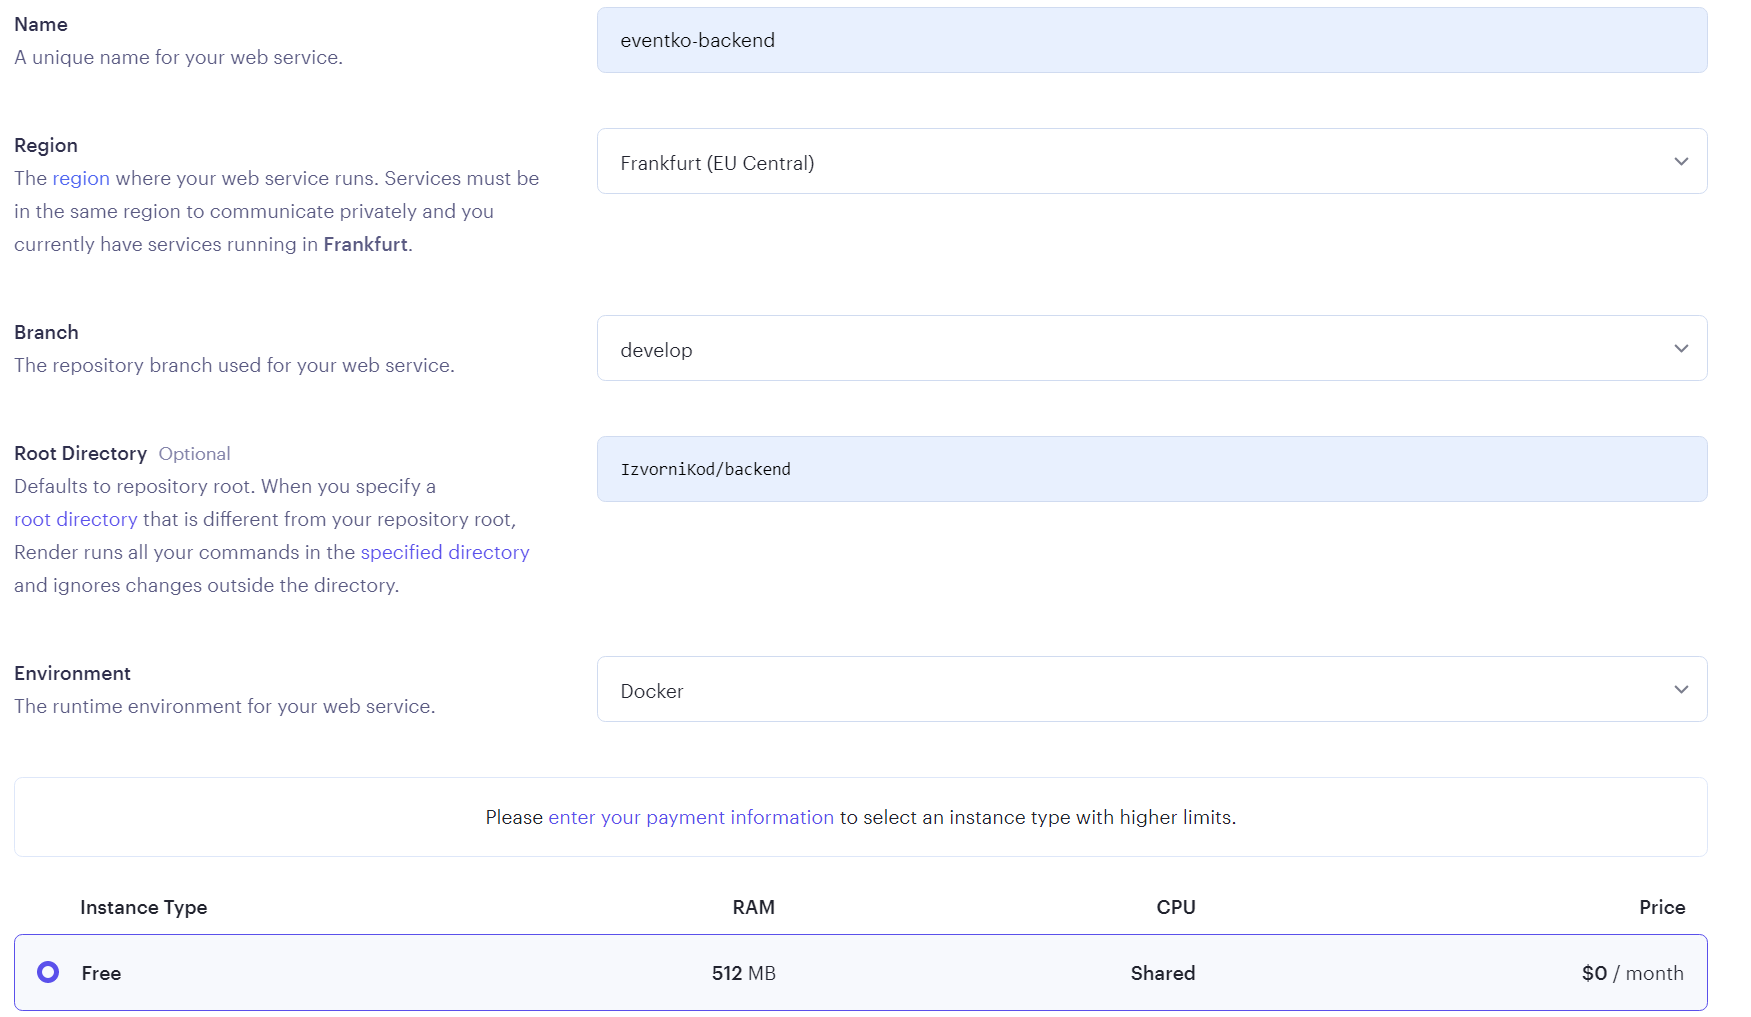
\includegraphics[width=\textwidth]{Opis deploymenta/Slika6.png}
				\caption{Stvaranje novog web servisa}
			\end{figure}
		
			\noindent \textbf{Puštanje frontenda u pogon}\\
			
			\indent Frontend dio projekta puštamo u pogon servisom vercel.com. Preduvjeti za to su:
			\begin{itemize}
				\item Dodavanje vercel.json datoteke u projekt (slika ispod) radi mapiranja putanja prema backendu
				\item Povezivanje s GitLabom i stvaranje grupe na vercelu
			\end{itemize}
		
			\begin{figure}[H]
				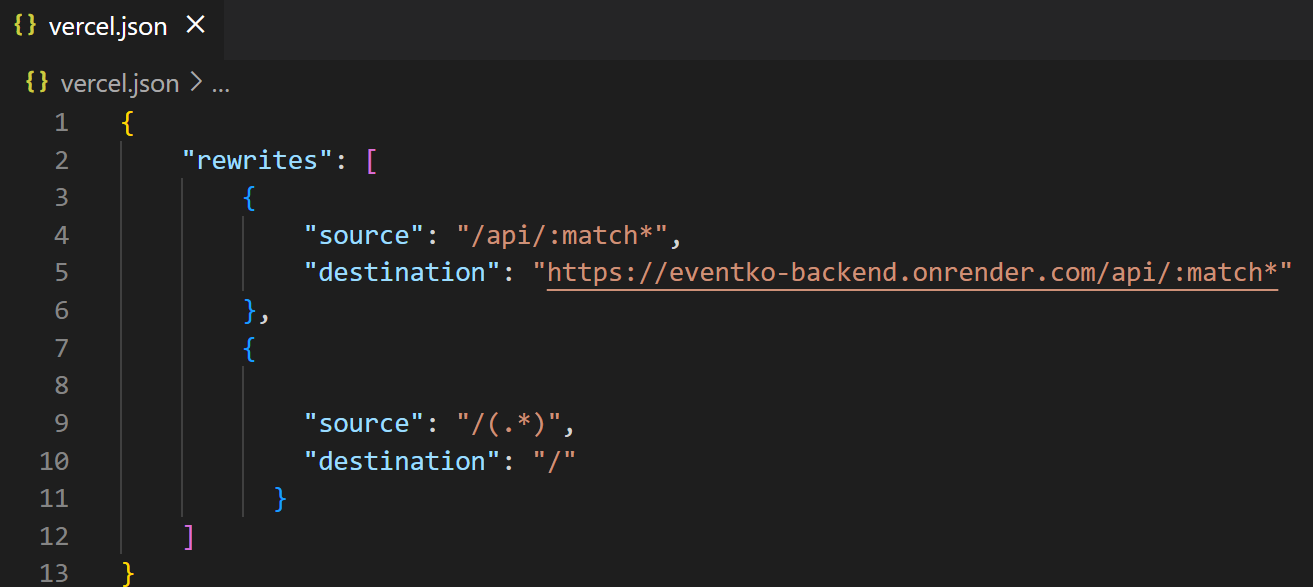
\includegraphics[width=\textwidth]{Opis deploymenta/Slika7.png}
				\caption{Potrebna vercel.json datoteka}
			\end{figure}
			\eject
			
			\indent Za puštanje frontenda u pogon provode se sljedeći koraci:
			\begin{packed_enum}
				\item Stvaranje
				\begin{itemize}
					\item Odabiremo grupu \textit{Vidoje} od ponuđenih iz našeg GitLab računa
					\item Biramo redom \textit{Add new} pa \textit{Import git repository}, pri čemu biramo repozitorij Eventko
					\item Odabiremo \textit{Configure Project}, ispunjavamo polja kao na slici ispod i završavamo s \textit{Deploy}
				\end{itemize}
				\begin{figure}[H]
					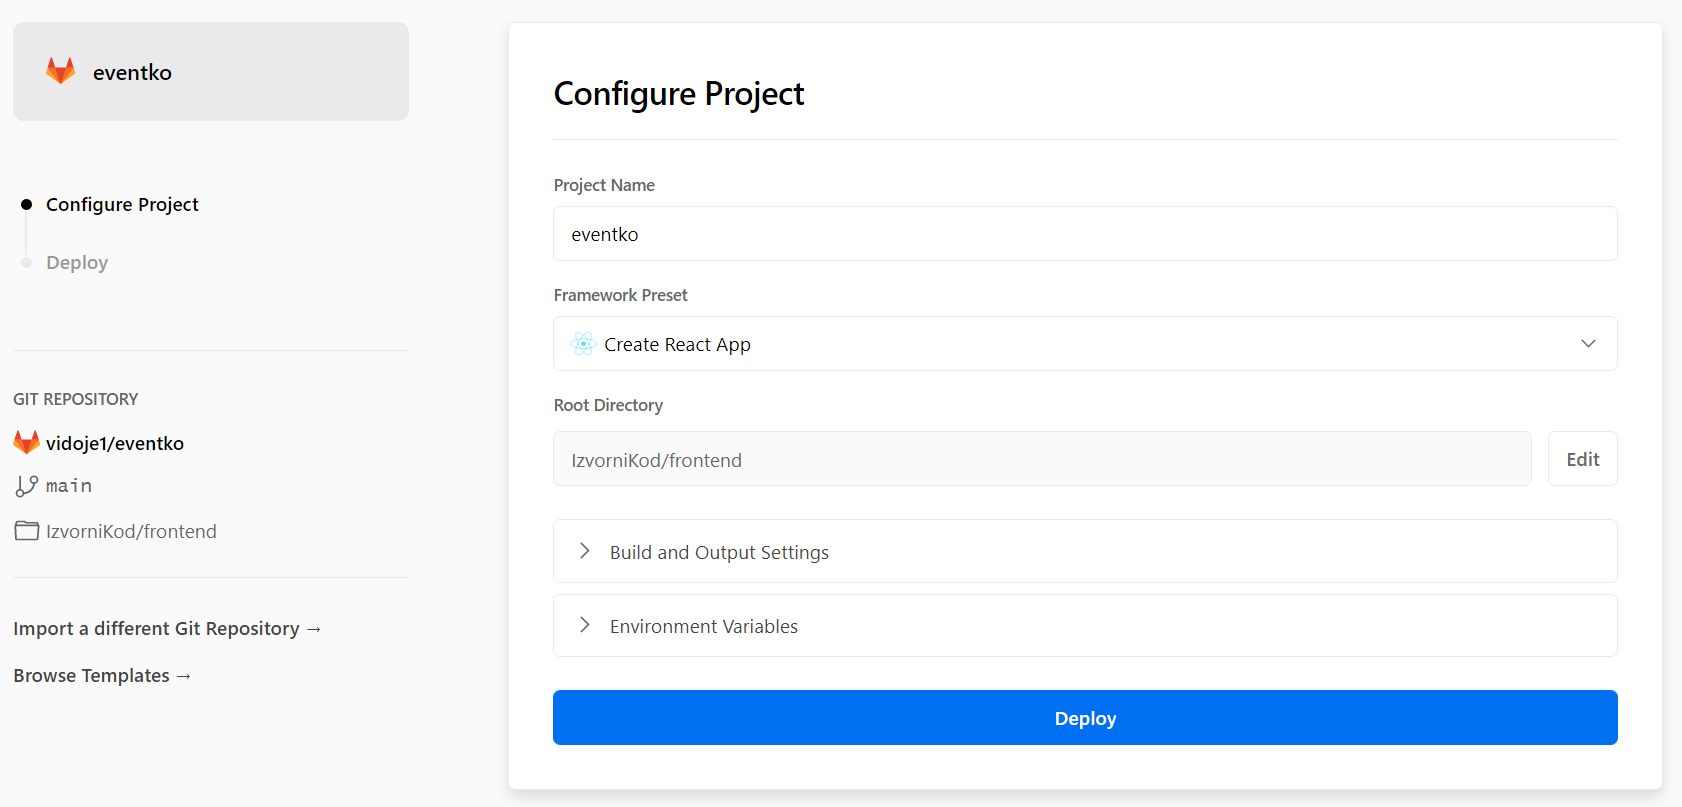
\includegraphics[width=\textwidth]{Opis deploymenta/Slika8.png}
					\caption{Stvaranje React aplikacije i puštanje u pogon}
				\end{figure}
				
				\item Promjena grane
				\begin{itemize}
					\item Biramo redom \textit{Overview} -> \textit{Eventko} -> \textit{Settings} -> \textit{Git}
					\item Mijenjamo granu iz \textit{main} u \textit{develop} kao na slici ispod te spremamo sa \textit{Save}
				\end{itemize}
				\begin{figure}[H]
					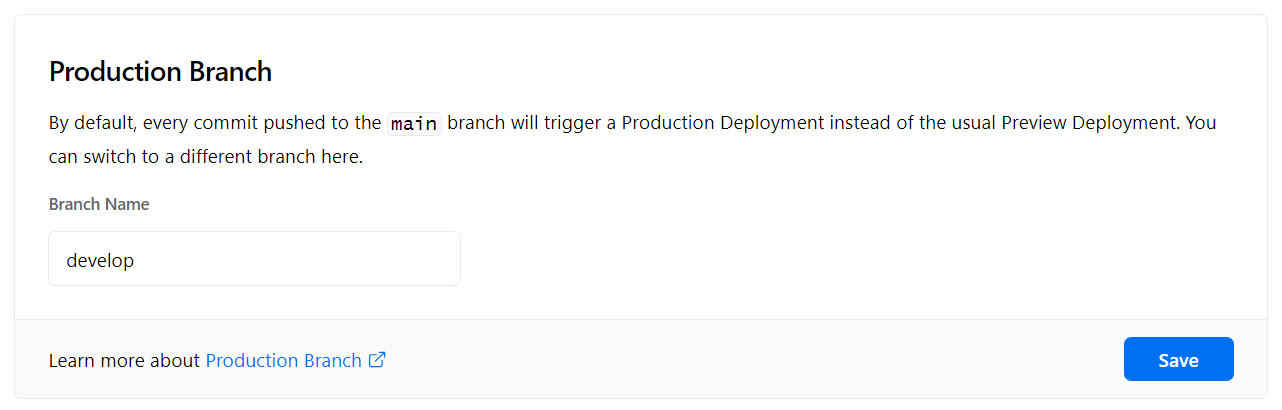
\includegraphics[width=\textwidth]{Opis deploymenta/Slika9.png}
					\caption{Promjena razvojne grane}
				\end{figure}
				\eject
				
				\item Izmjena dodijeljene domene web-stranice (opcionalno)
				\begin{itemize}
					\item Biramo redom \textit{Overview} -> \textit{Eventko} -> \textit{Settings} -> \textit{Domains}
					\item Unosimo novu željenu domenu kao na slici ispod i spremamo sa \textit{Save}
				\end{itemize}
				\begin{figure}[H]
					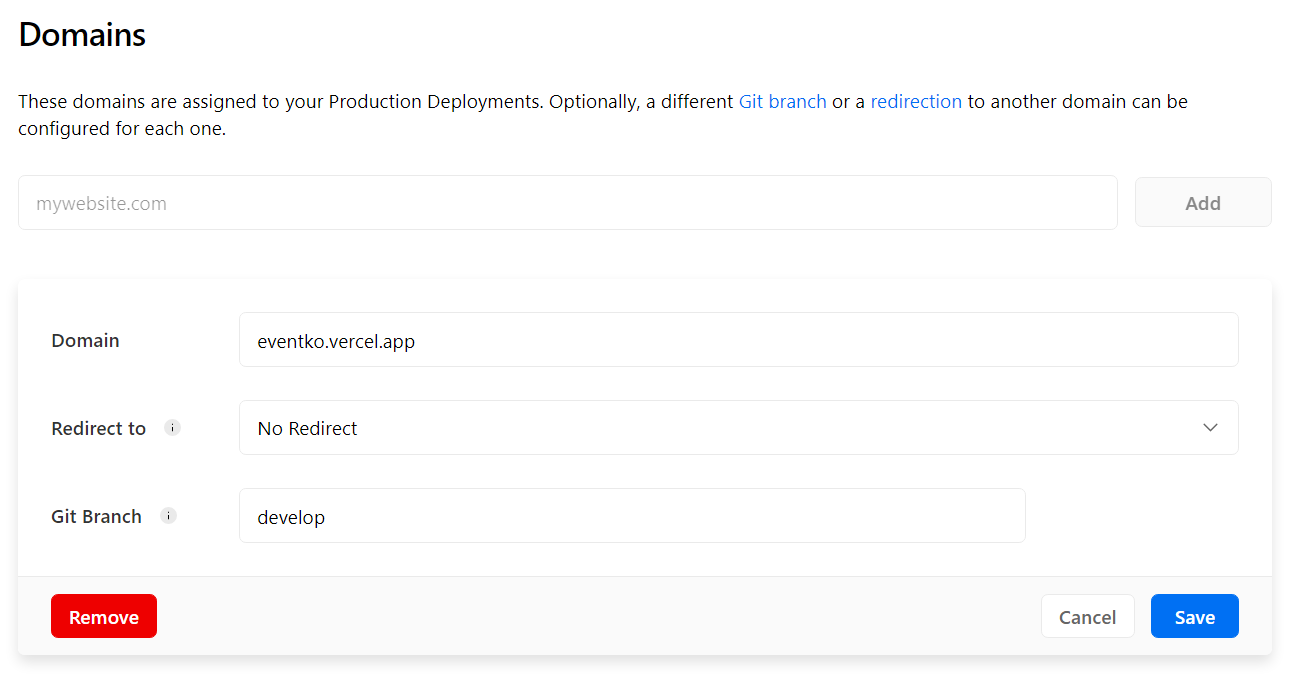
\includegraphics[width=\textwidth]{Opis deploymenta/Slika10.png}
					\caption{Promjena domene web-stranice}
				\end{figure}
			\end{packed_enum}
			
			\eject
	\chapter{Zaključak i budući rad}
		
		\indent U našoj smo skupini Vidoje odlučiti razviti u potpunosti novu ideju projektnog zadatka - interaktivni socijalni kalendar po uzoru na famozni Ferko prof. Marka Čupića, skrojen da pojednostavi praćenje obveza i uskladi akademski i društveni život prosječnom Ferovcu ili Ferovki. Rad na projektu sadržavao je mnoge neočekivane izazove i zapreke, no uz discipliniranu i marljivu suradnju sve su premoštene bez prevelikih muka.
		
		\indent Prvo i možda najbitnije bilo je osmisliti originalan zadatak kako bi se njegova složenost podudarala s onim zadanim. Ideju kalendara s događajima detaljno smo razradili, ubacili dodatne idejne funkcionalnosti i opcije kako bi konkurirao i predali na odobrenje nositelja predmeta. Neposredno nakon dobivanja potvrde nastavnika da je Eventko prošao provjeru, oformili smo podjedinice za frontend, backend i dokumentaciju te počeli s raspodjelom rada na incijalnim koracima projekta. Kao zajednički oslonac koristili smo rukom crtanu skicu koja prikazuje izgled početne stranice i njezino grananje na razne funkcionalnosti.
		
		\indent Tokom izrade Eventka skrenuli smo s nekih originalnih ideja poput korištenja QR kodova za dodavanje prijatelja i Google karte ukomponirane u odabir lokacije događaja, a dodali smo neke nove poput unosa kreditne kartice pri "plaćanju" za premium račun. Bilo je slučajeva u kojima se isti posao morao raditi više puta ispočetka zbog ranijeg brzanja ili neopreznosti, ali dobro planiranje svelo je ovakve instance na minimum.
		
		\indent Zajedničko stvaranje web-aplikacije u gotovo poslovnom okruženju koristilo je kao esencijalno iskustvo svakome od članova. Rijetko kada smo morali postavljati stroge vremenske rokove, no kada jesmo bili su poštovani i sav je posao obavljen na vrijeme. Eventko ima još prostora za potencijalna buduća unapređenja koja smo mogli ostvariti uz malo više vremena i vještine, poglavito stvaranje mobilne aplikacije da ga približi idejnim korisnicima. Zadovoljni smo vremenom uloženim u projekt, konačnim rezultatom te znanjem koje smo stekli radeći ga.
		
		\eject 
	\chapter*{Popis literature}
		\addcontentsline{toc}{chapter}{Popis literature}
	 	
 		\textbf{\textit{Kontinuirano osvježavanje}}
		
		
		\begin{enumerate}
			
			
			\item  Programsko inženjerstvo, FER ZEMRIS, \url{http://www.fer.hr/predmet/proinz}
			
			\item  I. Sommerville, "Software engineering", 8th ed, Addison Wesley, 2007.
			
			\item  T.C.Lethbridge, R.Langaniere, "Object-Oriented Software Engineering", 2nd ed. McGraw-Hill, 2005.
			
			\item  I. Marsic, Software engineering book``, Department of Electrical and Computer Engineering, Rutgers University, \url{http://www.ece.rutgers.edu/~marsic/books/SE}
			
			\item  The Unified Modeling Language, \url{https://www.uml-diagrams.org/}
			
			\item  Astah Community, \url{http://astah.net/editions/uml-new}
		\end{enumerate}
		
		 
	
	
	\begingroup
	\renewcommand*\listfigurename{Indeks slika i dijagrama}
	%\renewcommand*\listtablename{Indeks tablica}
	%\let\clearpage\relax
	\listoffigures
	%\vspace{10mm}
	%\listoftables
	\endgroup
	\addcontentsline{toc}{chapter}{Indeks slika i dijagrama}


	
	\eject 
		
	\chapter*{Dodatak: Prikaz aktivnosti grupe}
		\addcontentsline{toc}{chapter}{Dodatak: Prikaz aktivnosti grupe}
		
		\section*{Dnevnik sastajanja}
		
		\begin{packed_enum}
			\item  sastanak
			
			\item[] \begin{packed_item}
				\item Datum: u ovom formatu: 20. listopada 2022.
				\item Prisustvovali: svi članovi tima
				\item Teme sastanka:
				\begin{packed_item}
					\item  sastanak s asistentom i demonstratorom
					\item  raščišćavanje elemenata projektnog zadatka
					\item  predaja alternativnog "Eventko" projekta
				\end{packed_item}
			\end{packed_item}
			
			\item  sastanak
			\item[] \begin{packed_item}
				\item Datum: u ovom formatu: 24. listopada 2022.
				\item Prisustvovali: svi članovi tima
				\item Teme sastanka:
				\begin{packed_item}
					\item  razrada koncepta projekta
					\item  osmišljavanje dodatnih funkcionalnosti, aktera
					\item  prijedlog podjele uloga
				\end{packed_item}
			\end{packed_item}
		
			\item  sastanak
			\item[] \begin{packed_item}
				\item Datum: u ovom formatu: 27. listopada 2022.
				\item Prisustvovali: svi članovi tima
				\item Teme sastanka:
				\begin{packed_item}
					\item  finalna podjela uloga
					\item  odabir radnog okruženja
				\end{packed_item}
			\end{packed_item}
		
			\item  sastanak
			\item[] \begin{packed_item}
				\item Datum: u ovom formatu: 3. studenog 2022.
				\item Prisustvovali: svi članovi tima
				\item Teme sastanka:
				\begin{packed_item}
					\item  instalacija potrebne programske potpore
					\item  detaljna skica funkcionalnosti stranice
					\item  daljnja podjela rada
					\item  dizajn originalnog logotipa
				\end{packed_item}
			\end{packed_item}
		
			\item  sastanak
			\item[] \begin{packed_item}
				\item Datum: u ovom formatu: 14. studenog 2022.
				\item Prisustvovali: svi članovi tima
				\item Teme sastanka:
				\begin{packed_item}
					\item  priprema za demonstraciju osnovnih funkcionalnosti
					\item  povezivanje backenda i frontenda
					\item  usklađivanje ograničenja
				\end{packed_item}
			\end{packed_item}
			
			%
			
		\end{packed_enum}
		
		\eject
		\section*{Tablica aktivnosti}
		
			\textbf{\textit{Kontinuirano osvježavanje}}\\
			
			 \textit{Napomena: Doprinose u aktivnostima treba navesti u satima po članovima grupe po aktivnosti.}

			\begin{longtblr}[
					label=none,
				]{
					vlines,hlines,
					width = \textwidth,
					colspec={X[7, l]X[1, c]X[1, c]X[1, c]X[1, c]X[1, c]X[1, c]X[1, c]}, 
					vline{1} = {1}{text=\clap{}},
					hline{1} = {1}{text=\clap{}},
					rowhead = 1,
				} 
				\multicolumn{1}{c|}{} & \multicolumn{1}{c|}{\rotatebox{90}{\textbf{Velimir Kovačić }}} & \multicolumn{1}{c|}{\rotatebox{90}{\textbf{Jakov Krčadinac }}} &	\multicolumn{1}{c|}{\rotatebox{90}{\textbf{Ana Marić }}} & \multicolumn{1}{c|}{\rotatebox{90}{\textbf{Ema Nekić }}} &	\multicolumn{1}{c|}{\rotatebox{90}{\textbf{Filip Perković }}} & \multicolumn{1}{c|}{\rotatebox{90}{\textbf{Fran Saganić }}} &	\multicolumn{1}{c|}{\rotatebox{90}{\textbf{Luka Srića }}} \\  
				Upravljanje projektom 		&  &  &  &  &  &  & \\ 
				Opis projektnog zadatka 	&  &  &  &  &  &  & \\ 
				
				Funkcionalni zahtjevi       &  &  &  &  &  &  &  \\ 
				Opis pojedinih obrazaca 	&  &  &  &  &  &  &  \\ 
				Dijagram obrazaca 			&  &  &  &  &  &  &  \\ 
				Sekvencijski dijagrami 		&  &  &  &  &  &  &  \\ 
				Opis ostalih zahtjeva 		&  &  &  &  &  &  &  \\ 

				Arhitektura i dizajn sustava	 &  &  &  &  &  &  &  \\ 
				Baza podataka				&  &  &  &  &  &  &   \\ 
				Dijagram razreda 			&  &  &  &  &  &  &   \\ 
				Dijagram stanja				&  &  &  &  &  &  &  \\ 
				Dijagram aktivnosti 		&  &  &  &  &  &  &  \\ 
				Dijagram komponenti			&  &  &  &  &  &  &  \\ 
				Korištene tehnologije i alati 		&  &  &  &  &  &  &  \\ 
				Ispitivanje programskog rješenja 	&  &  &  &  &  &  &  \\ 
				Dijagram razmještaja			&  &  &  &  &  &  &  \\ 
				Upute za puštanje u pogon 		&  &  &  &  &  &  &  \\  
				Dnevnik sastajanja 			&  &  &  &  &  &  &  \\ 
				Zaključak i budući rad 		&  &  &  &  &  &  &  \\  
				Popis literature 			&  &  &  &  &  &  &  \\  
				&  &  &  &  &  &  &  \\ \hline 
				\textit{Dodatne stavke kako ste podijelili izradu aplikacije} 			&  &  &  &  &  &  &  \\ 
				\textit{npr. izrada početne stranice} 				&  &  &  &  &  &  &  \\  
				\textit{izrada baze podataka} 		 			&  &  &  &  &  &  & \\  
				\textit{spajanje s bazom podataka} 							&  &  &  &  &  &  &  \\ 
				\textit{back end} 							&  &  &  &  &  &  &  \\  
				 							&  &  &  &  &  &  &\\ 
			\end{longtblr}
					
					
		\eject
		\section*{Dijagrami pregleda promjena}
		
		\textbf{\textit{dio 2. revizije}}\\
		
		\textit{Prenijeti dijagram pregleda promjena nad datotekama projekta. Potrebno je na kraju projekta generirane grafove s gitlaba prenijeti u ovo poglavlje dokumentacije. Dijagrami za vlastiti projekt se mogu preuzeti s gitlab.com stranice, u izborniku Repository, pritiskom na stavku Contributors.}
		
	


\end{document} %naredbe i tekst nakon ove naredbe ne ulaze u izgrađen dokument 


